\chapter{Results}
\label{ch:results}

This chapter presents the results of applying PageRank and HITS to the football transfer network and interpreting the outcomes through the \textit{Transfer Analyzer} system. The purpose of the chapter is not merely to display rankings, but to explain what kinds of structural insights emerge when the same graph is analyzed through different algorithmic perspectives, weighting schemes, temporal filters, and visualization modes.

The results are organized around the experimental setting, the evaluation dimensions, and the major analytical views provided by the implemented web application. Since the application supports interactive exploration, the chapter also discusses how different visual modes contribute to the interpretation of ranking behavior.


%=============================================================
\section{Experimental Setting and Dataset}
\label{sec:results_setting}

The experiments were conducted on the football transfer dataset described in Chapter~\ref{ch:background}. The dataset contains player transfer records spanning multiple seasons and leagues, with each row representing one transfer event between a selling club and a buying club. After preprocessing and aggregation, the dataset is transformed into a weighted directed graph where clubs are nodes and transfer relations are edges.

The implemented analytical system supports both full-network analysis and filtered analysis. Accordingly, the experiments in this thesis were carried out under the following settings:
\begin{itemize}
    \item \textbf{Algorithm selection:} PageRank and HITS;
    \item \textbf{Direction of analysis:} buyer-oriented and seller-oriented;
    \item \textbf{Weighting mode:} transfer fee and transfer count;
    \item \textbf{League scope:} all available leagues or a selected intra-league subset;
    \item \textbf{Temporal scope:} all seasons or an inclusive season range;
    \item \textbf{Visualization scope:} top-$N$ ranked clubs, with $N$ configurable by the user.
\end{itemize}

The default configuration of the application emphasizes a top-ranked subset of clubs rather than the entire graph. This improves interpretability, especially in the interactive network and chart views, while still preserving the most analytically relevant outcomes of each algorithm.


%=============================================================
\section{Tools Used}
\label{sec:results_tools}

The experiments and outputs described in this chapter were produced using the \textit{Transfer Analyzer} system implemented in this thesis. The main tools used are:
\begin{itemize}
    \item \textbf{PySpark and Apache Spark} for data loading, graph construction, and iterative score computation;
    \item \textbf{FastAPI} for exposing the ranking computations and dataset queries as backend services;
    \item \textbf{Chart.js} for ranked bar-chart visualizations;
    \item \textbf{Cytoscape.js} for interactive network graph visualizations;
    \item \textbf{D3.js} for the animated historical ranking view and flow-based visual exploration.
\end{itemize}

The combined use of these tools allows the thesis to move beyond static ranking tables and instead support an interactive style of experimental interpretation.


%=============================================================
\section{Evaluation Dimensions}
\label{sec:results_eval_dimensions}

The comparative interpretation of results in this thesis is based on several complementary dimensions:
\begin{enumerate}
    \item the clubs ranked highest by each algorithm;
    \item the differences between buyer-oriented and seller-oriented analysis;
    \item the differences between fee-weighted and count-weighted graphs;
    \item the effect of applying league and season filters;
    \item the degree of overlap between PageRank and HITS rankings;
    \item the visual patterns revealed through network, flow, and historical views.
\end{enumerate}

These dimensions make it possible to compare not only the numerical outputs of PageRank and HITS, but also the different structural stories they tell about the football transfer market.


%=============================================================
\section{PageRank and HITS Ranking Behavior}
\label{sec:results_ranking_behavior}

\subsection{Buyer-Oriented Analysis}
\label{subsec:results_buyers}

When the graph is analyzed from the buyer perspective, both algorithms identify clubs that act as major attractors in the transfer market. In PageRank, a buyer club receives a high score when it attracts transfers from clubs that are themselves structurally significant in the network. This produces a notion of global importance: a club is important not simply because it buys many players, but because it buys from influential sellers.

HITS authority scores provide a related but distinct interpretation. A club becomes a strong authority when it receives transfers from strong hubs, that is, from clubs that are themselves strongly connected as suppliers. In practice, this means that authority rankings often emphasize structurally recognized destination clubs, but they may order them differently than PageRank because HITS separates the notions of receiving importance and distributing importance.

From an analytical standpoint, this distinction is significant. PageRank answers the question of which buyer clubs are globally central in the transfer ecosystem, whereas HITS authority analysis answers the question of which clubs serve as recognized destinations within a hub--authority structure.

% Top 10 Buyers PageRank - Fee Weighted
\begin{figure}[H]
    \centering
    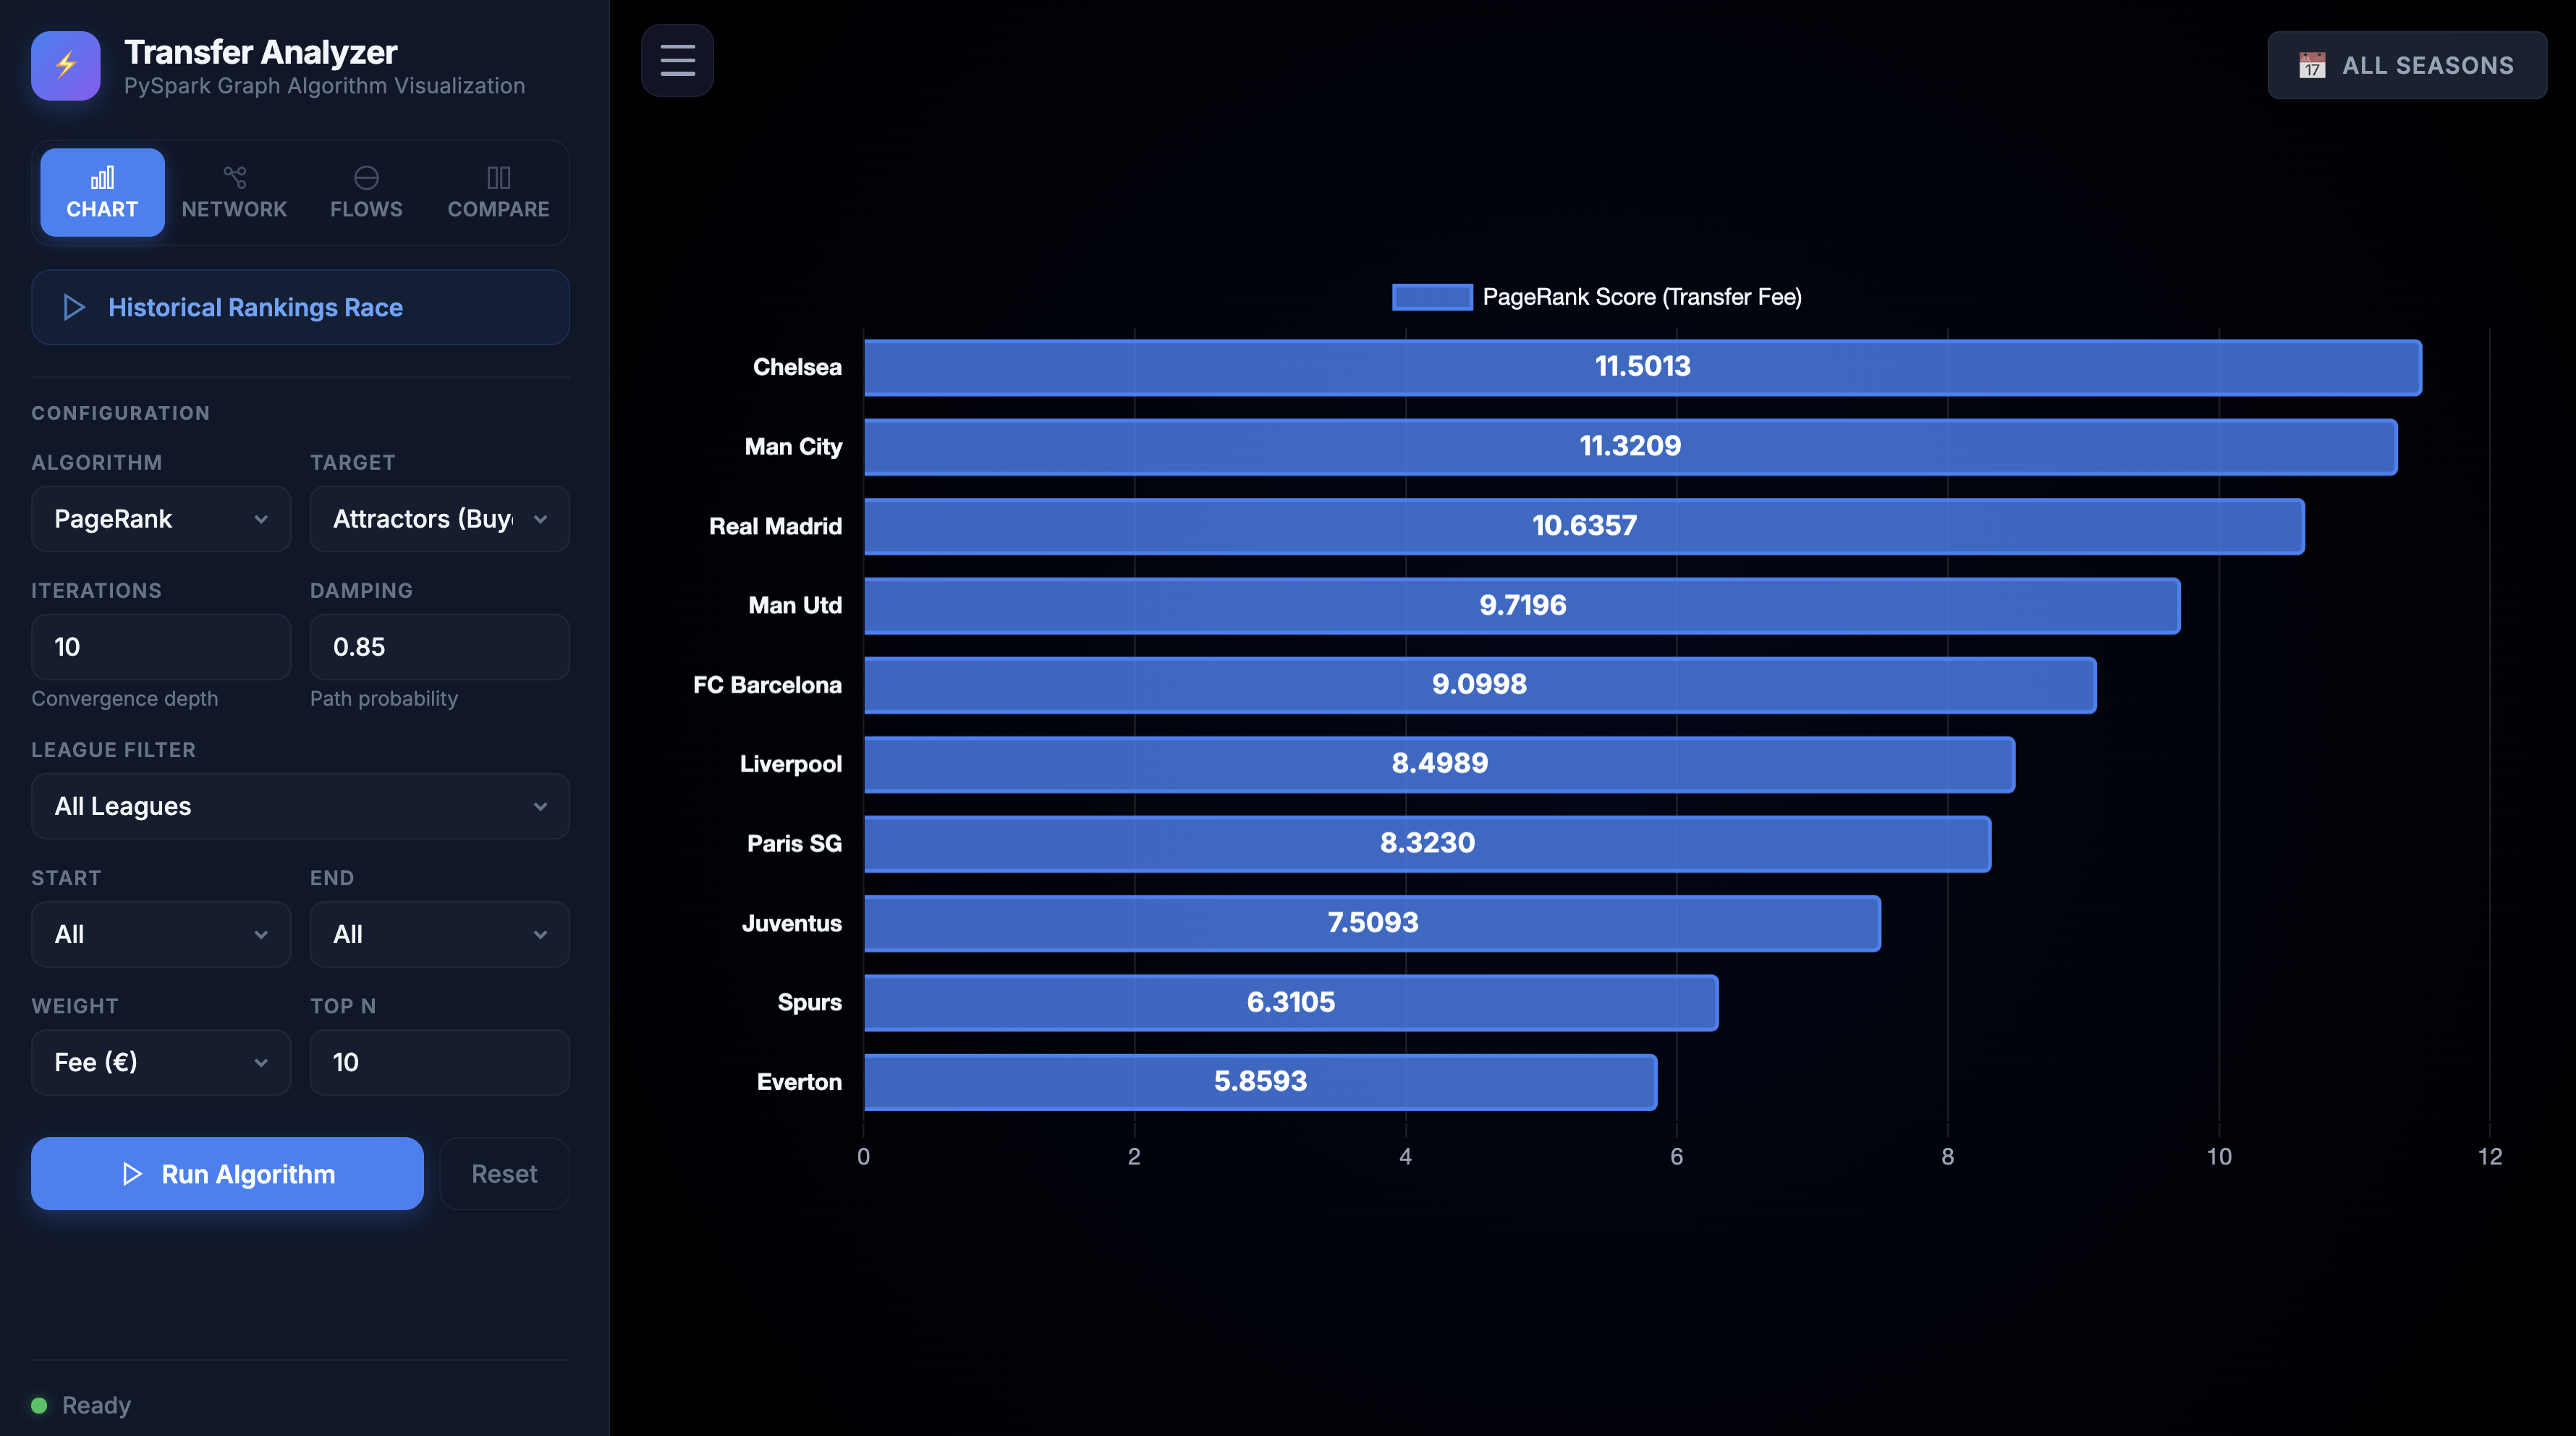
\includegraphics[width=1.0\textwidth]{Figures/ui_buyers_pagerank_fee.png}
    \caption{Application view for Top 10 Buyers PageRank (Fee Weighted)}
    \label{fig:ui_buyers_pagerank_fee}

    \vspace{1.5em}
    
    \begin{tabular}{|l|l|r|}
\hline
\textbf{Rank} & \textbf{Club} & \textbf{Score} \\
\hline
1 & Chelsea & 11.5013 \\
2 & Man City & 11.3209 \\
3 & Real Madrid & 10.6357 \\
4 & Man Utd & 9.7196 \\
5 & FC Barcelona & 9.0998 \\
6 & Liverpool & 8.4989 \\
7 & Paris SG & 8.3230 \\
8 & Juventus & 7.5093 \\
9 & Spurs & 6.3105 \\
10 & Everton & 5.8593 \\
\hline
\end{tabular}
    \captionof{table}{Top 10 Buyers PageRank - Fee Weighted}
    \label{tab:top_10_buyers_pagerank___fee_weighted}
\end{figure}

% Top 10 Authority Buyers HITS - Fee Weighted
\begin{figure}[H]
    \centering
    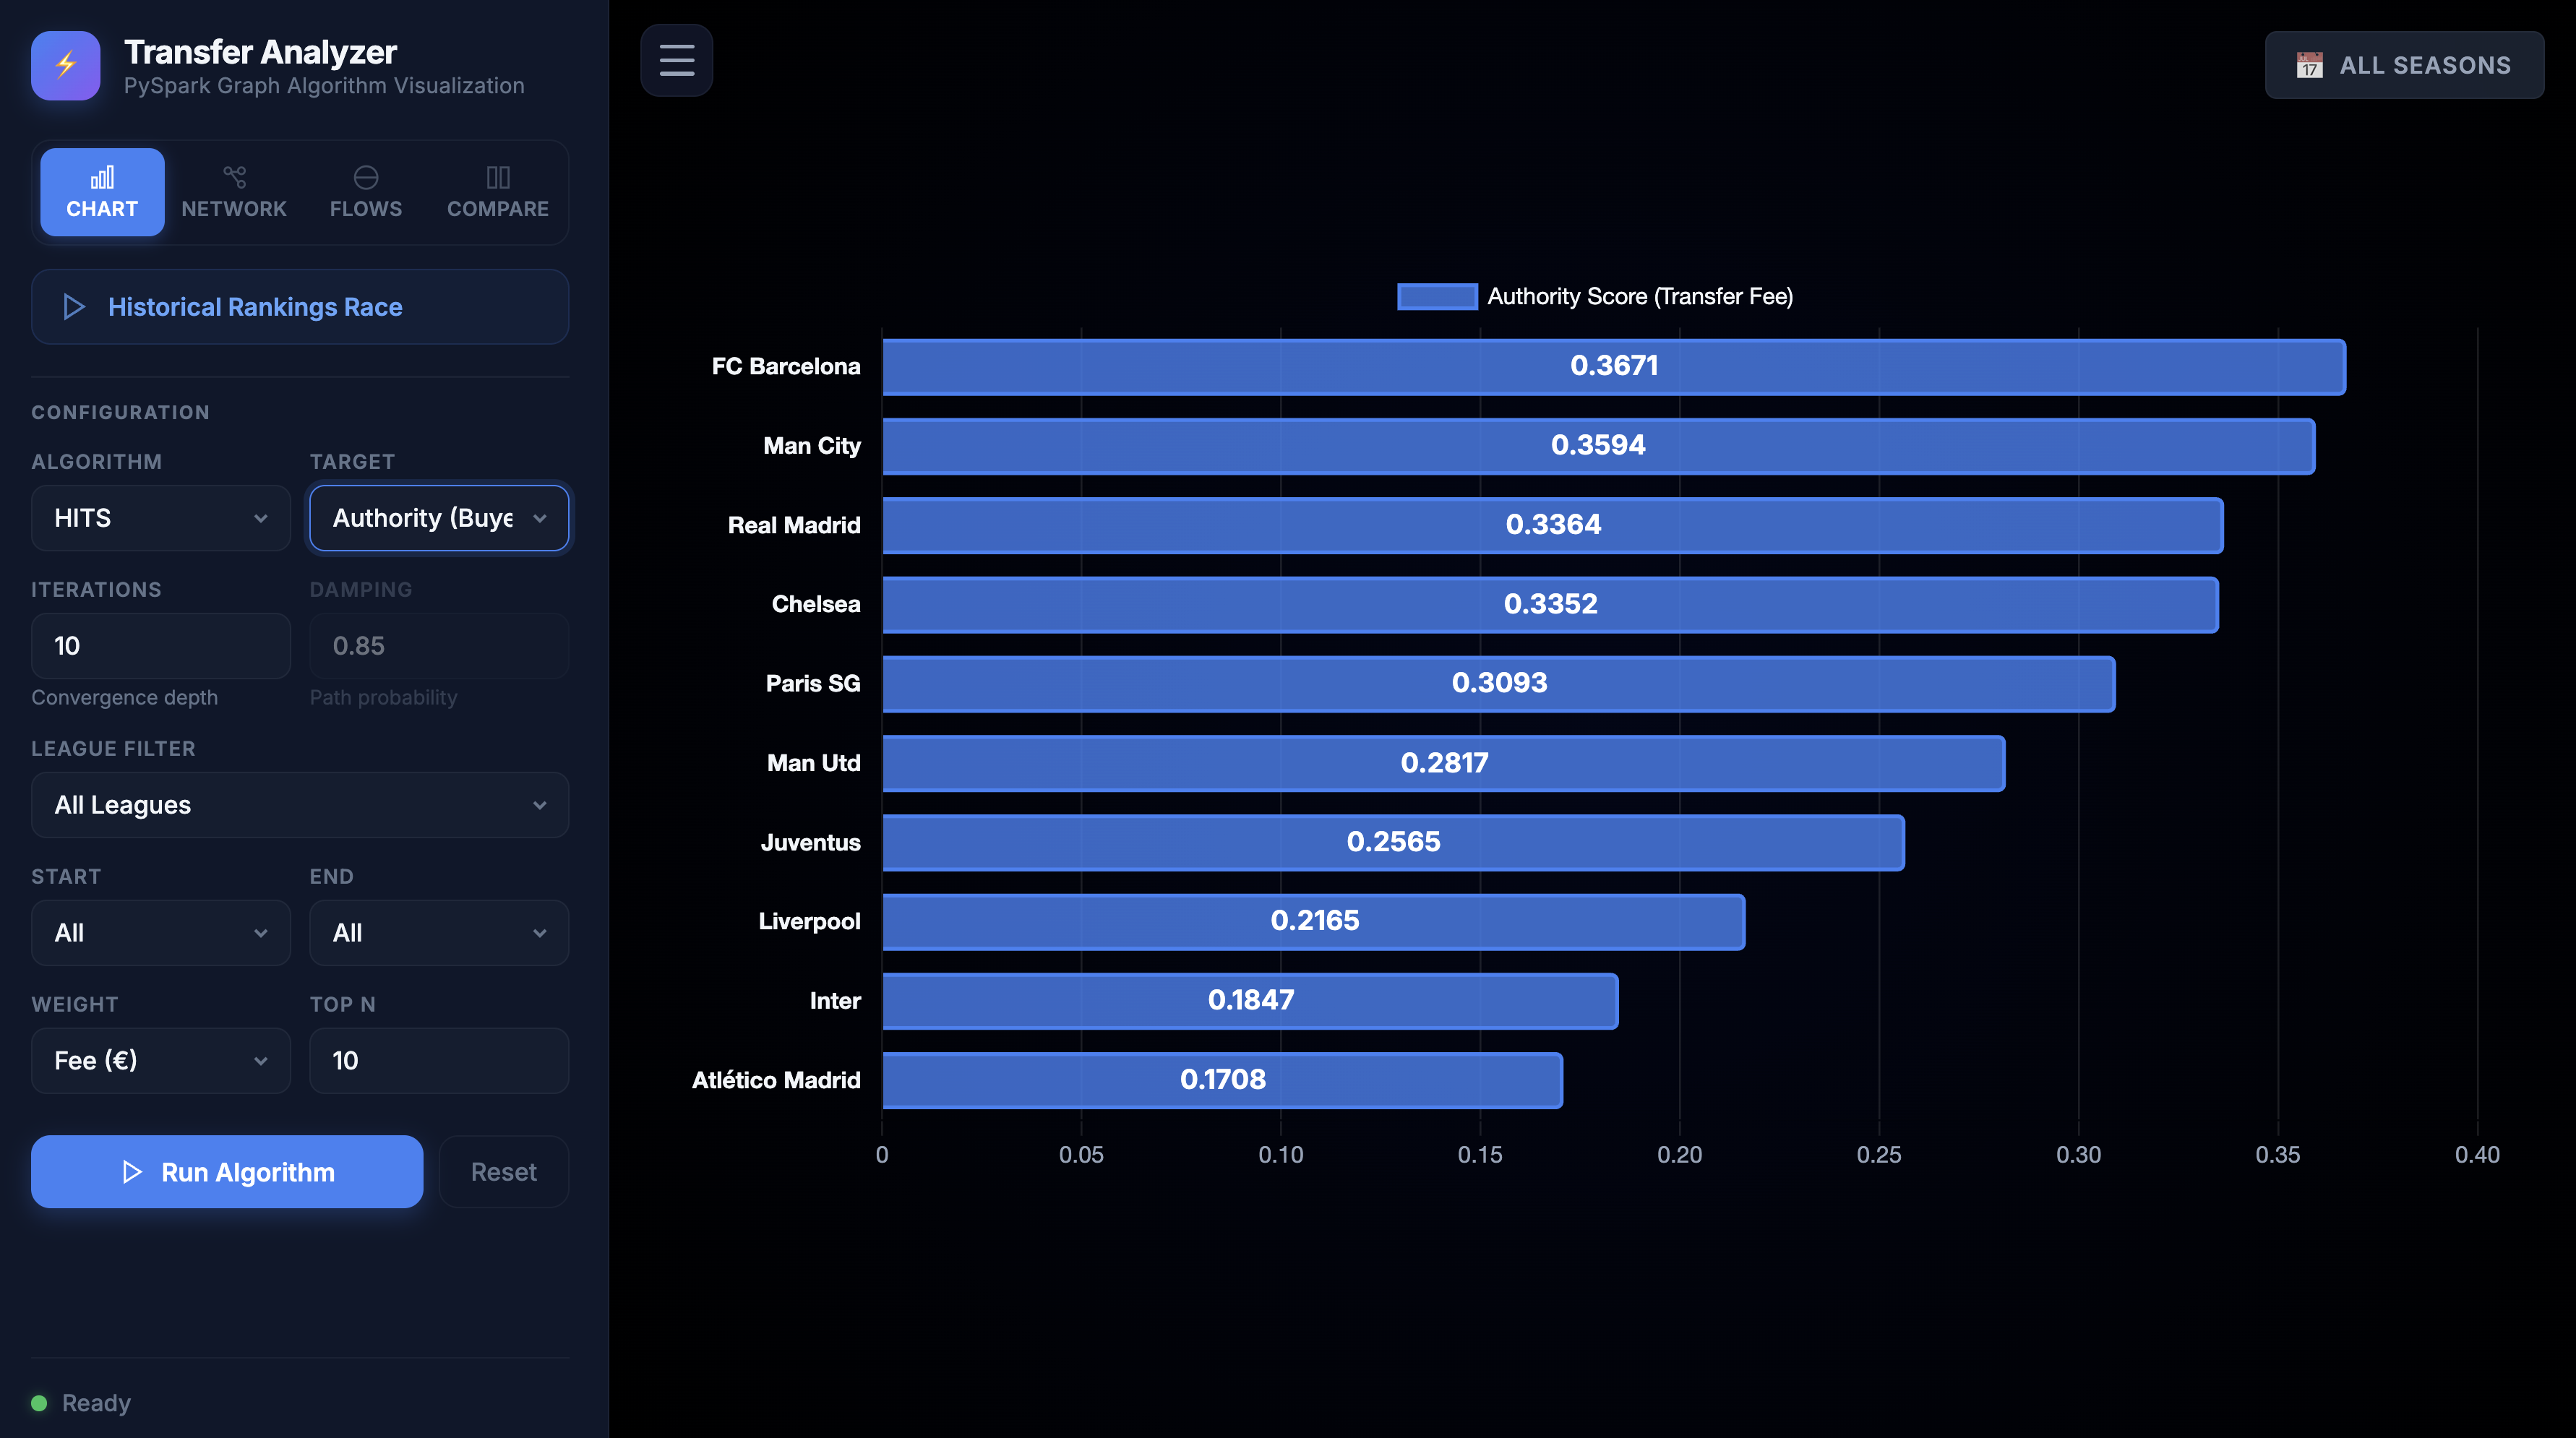
\includegraphics[width=1.0\textwidth]{Figures/ui_authority_buyers_hits_fee.png}
    \caption{Application view for Top 10 Authority Buyers HITS (Fee Weighted)}
    \label{fig:ui_authority_buyers_hits_fee}

    \vspace{1.5em}
    
    \begin{tabular}{|l|l|r|}
\hline
\textbf{Rank} & \textbf{Club} & \textbf{Score} \\
\hline
1 & FC Barcelona & 0.3671 \\
2 & Man City & 0.3594 \\
3 & Real Madrid & 0.3364 \\
4 & Chelsea & 0.3352 \\
5 & Paris SG & 0.3093 \\
6 & Man Utd & 0.2817 \\
7 & Juventus & 0.2565 \\
8 & Liverpool & 0.2165 \\
9 & Inter & 0.1847 \\
10 & Atlético Madrid & 0.1708 \\
\hline
\end{tabular}
    \captionof{table}{Top 10 Authority Buyers HITS - Fee Weighted}
    \label{tab:top_10_authority_buyers_hits___fee_weighted}
\end{figure}

\subsection{Seller-Oriented Analysis}
\label{subsec:results_sellers}

Seller-oriented analysis reveals another important difference between the two algorithms. In the implemented system, PageRank seller rankings are computed by reversing the edge direction so that clubs transferring players to important buyers receive higher supplier-oriented scores. This view highlights clubs that act as influential sources in the market.

HITS hub rankings naturally provide a structurally similar seller perspective without requiring a separate semantic reinterpretation of the algorithm. A club becomes a strong hub when it transfers players to strong authorities. This makes HITS particularly suitable for identifying supplier clubs that occupy an important intermediary or feeder role in the network.

The comparison between seller-oriented PageRank and hub-oriented HITS is therefore one of the most meaningful aspects of the thesis. It demonstrates that even when the two methods are aimed at a similar conceptual role, they reach that role through different mathematical mechanisms.

% Top 10 Sellers PageRank - Fee Weighted
\begin{figure}[H]
    \centering
    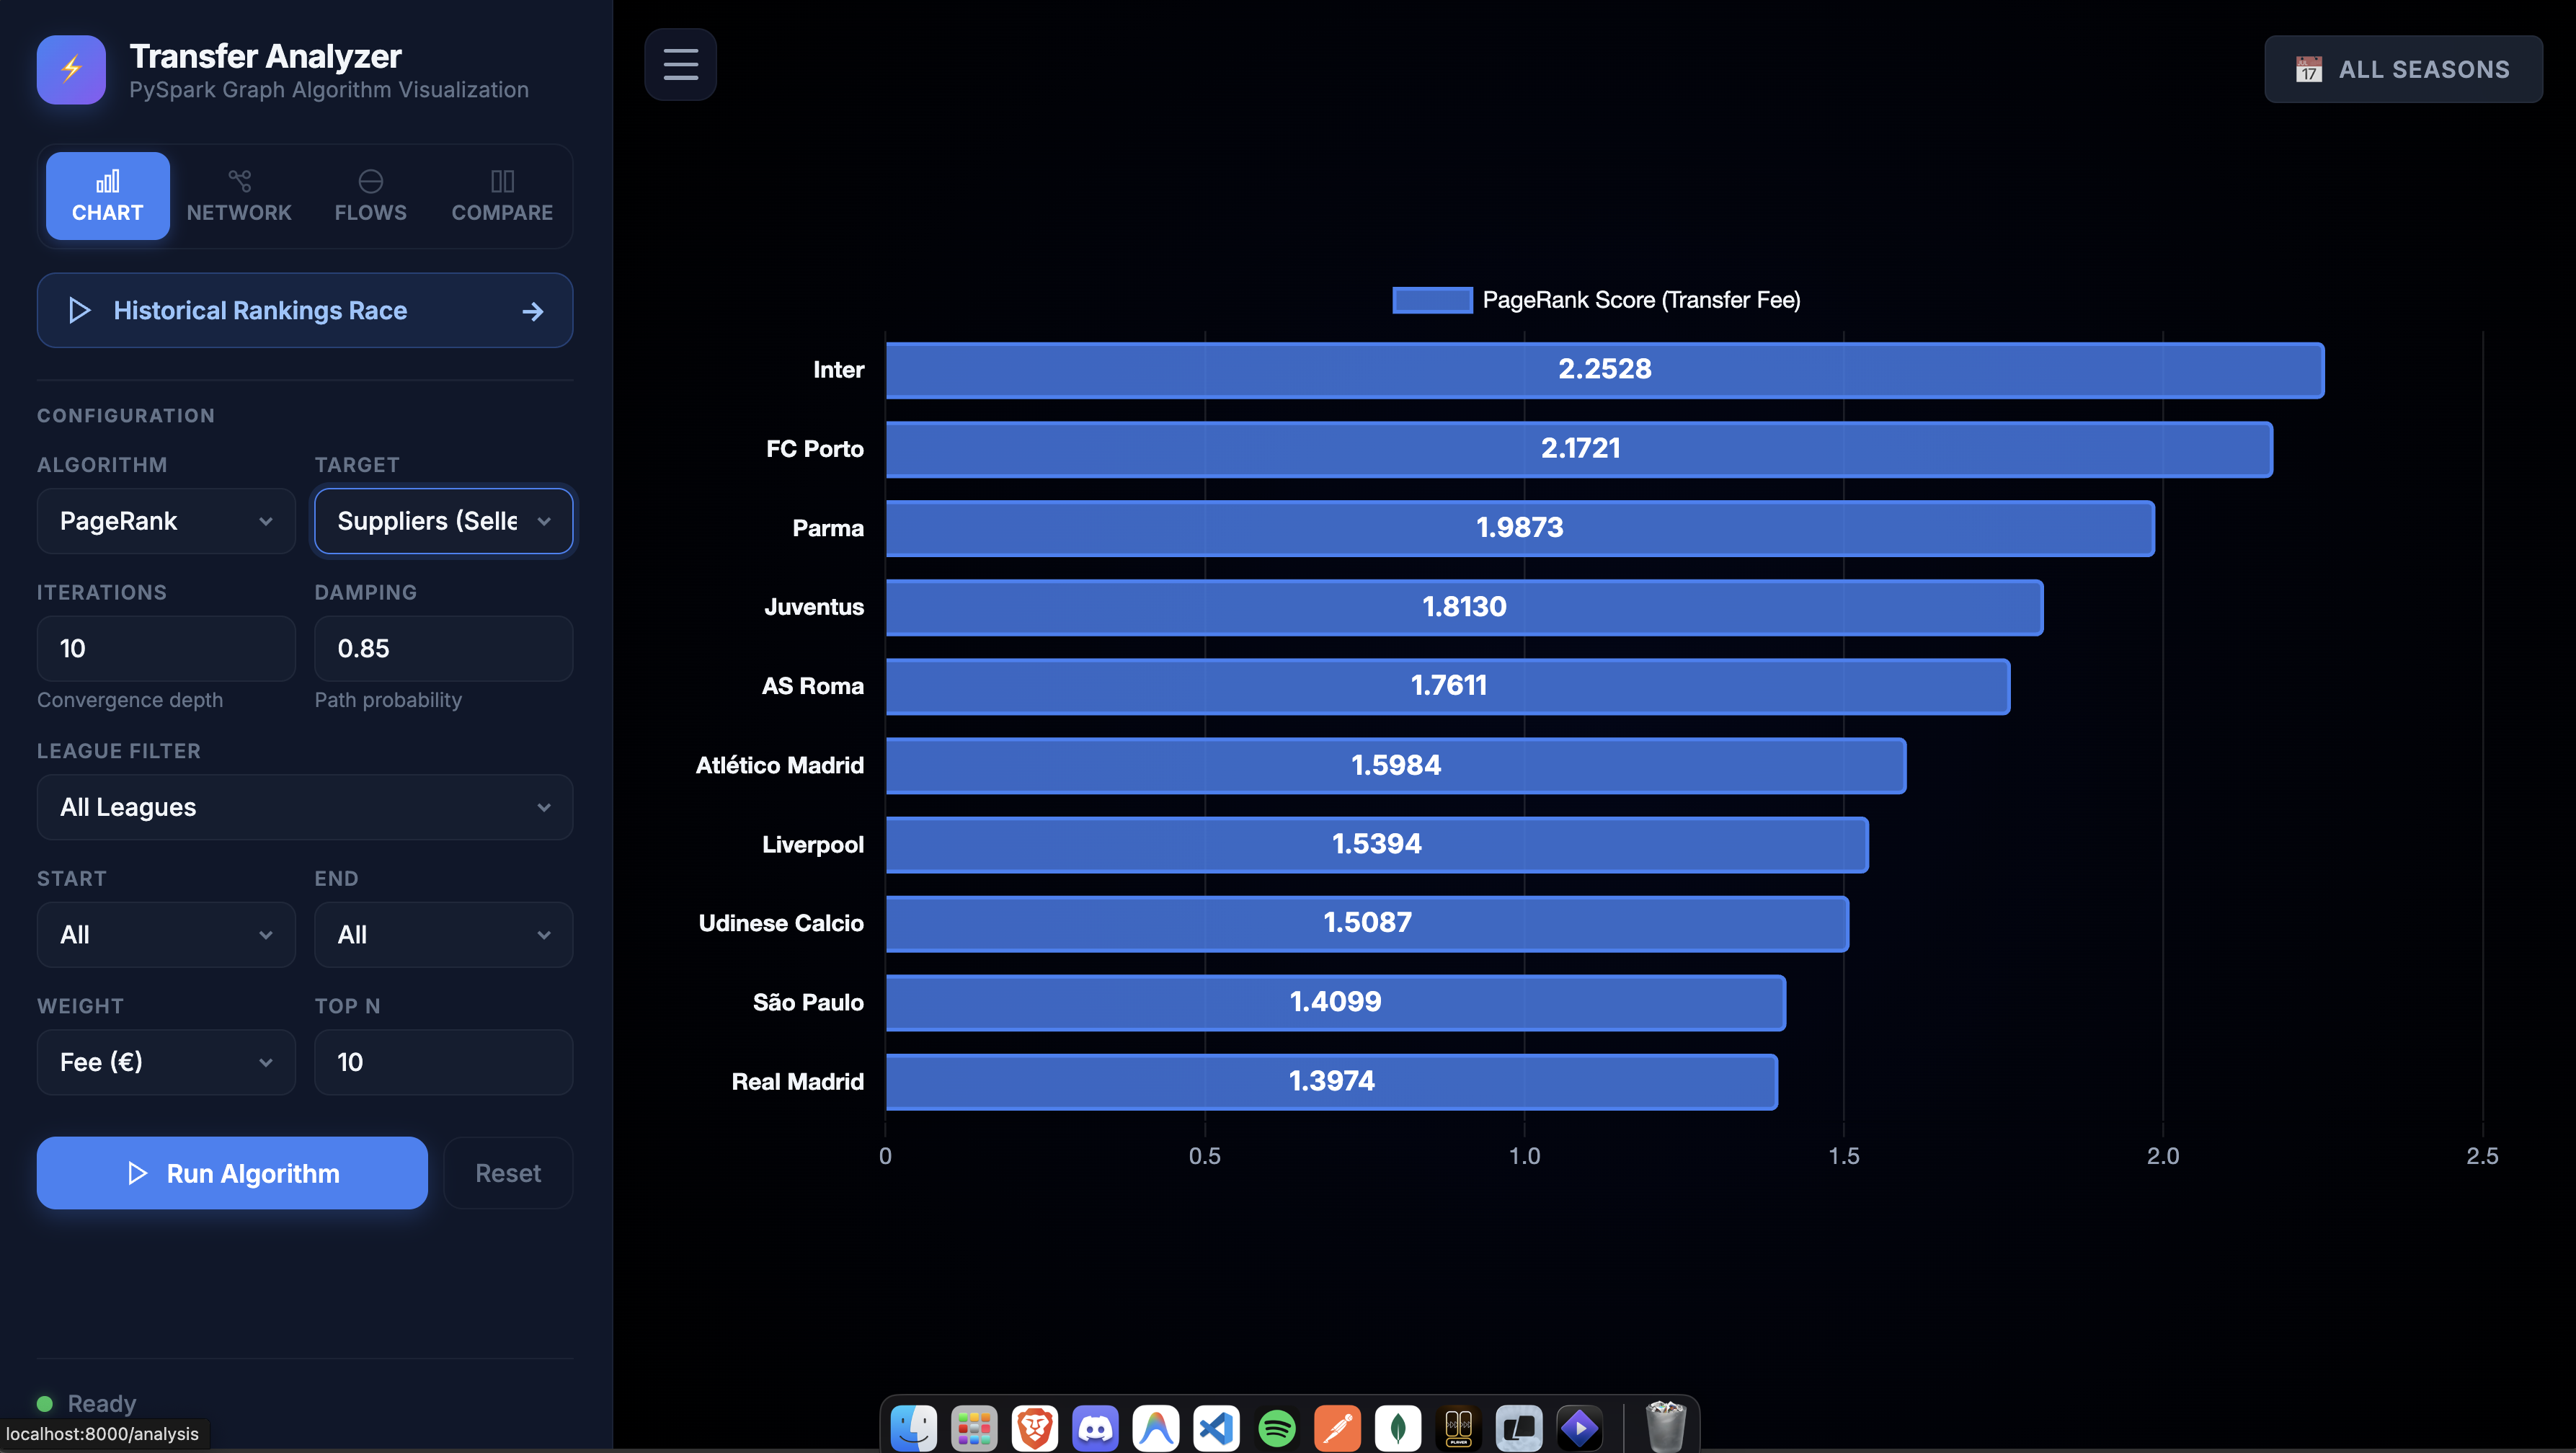
\includegraphics[width=1.0\textwidth]{Figures/ui_sellers_pagerank_fee.png}
    \caption{Application view for Top 10 Sellers PageRank (Fee Weighted)}
    \label{fig:ui_sellers_pagerank_fee}

    \vspace{1.5em}
    
    \begin{tabular}{|l|l|r|}
\hline
\textbf{Rank} & \textbf{Club} & \textbf{Score} \\
\hline
1 & Inter & 2.2528 \\
2 & FC Porto & 2.1721 \\
3 & Parma & 1.9873 \\
4 & Juventus & 1.8130 \\
5 & AS Roma & 1.7611 \\
6 & Atlético Madrid & 1.5984 \\
7 & Liverpool & 1.5394 \\
8 & Udinese Calcio & 1.5087 \\
9 & São Paulo & 1.4099 \\
10 & Real Madrid & 1.3974 \\
\hline
\end{tabular}
    \captionof{table}{Top 10 Sellers PageRank - Fee Weighted}
    \label{tab:top_10_sellers_pagerank___fee_weighted}
\end{figure}

% Top 10 Hubs Sellers HITS - Fee Weighted
\begin{figure}[H]
    \centering
    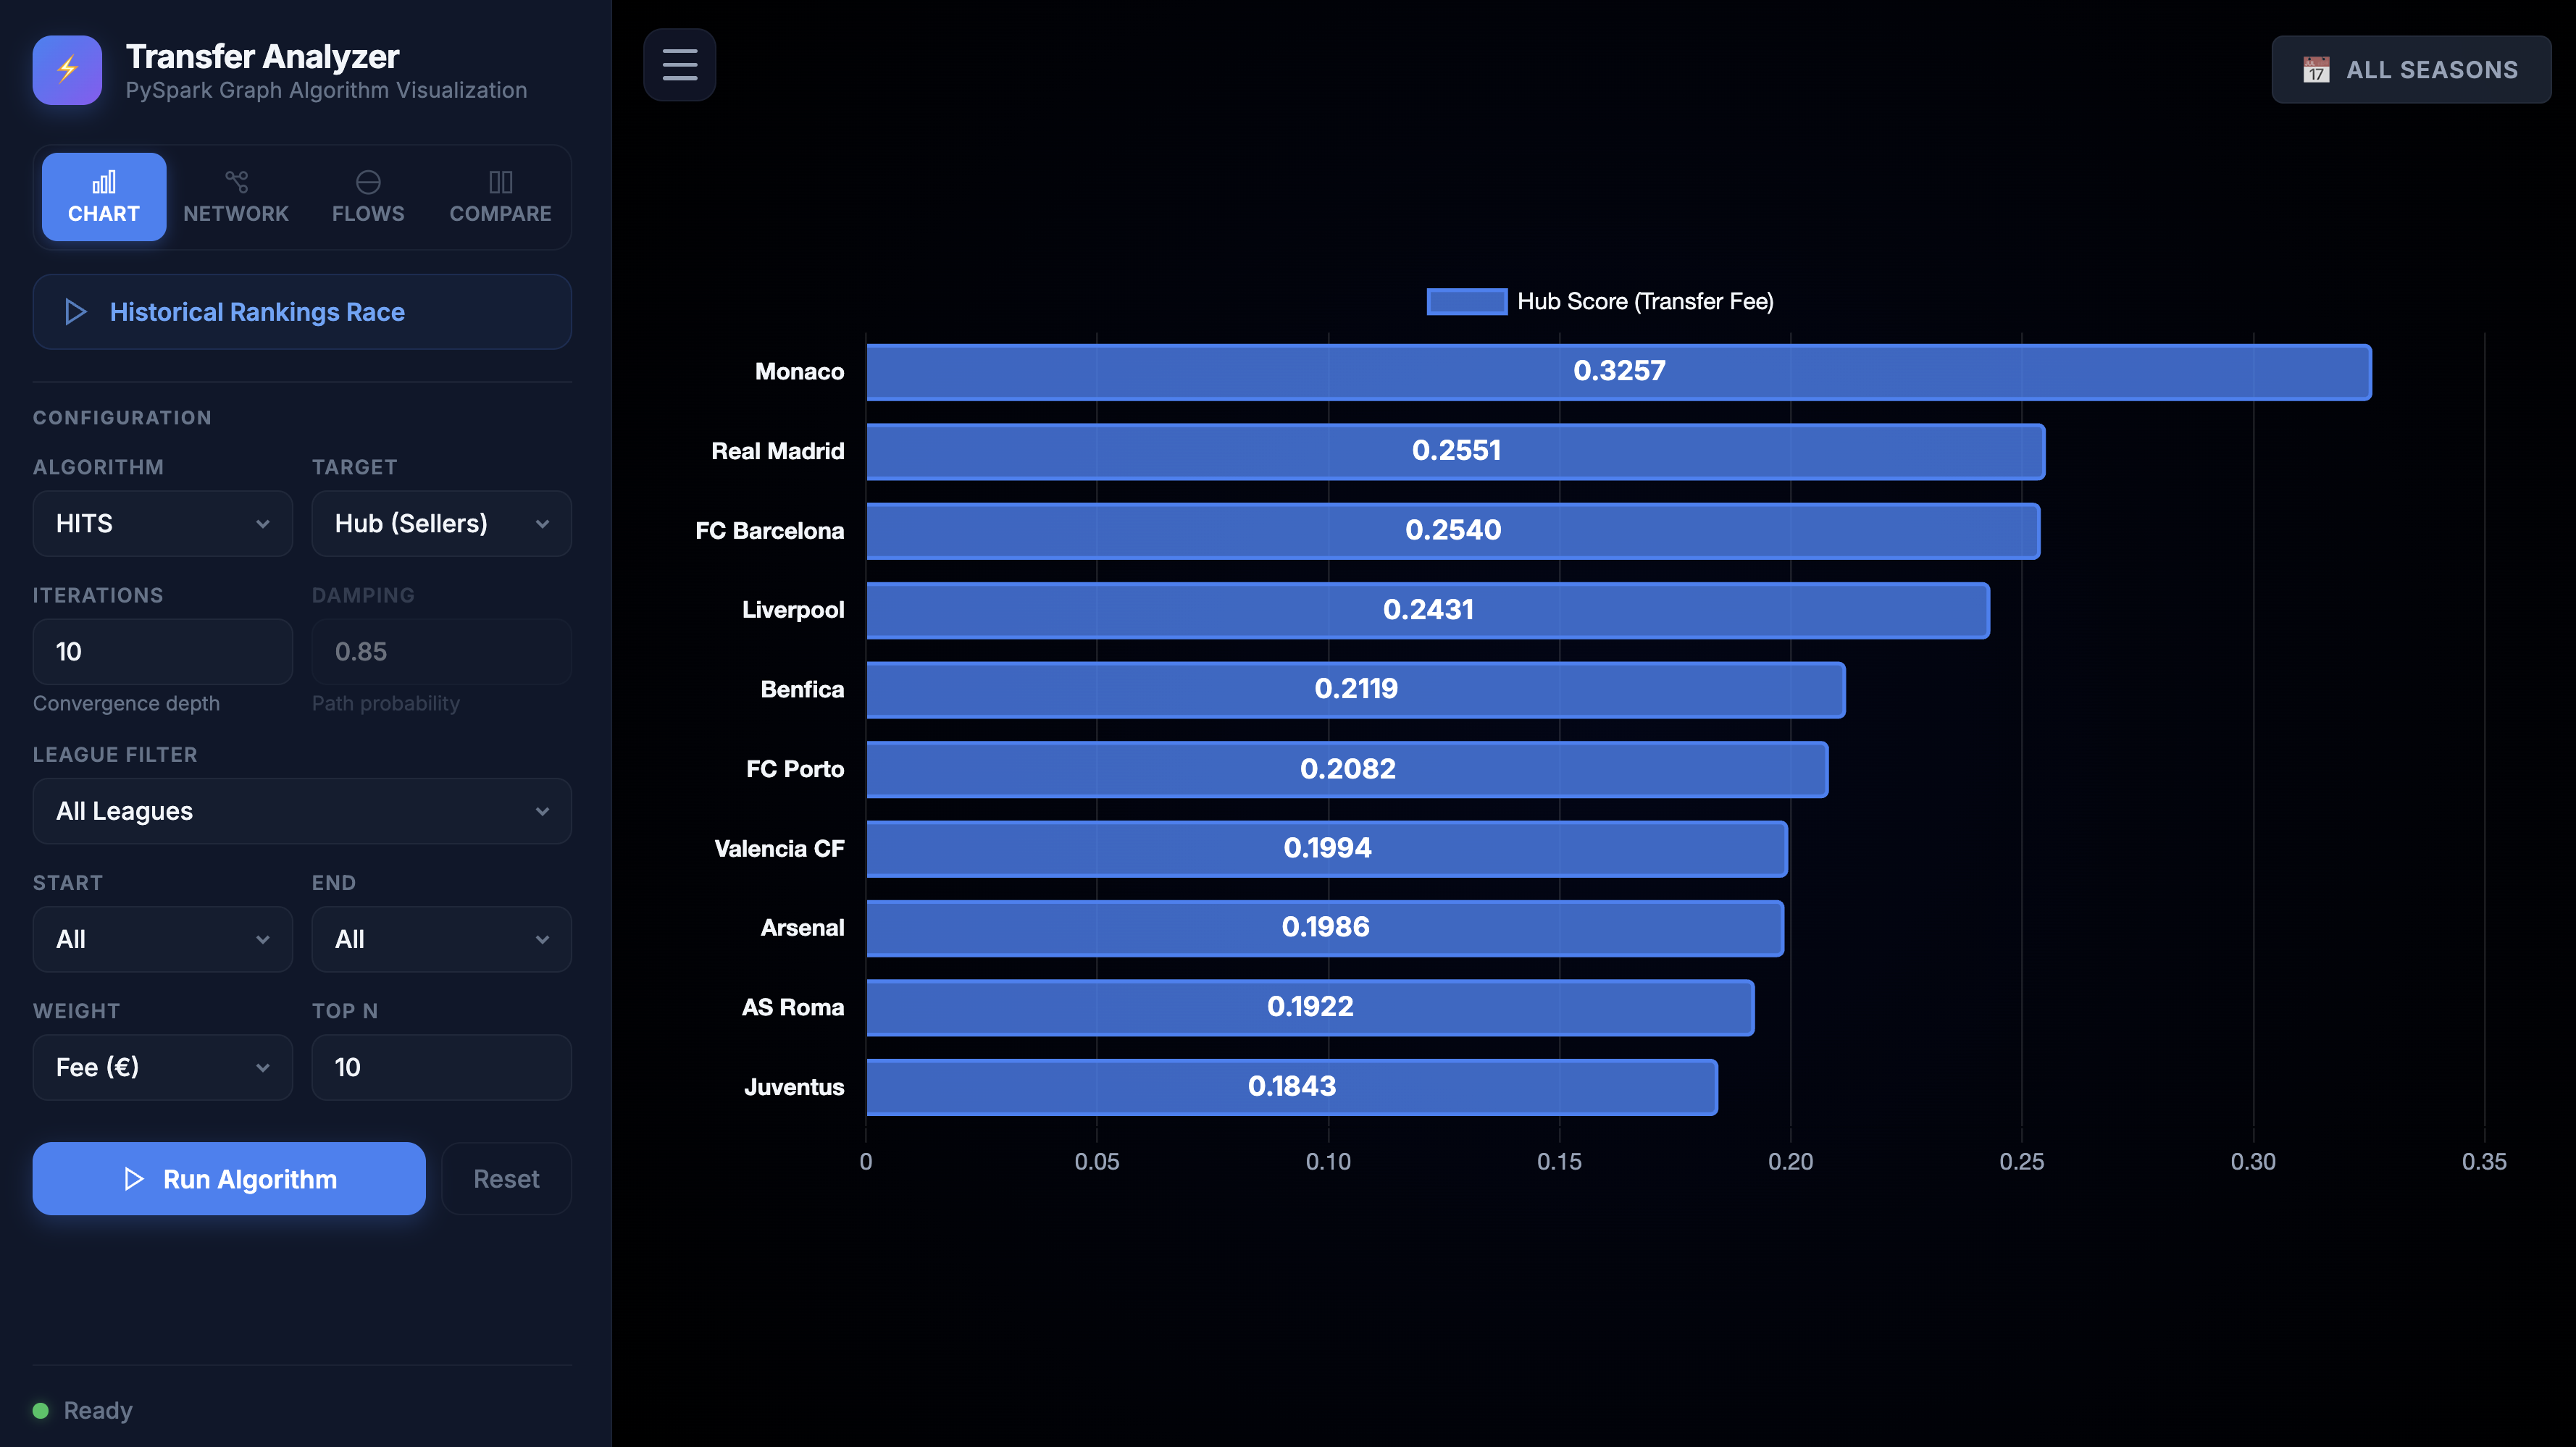
\includegraphics[width=1.0\textwidth]{Figures/ui_hubs_sellers_hits_fee.png}
    \caption{Application view for Top 10 Hubs Sellers HITS (Fee Weighted)}
    \label{fig:ui_hubs_sellers_hits_fee}

    \vspace{1.5em}
    
    \begin{tabular}{|l|l|r|}
\hline
\textbf{Rank} & \textbf{Club} & \textbf{Score} \\
\hline
1 & Monaco & 0.3257 \\
2 & Real Madrid & 0.2551 \\
3 & FC Barcelona & 0.2540 \\
4 & Liverpool & 0.2431 \\
5 & Benfica & 0.2119 \\
6 & FC Porto & 0.2082 \\
7 & Valencia CF & 0.1994 \\
8 & Arsenal & 0.1986 \\
9 & AS Roma & 0.1922 \\
10 & Juventus & 0.1843 \\
\hline
\end{tabular}
    \captionof{table}{Top 10 Hubs Sellers HITS - Fee Weighted}
    \label{tab:top_10_hubs_sellers_hits___fee_weighted}
\end{figure}

%=============================================================
\section{Effect of Weighting Mode}
\label{sec:results_weight_mode}

One of the most informative comparisons in the thesis concerns the choice of edge weighting. The same club may appear highly influential in one weighting mode and less influential in the other.

\subsection{Fee-Weighted Analysis}
\label{subsec:results_fee}

In fee-weighted mode, edges represent the total monetary value transferred between clubs. This favors clubs involved in financially large transfers and therefore tends to emphasize market power, financial reach, and participation in high-value player exchanges.

Under this mode, clubs associated with elite transfer markets are expected to dominate the top ranks, since the algorithmic importance flowing through the graph is proportional to the magnitude of transfer fees. As a result, fee-weighted analysis is especially useful for studying economic centrality and transfer-market prestige.

\subsection{Count-Weighted Analysis}
\label{subsec:results_count}

In count-weighted mode, every transfer contributes equally regardless of financial size. This shifts the interpretation from economic magnitude to transactional activity. Clubs with many repeated exchanges may rise in importance even if the average value of those exchanges is relatively modest.

This distinction is valuable because it prevents the study from reducing transfer importance to money alone. Count-based analysis captures activity intensity, while fee-based analysis captures financial weight. Comparing the two reveals whether a club's prominence comes from expensive transfers, frequent transfers, or a mixture of both.

% Top 10 Buyers PageRank - Count Weighted
\begin{figure}[H]
    \centering
    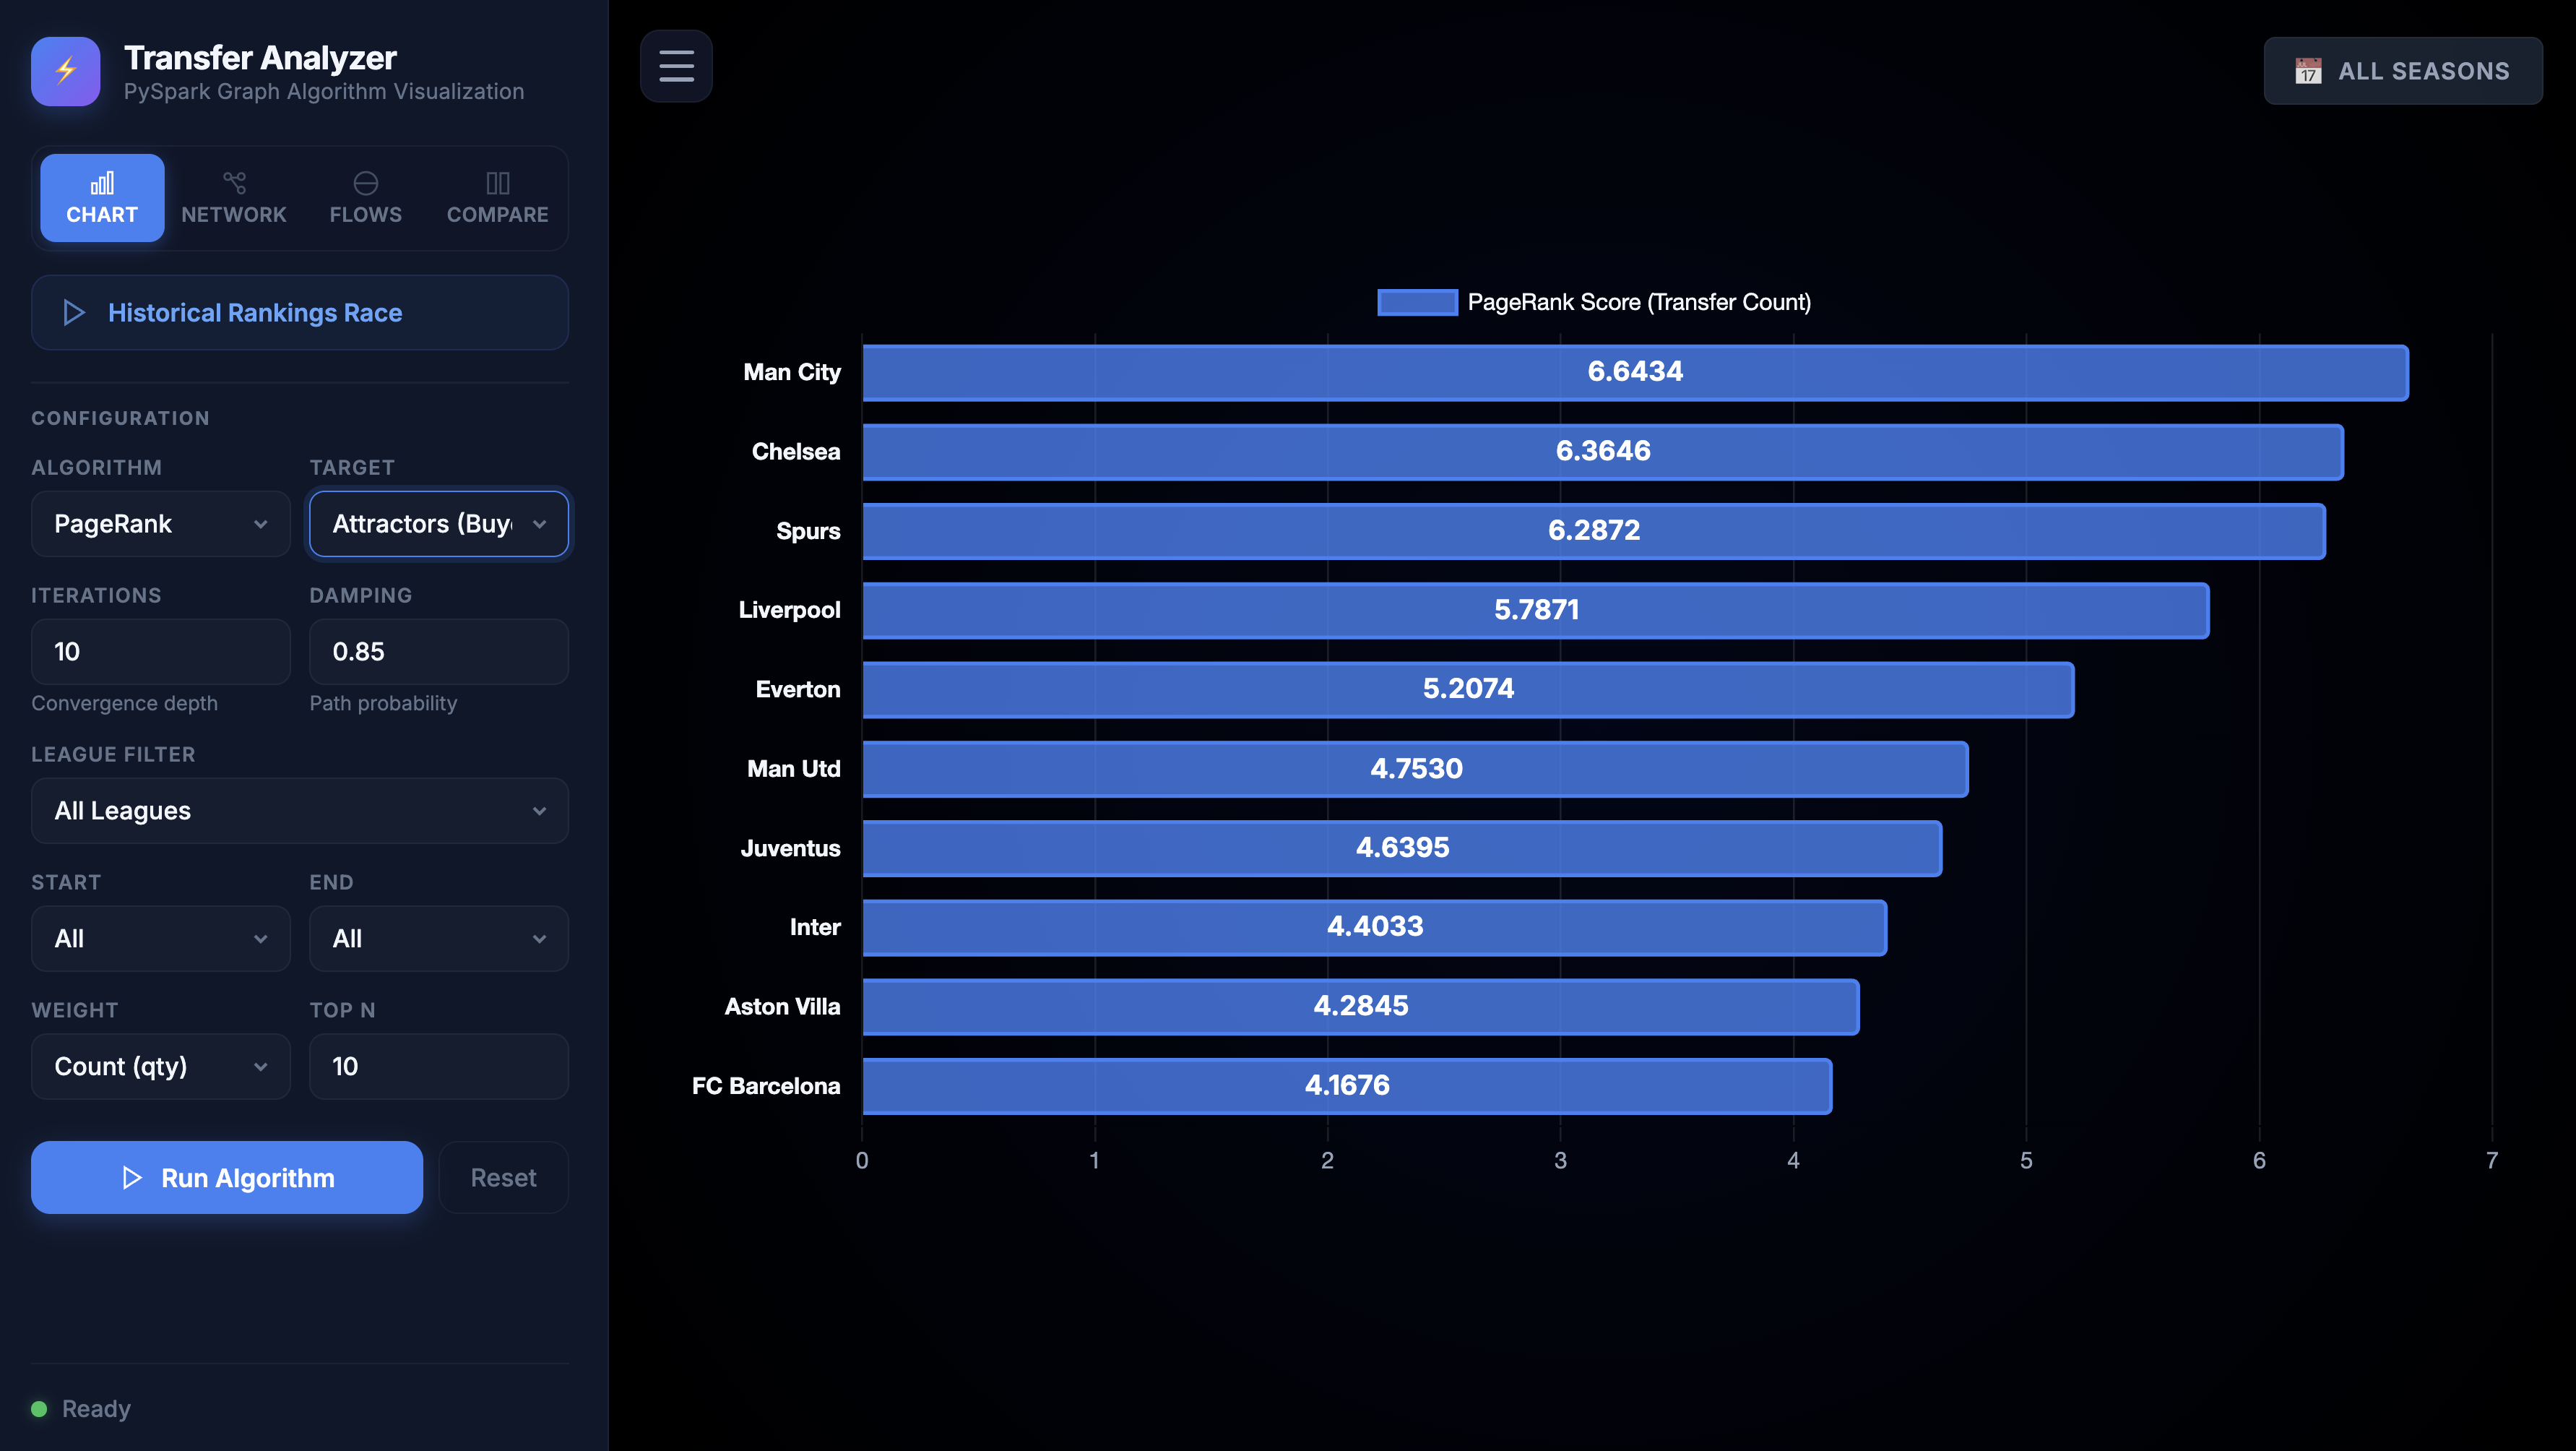
\includegraphics[width=1.0\textwidth]{Figures/ui_buyers_pagerank_count.png}
    \caption{Application view for Top 10 Buyers PageRank (Count Weighted)}
    \label{fig:ui_buyers_pagerank_count}

    \vspace{1.5em}
    
    \begin{tabular}{|l|l|r|}
\hline
\textbf{Rank} & \textbf{Club} & \textbf{Score} \\
\hline
1 & Man City & 6.6434 \\
2 & Chelsea & 6.3646 \\
3 & Spurs & 6.2872 \\
4 & Liverpool & 5.7871 \\
5 & Everton & 5.2074 \\
6 & Man Utd & 4.7530 \\
7 & Juventus & 4.6395 \\
8 & Inter & 4.4033 \\
9 & Aston Villa & 4.2845 \\
10 & FC Barcelona & 4.1676 \\
\hline
\end{tabular}
    \captionof{table}{Top 10 Buyers PageRank - Count Weighted}
    \label{tab:top_10_buyers_pagerank___count_weighted}
\end{figure}

% Top 10 Authority Buyers HITS - Count Weighted
\begin{figure}[H]
    \centering
    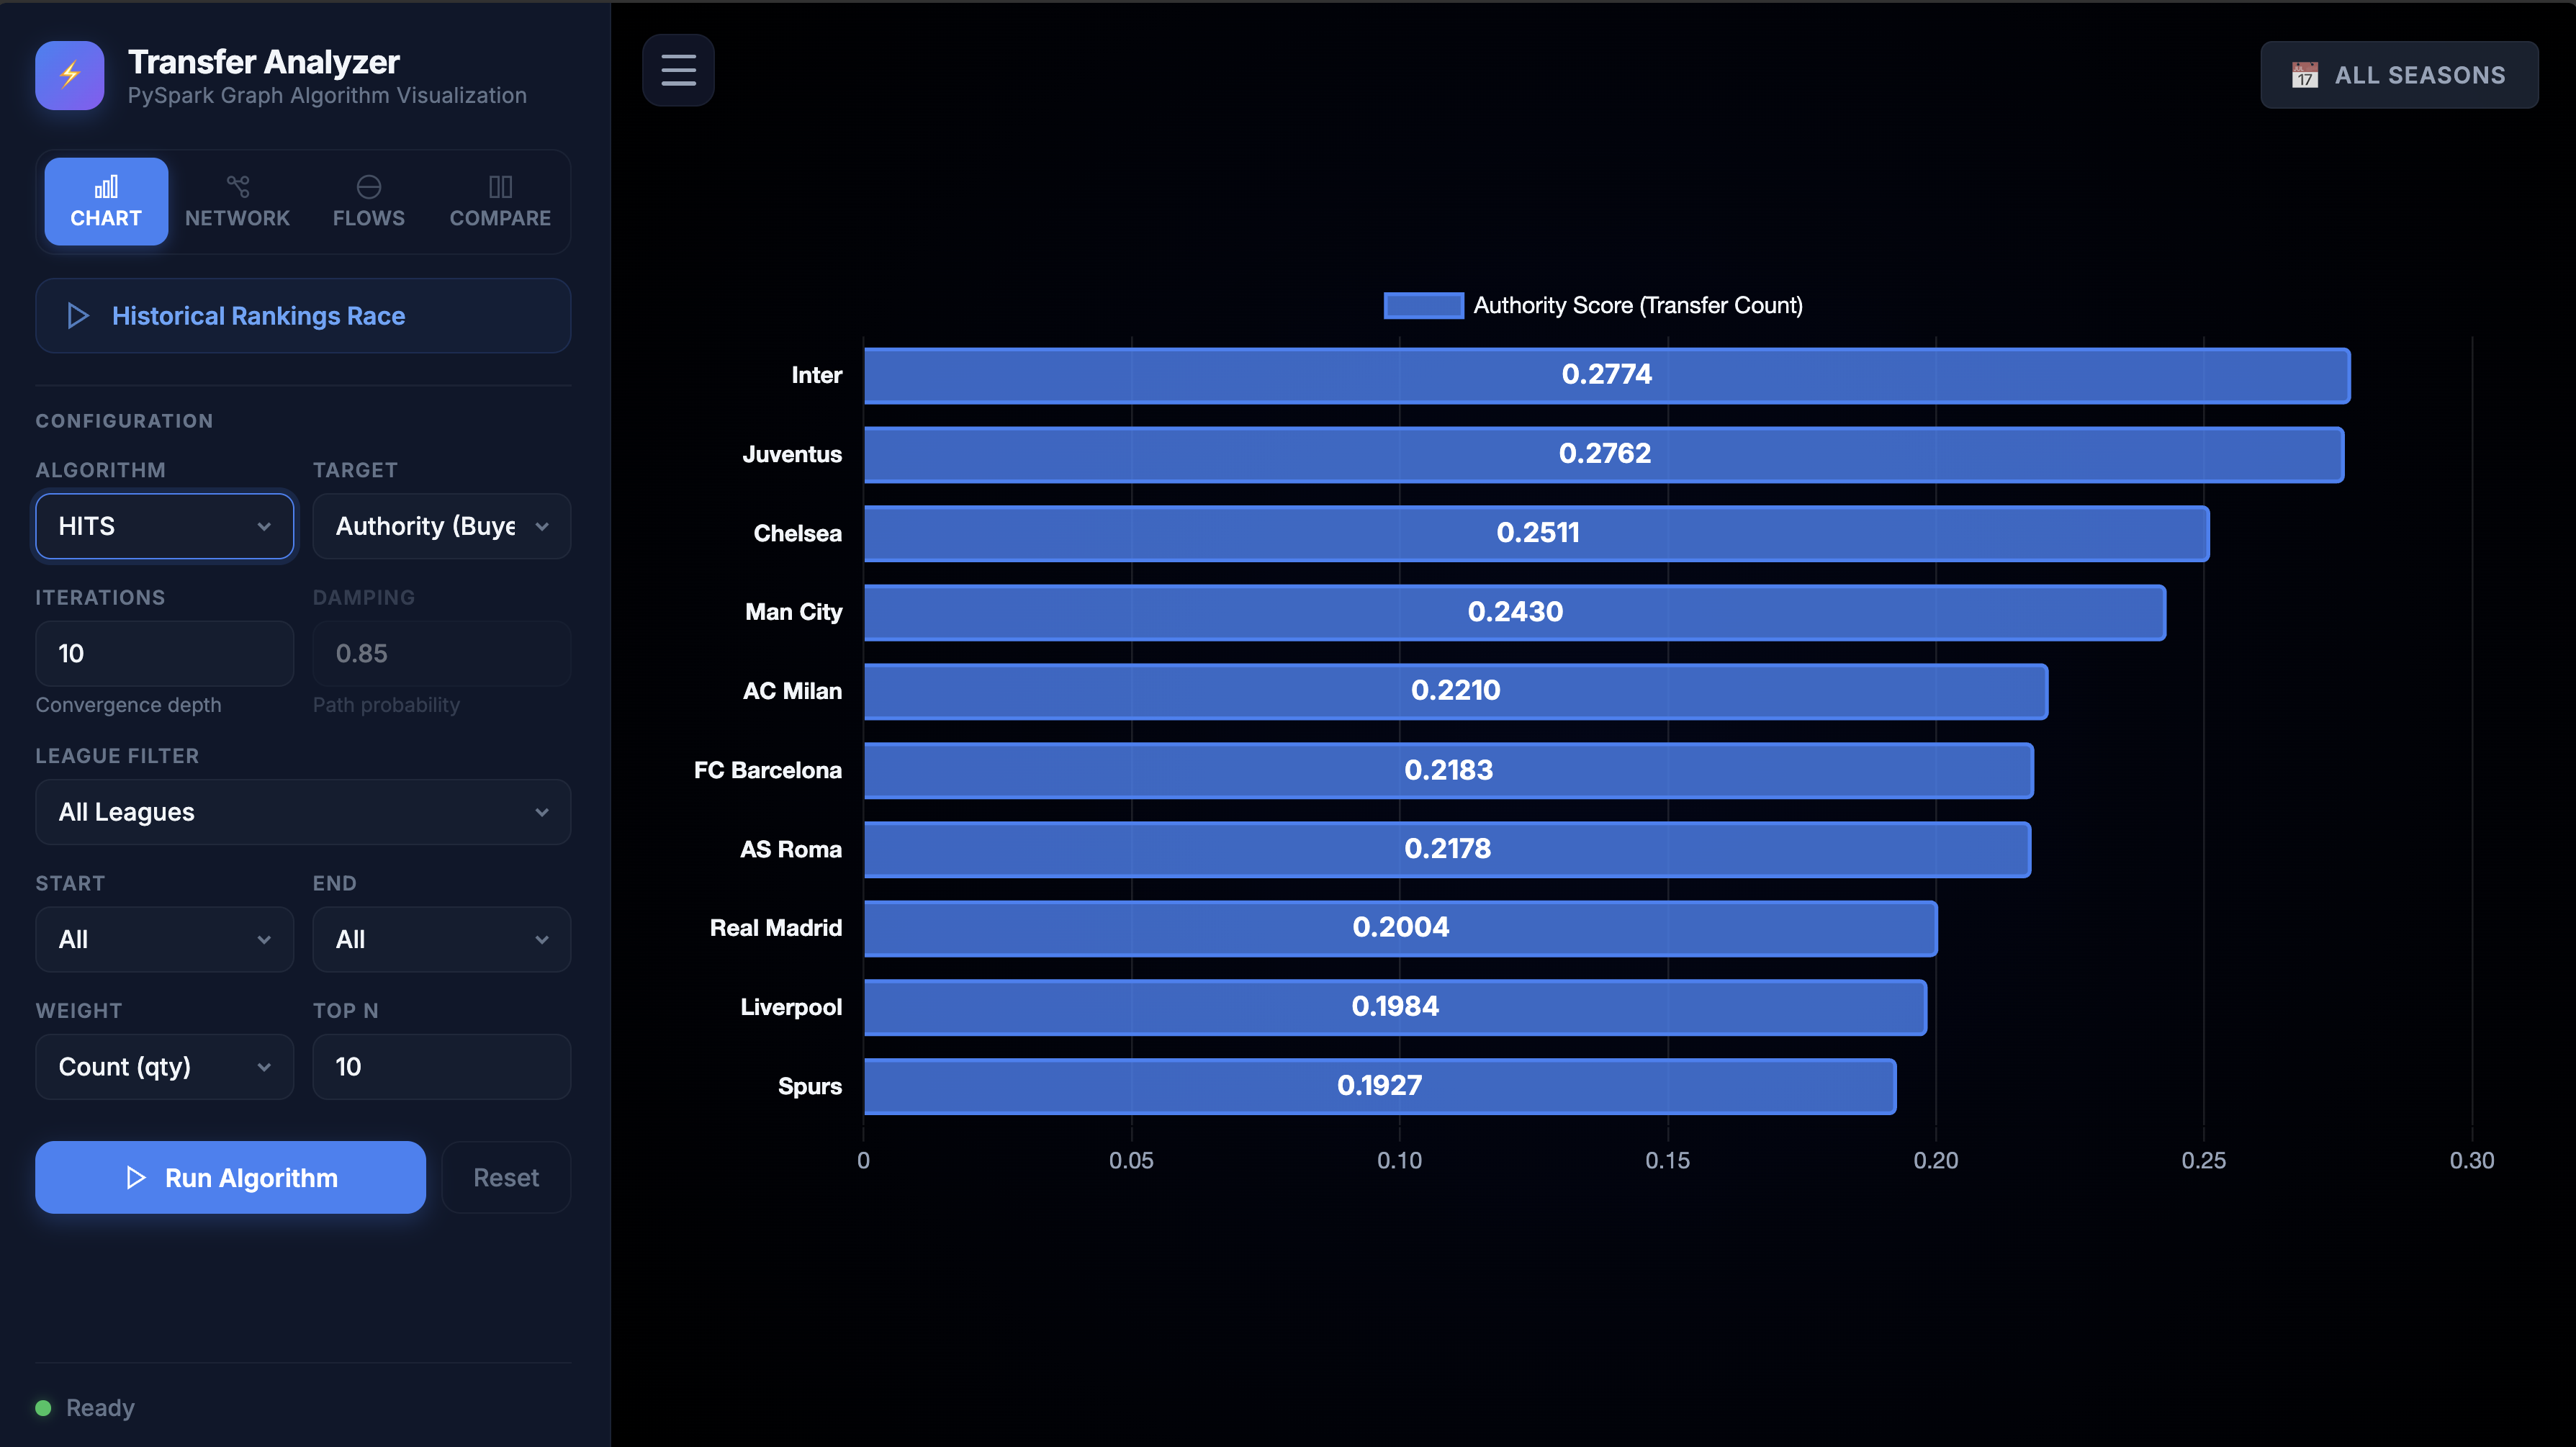
\includegraphics[width=1.0\textwidth]{Figures/ui_authority_buyers_hits_count.png}
    \caption{Application view for Top 10 Authority Buyers HITS (Count Weighted)}
    \label{fig:ui_authority_buyers_hits_count}

    \vspace{1.5em}
    
    \begin{tabular}{|l|l|r|}
\hline
\textbf{Rank} & \textbf{Club} & \textbf{Score} \\
\hline
1 & Inter & 0.2774 \\
2 & Juventus & 0.2762 \\
3 & Chelsea & 0.2511 \\
4 & Man City & 0.2430 \\
5 & AC Milan & 0.2210 \\
6 & FC Barcelona & 0.2183 \\
7 & AS Roma & 0.2178 \\
8 & Real Madrid & 0.2004 \\
9 & Liverpool & 0.1984 \\
10 & Spurs & 0.1927 \\
\hline
\end{tabular}
    \captionof{table}{Top 10 Authority Buyers HITS - Count Weighted}
    \label{tab:top_10_authority_buyers_hits___count_weighted}
\end{figure}

% Top 10 Sellers PageRank - Count Weighted
\begin{figure}[H]
    \centering
    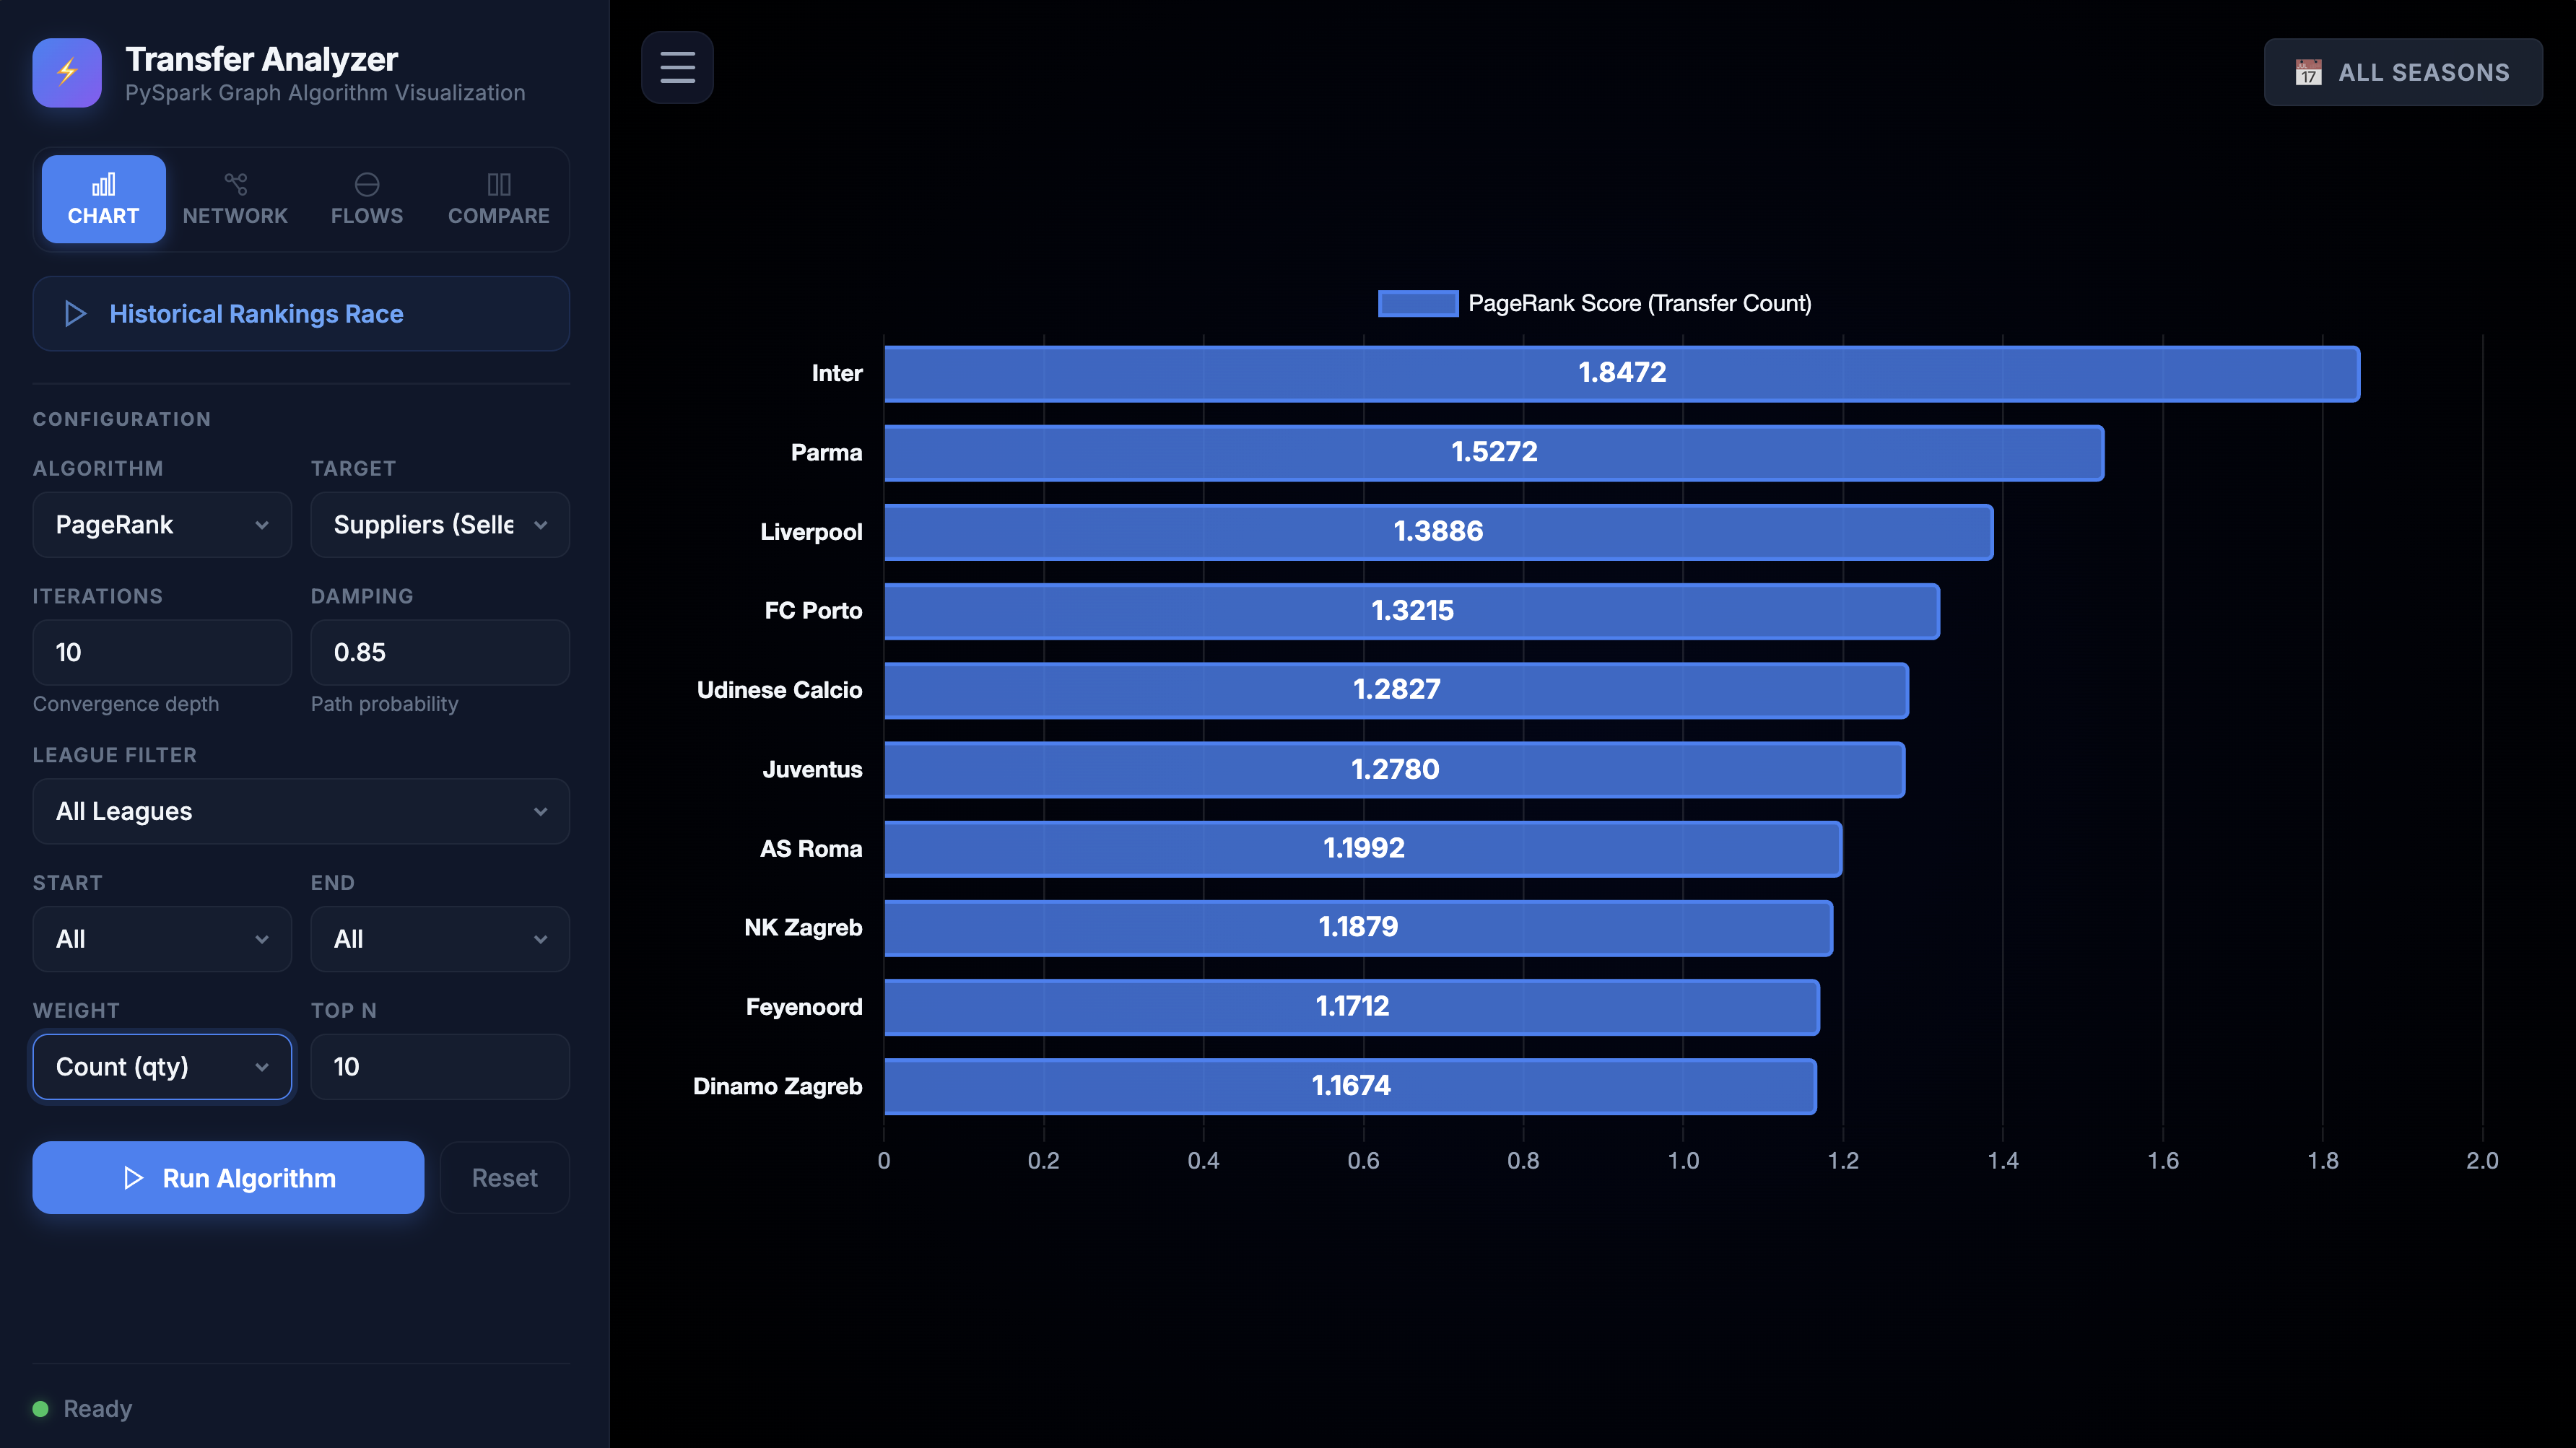
\includegraphics[width=1.0\textwidth]{Figures/ui_sellers_pagerank_count.png}
    \caption{Application view for Top 10 Sellers PageRank (Count Weighted)}
    \label{fig:ui_sellers_pagerank_count}

    \vspace{1.5em}
    
    \begin{tabular}{|l|l|r|}
\hline
\textbf{Rank} & \textbf{Club} & \textbf{Score} \\
\hline
1 & Inter & 1.8472 \\
2 & Parma & 1.5272 \\
3 & Liverpool & 1.3886 \\
4 & FC Porto & 1.3215 \\
5 & Udinese Calcio & 1.2827 \\
6 & Juventus & 1.2780 \\
7 & AS Roma & 1.1992 \\
8 & NK Zagreb & 1.1879 \\
9 & Feyenoord & 1.1712 \\
10 & Dinamo Zagreb & 1.1674 \\
\hline
\end{tabular}
    \captionof{table}{Top 10 Sellers PageRank - Count Weighted}
    \label{tab:top_10_sellers_pagerank___count_weighted}
\end{figure}

% Top 10 Hubs Sellers HITS - Count Weighted
\begin{figure}[H]
    \centering
    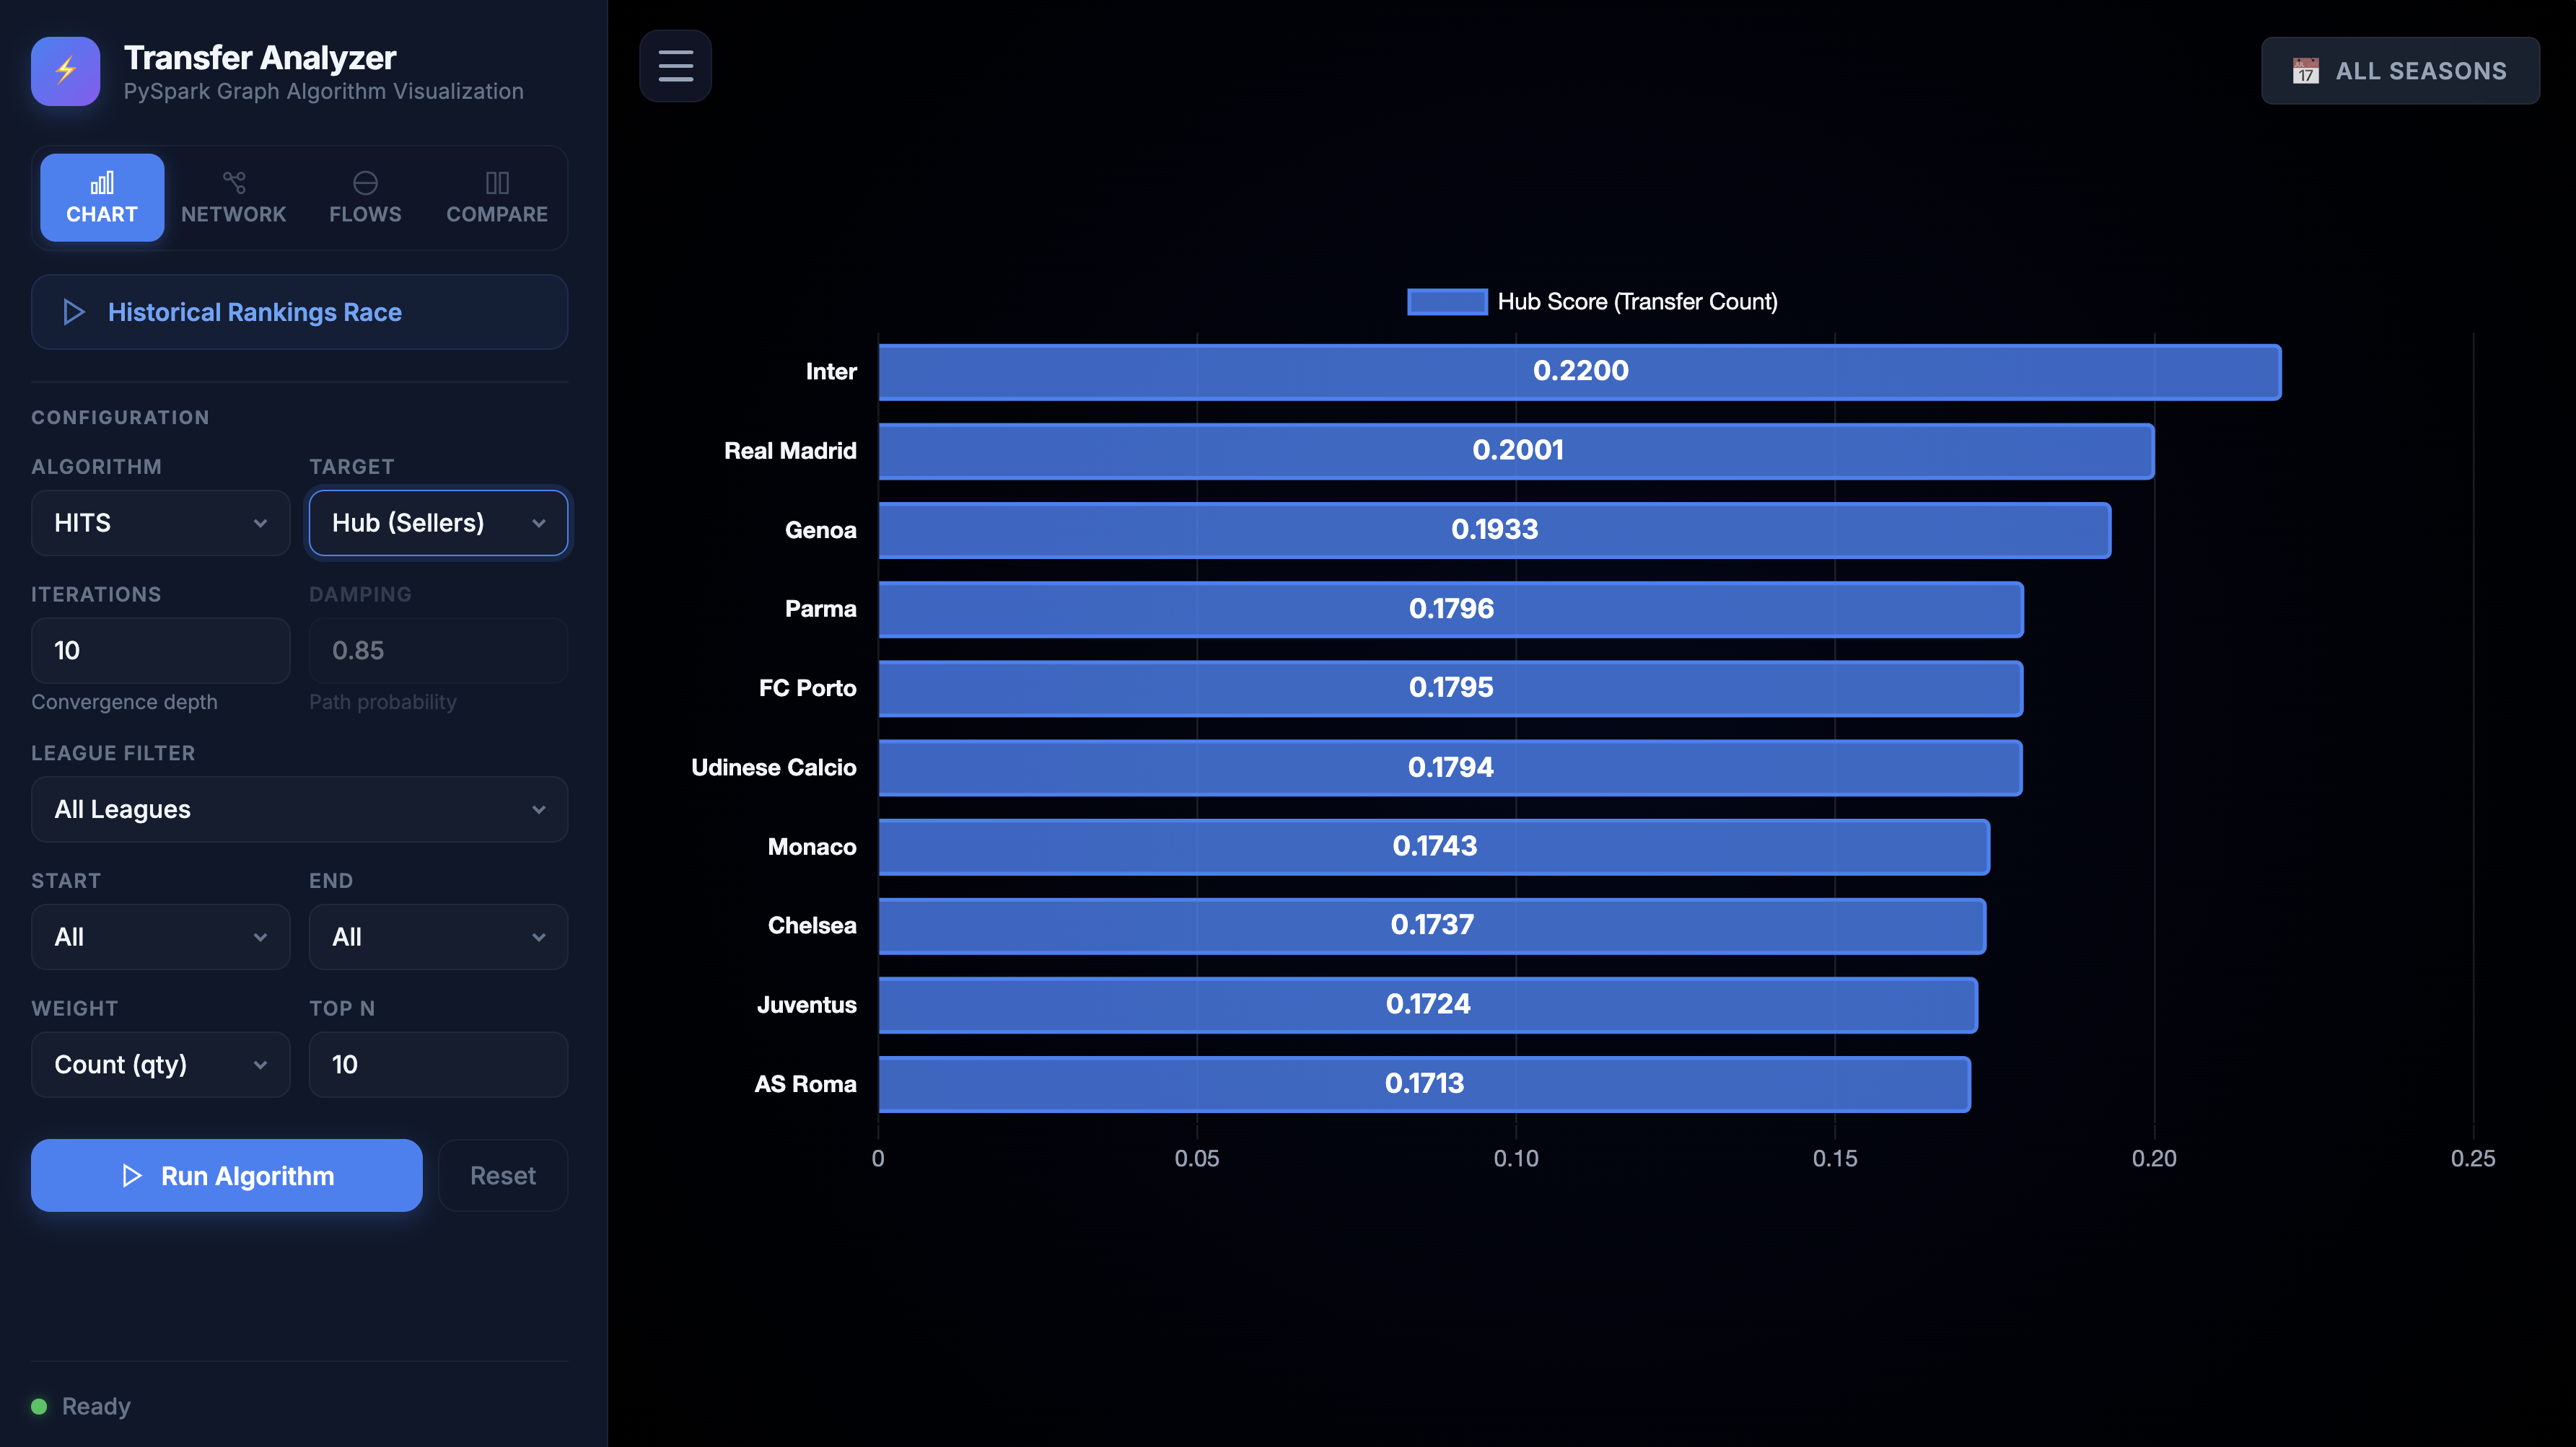
\includegraphics[width=1.0\textwidth]{Figures/ui_hubs_sellers_hits_count.png}
    \caption{Application view for Top 10 Hubs Sellers HITS (Count Weighted)}
    \label{fig:ui_hubs_sellers_hits_count}

    \vspace{1.5em}
    
    \begin{tabular}{|l|l|r|}
\hline
\textbf{Rank} & \textbf{Club} & \textbf{Score} \\
\hline
1 & Inter & 0.2200 \\
2 & Real Madrid & 0.2001 \\
3 & Genoa & 0.1933 \\
4 & Parma & 0.1796 \\
5 & FC Porto & 0.1795 \\
6 & Udinese Calcio & 0.1794 \\
7 & Monaco & 0.1743 \\
8 & Chelsea & 0.1737 \\
9 & Juventus & 0.1724 \\
10 & AS Roma & 0.1713 \\
\hline
\end{tabular}
    \captionof{table}{Top 10 Hubs Sellers HITS - Count Weighted}
    \label{tab:top_10_hubs_sellers_hits___count_weighted}
\end{figure}

The count-weighted results strongly contrast with the fee-weighted results, particularly for HITS analysis. Under a count-based interpretation, Italian clubs like Inter, Juventus, Parma, and AS Roma emerge significantly more prominent as both authorities and hubs. This indicates a high frequency of transfer interactions within the Italian market and across Europe, regardless of the individual transfer fees involved. The hub/authority duality confirms that these clubs maintain central structural roles precisely because they acquire and supply players repeatedly, serving as key operational nodes in the talent exchange network.

%=============================================================
\section{Effect of League and Season Filters}
\label{sec:results_filters}

\subsection{League-Specific Analysis}
\label{subsec:results_leagues}

Applying league filters changes the graph topology substantially. Instead of analyzing the global transfer ecosystem, the user can isolate an intra-league market and observe how centrality behaves within a narrower competitive environment.

This is methodologically important because a club's global importance does not necessarily imply equivalent importance within a specific league-only context. A club may be highly central in the broader European transfer network while appearing less dominant when only domestic league interactions are considered. Conversely, clubs that play an active role within a league may become more visible once global giants are excluded.

\subsection{Season-Range Analysis}
\label{subsec:results_seasons}

Season filters provide a temporal lens through which ranking behavior can be examined. Restricting the graph to specific years changes both the set of active edges and the balance of influence among clubs. This makes it possible to study how transfer-market centrality evolves over time.

Temporal filtering is particularly important for football, where club influence is not static. Management changes, financial conditions, sporting success, and regulatory shifts can all alter a club's transfer behavior. The season-range feature therefore transforms the study from a purely static graph analysis into a temporally aware investigation of market dynamics.


%=============================================================
\section{Visualization-Based Interpretation}
\label{sec:results_visualization}

The results of the thesis are not interpreted solely through raw scores. The \textit{Transfer Analyzer} provides several analytical views, each contributing differently to the understanding of PageRank and HITS.

\subsection{Bar Chart View}
\label{subsec:results_bar_chart}

The ranked bar chart is the clearest view for comparing score magnitudes and ordinal positions. It allows immediate identification of the top clubs under each algorithm and is particularly useful for observing how the top-$N$ ordering changes when filters or parameters are modified.

For the thesis, the bar chart serves as the most direct presentation of ranking outcomes. It is especially effective when discussing which clubs dominate under fee-weighted versus count-weighted analysis, or when comparing buyer and seller roles.

\begin{figure}[H]
    \centering
    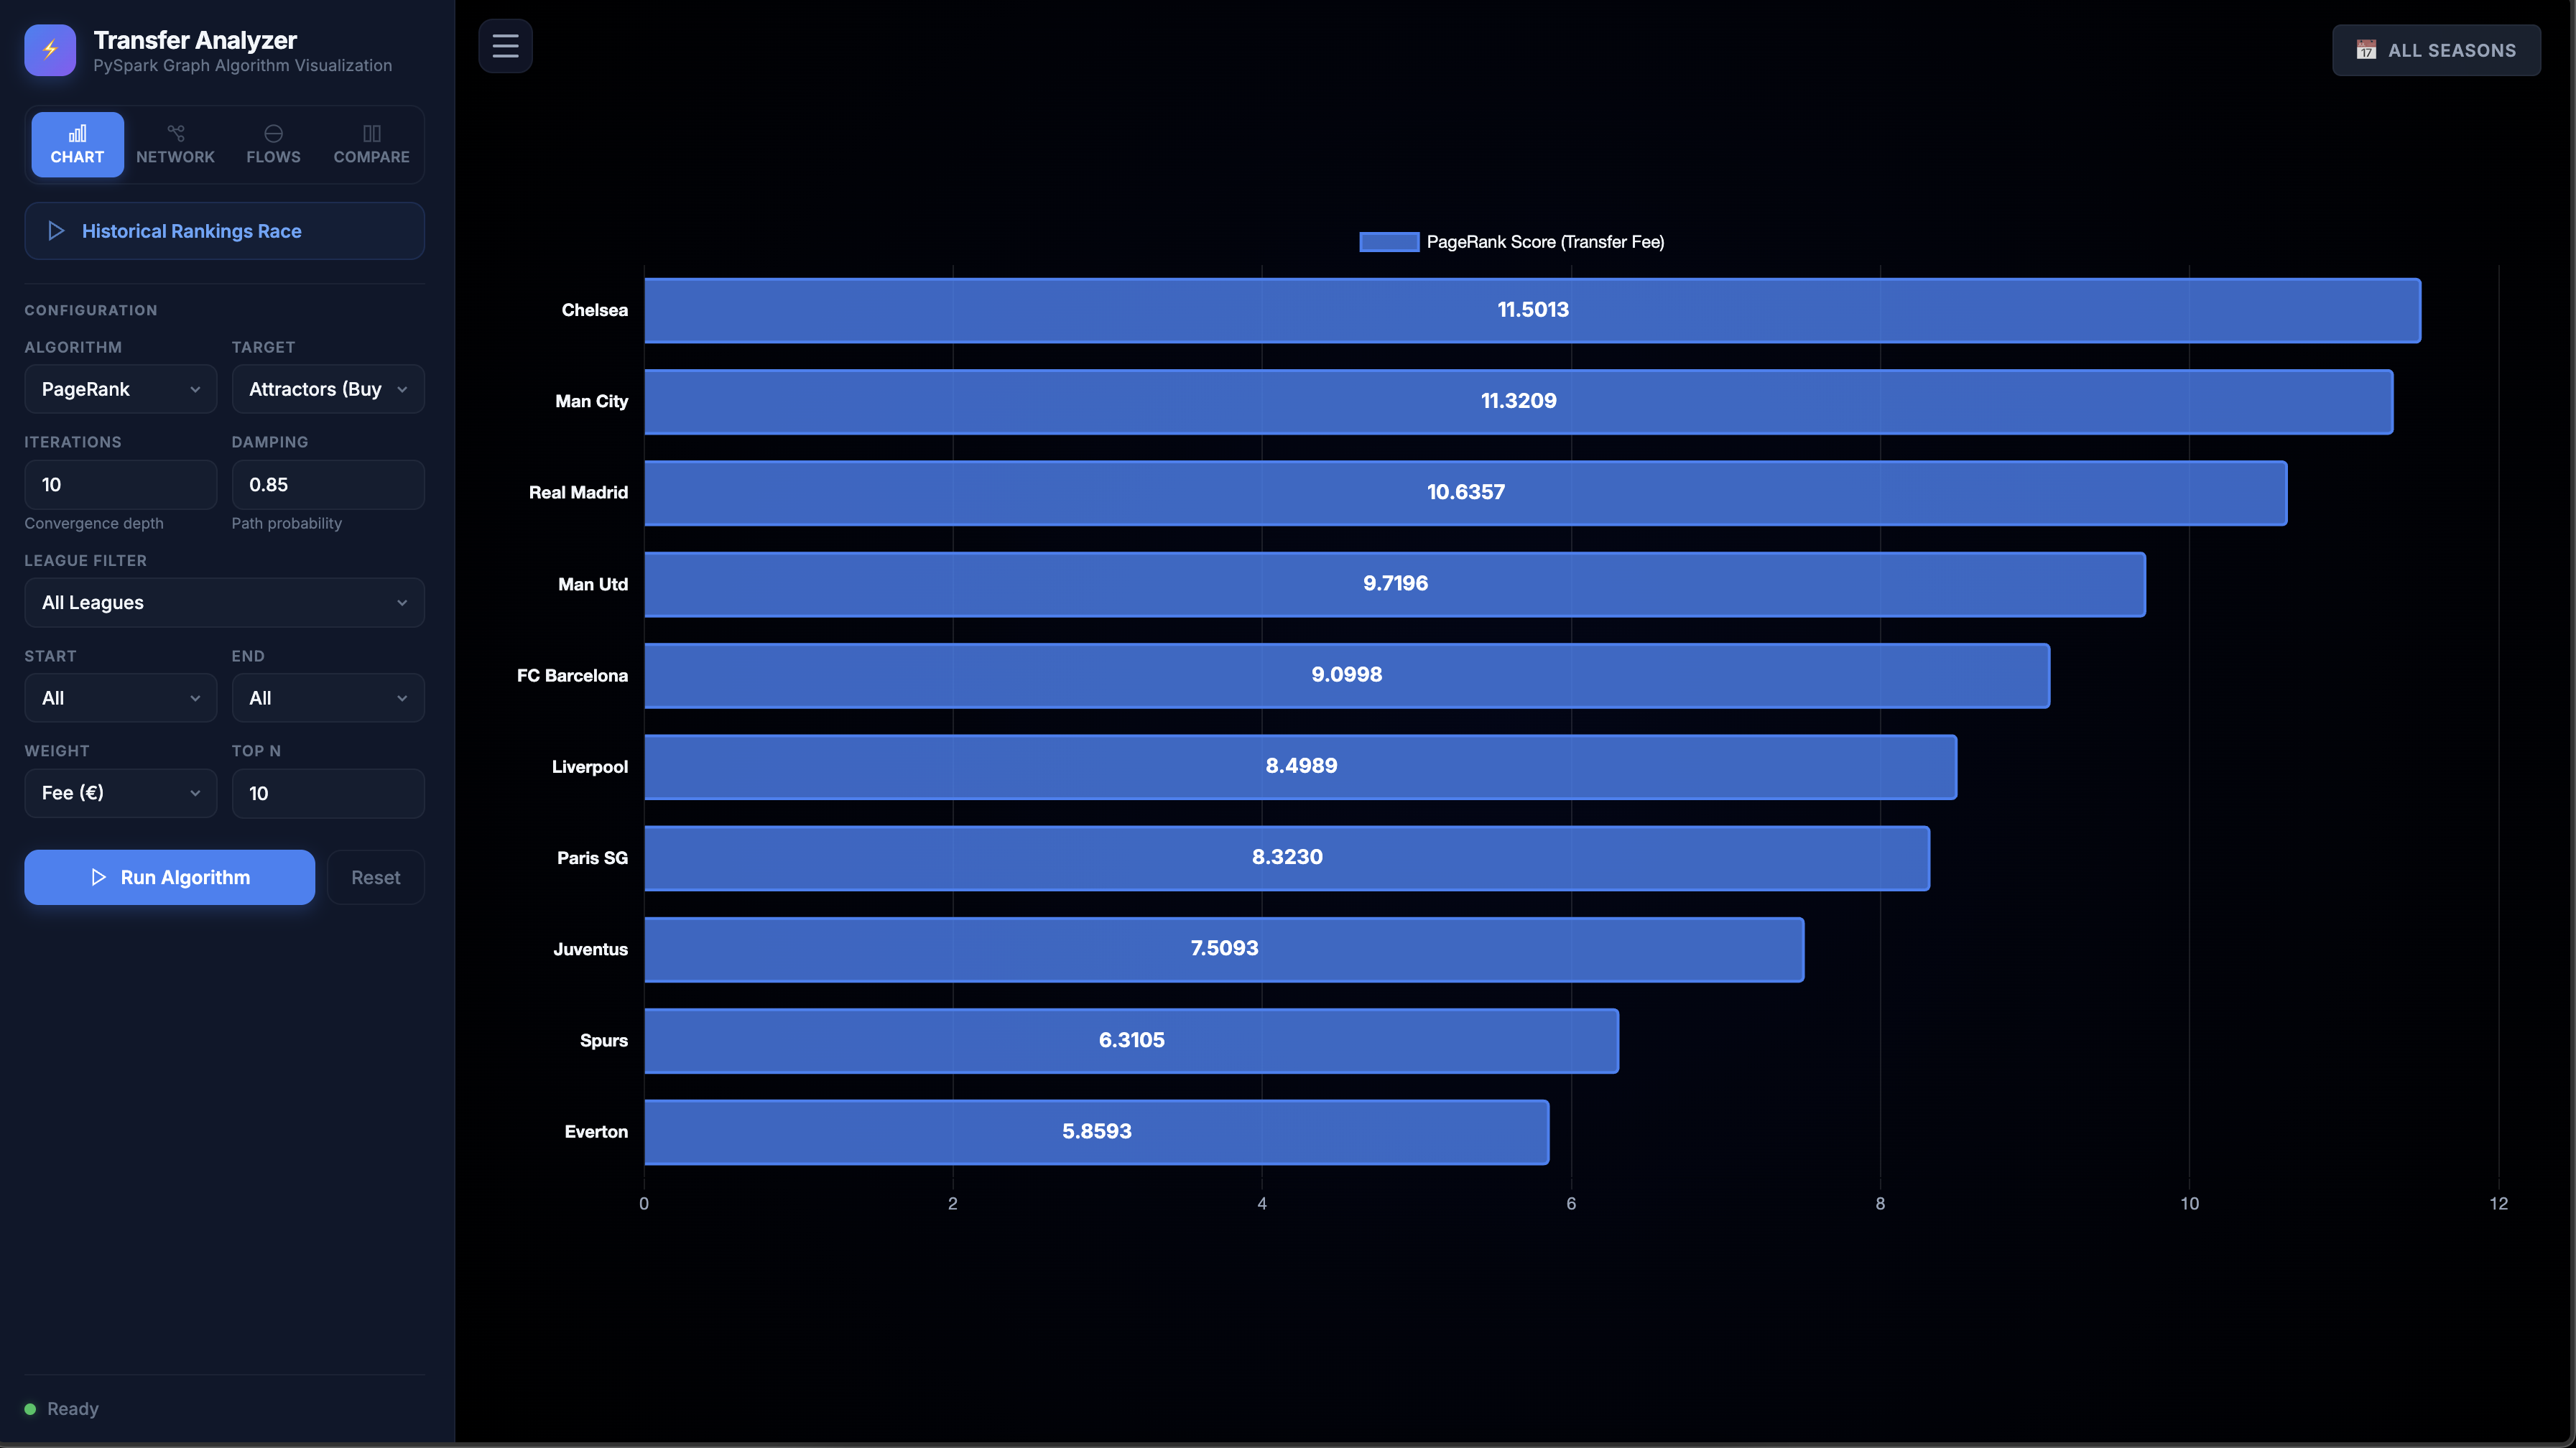
\includegraphics[width=1.0\textwidth]{Figures/ui_barchart.png}
    \caption{Interactive Bar Chart View displaying top-ranked clubs.}
    \label{fig:ui_barchart}
\end{figure}

\subsection{Network Graph View}
\label{subsec:results_network}

The network view complements the bar chart by showing the actual structural relations among clubs. While a ranked list indicates which clubs score highly, the network graph reveals how those clubs are connected through transfer edges.

This view is valuable because centrality scores gain more meaning when interpreted alongside the transfer relations that produced them. A club may rank highly due to receiving transfers from many peripheral clubs, from a few highly important clubs, or through dense interaction with other top-ranked clubs. The network graph helps distinguish among these possibilities visually.

\begin{figure}[H]
    \centering
    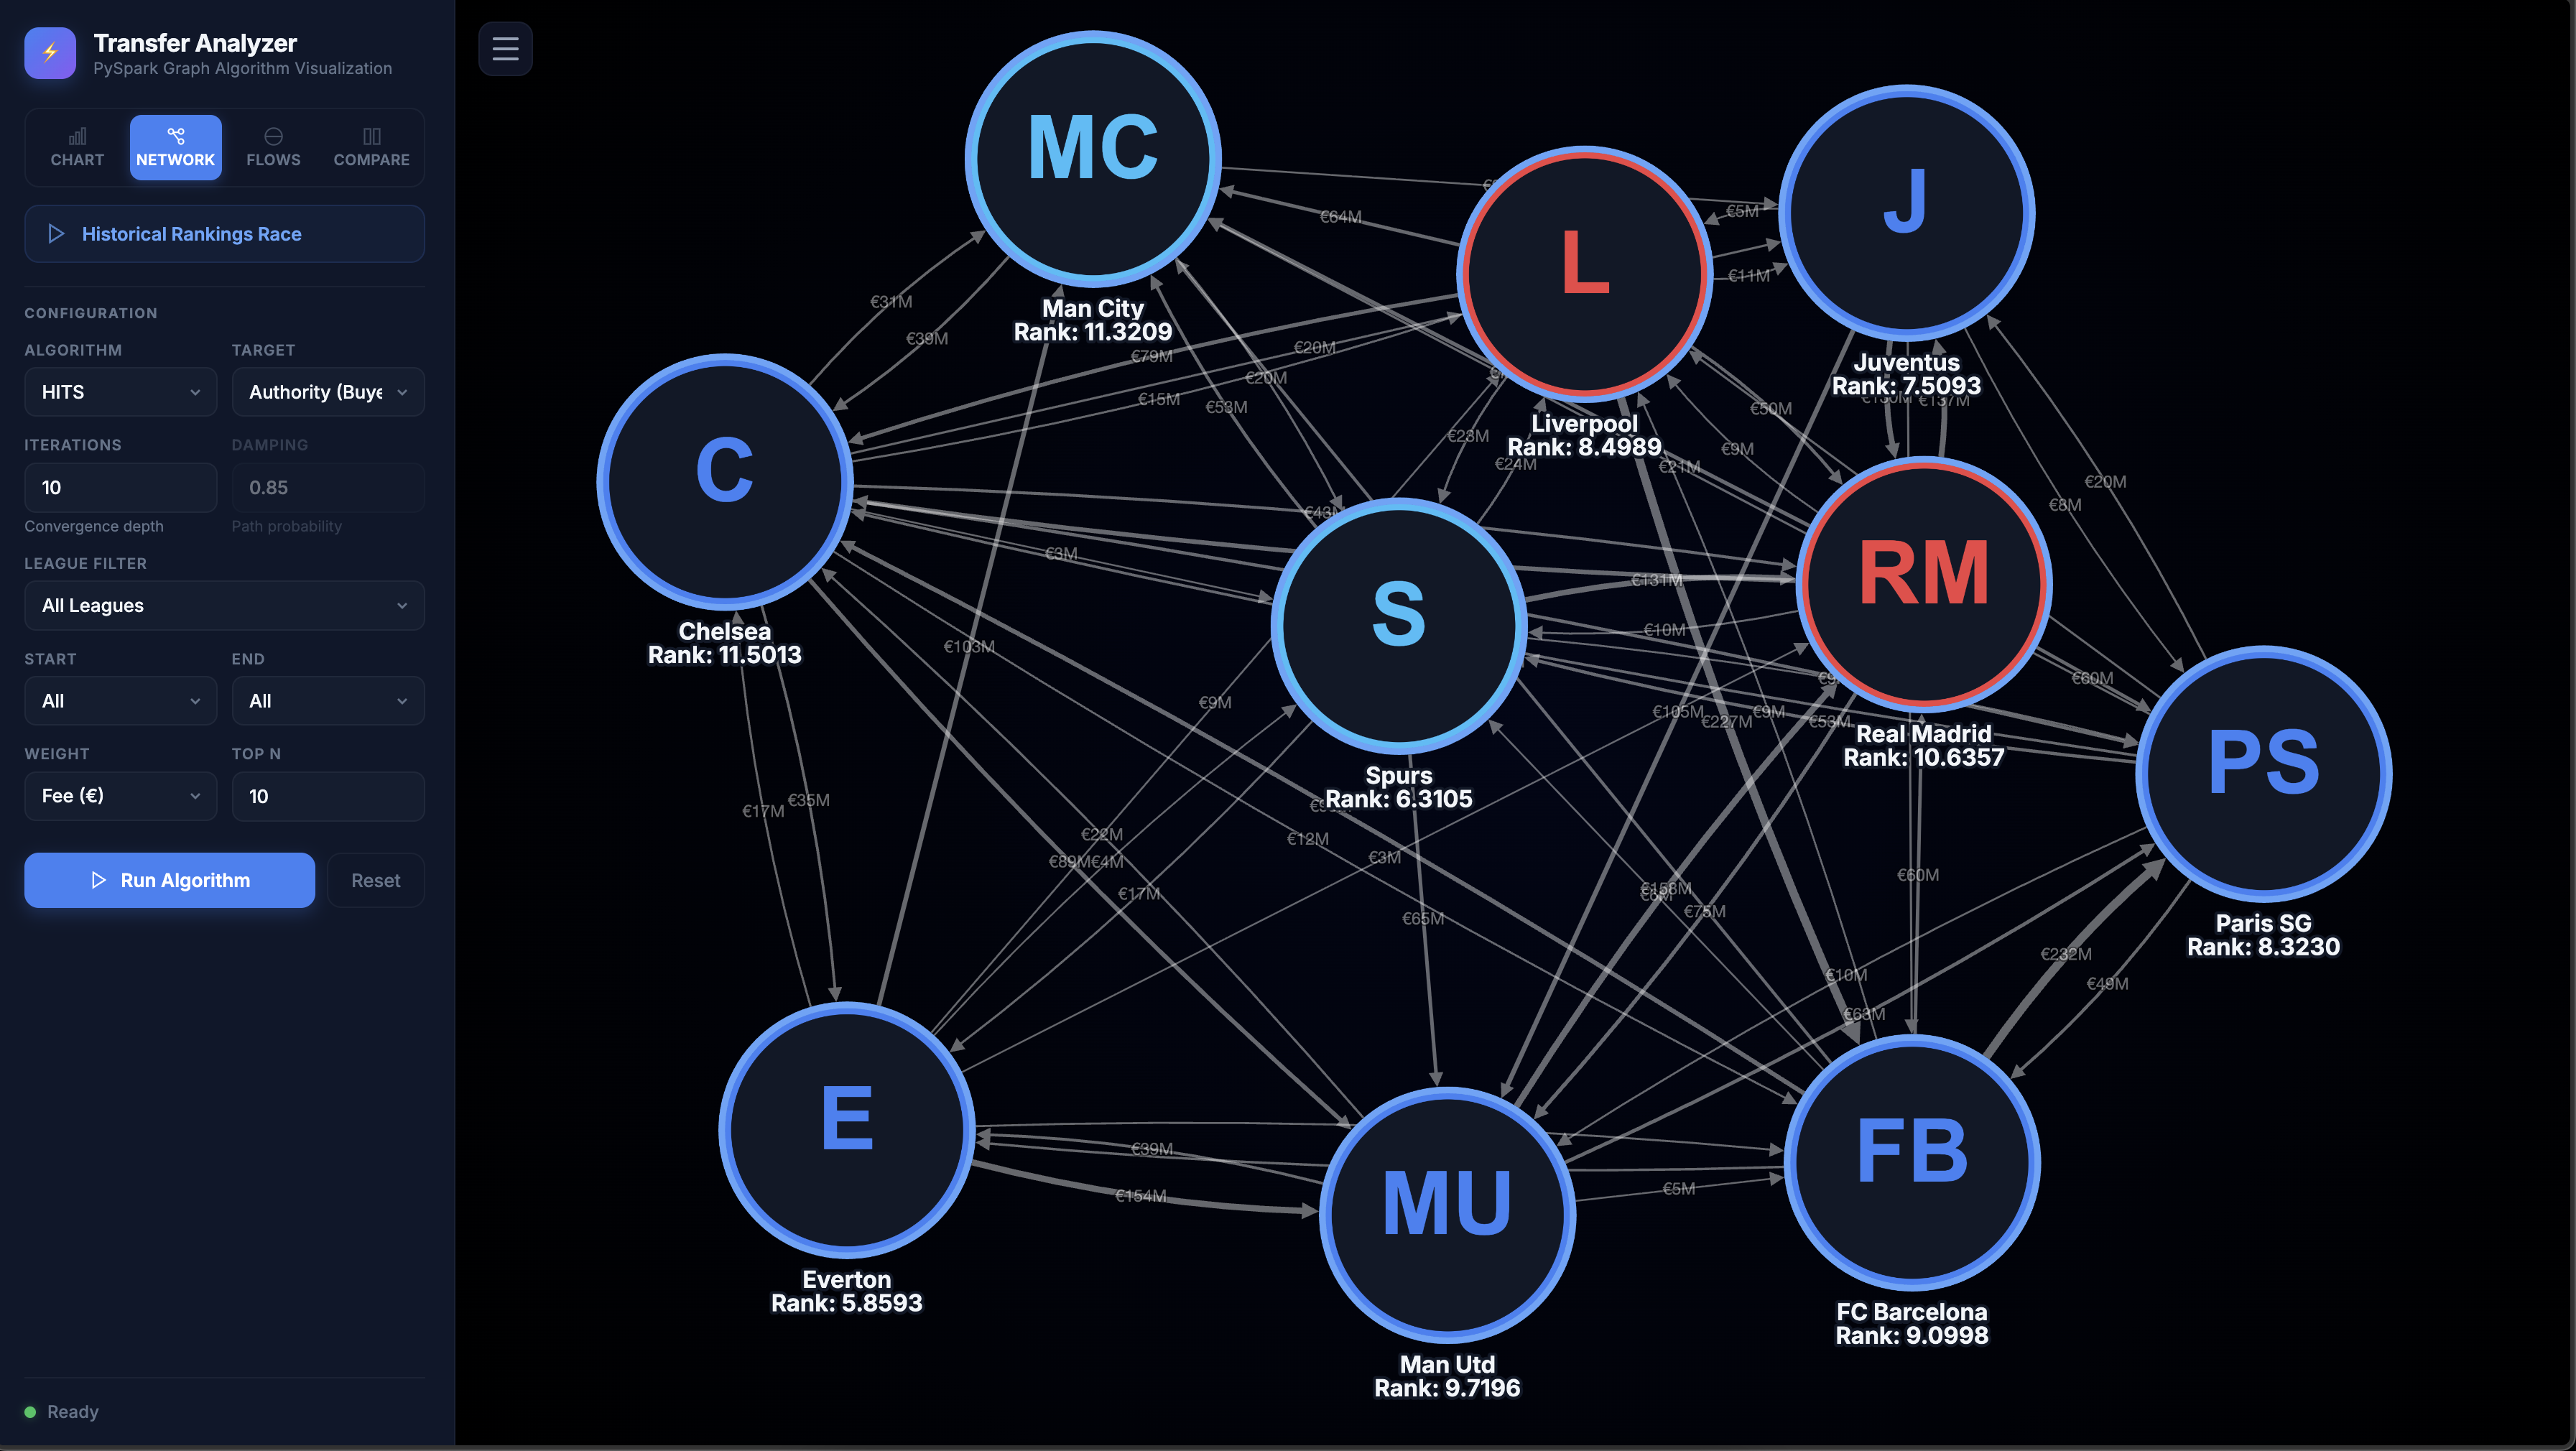
\includegraphics[width=1.0\textwidth]{Figures/ui_network.png}
    \caption{Network Graph View showing transfer relations between top clubs.}
    \label{fig:ui_network}
\end{figure}

%=============================================================
\subsection{League Flow View (Chord Diagram)}
\label{subsec:results_flow}

The flow-based view aggregates transfers at the league level rather than the club level, utilizing an interactive D3.js circular chord diagram. This is an important analytical extension because it shifts the perspective from individual club competition to broader market movement between leagues. The arc widths represent the exact financial volume (or frequency) of transfers, visually encoding the magnitude of movement.

In this mode, the thesis can interpret results not only in terms of club centrality but also in terms of macro-level transfer channels. Through interactive hover effects, it becomes possible to isolate specific league-to-league corridors and observe which leagues function as dominant suppliers, which act as major destinations, and how transfer value circulates across the football ecosystem.

\begin{figure}[H]
    \centering
    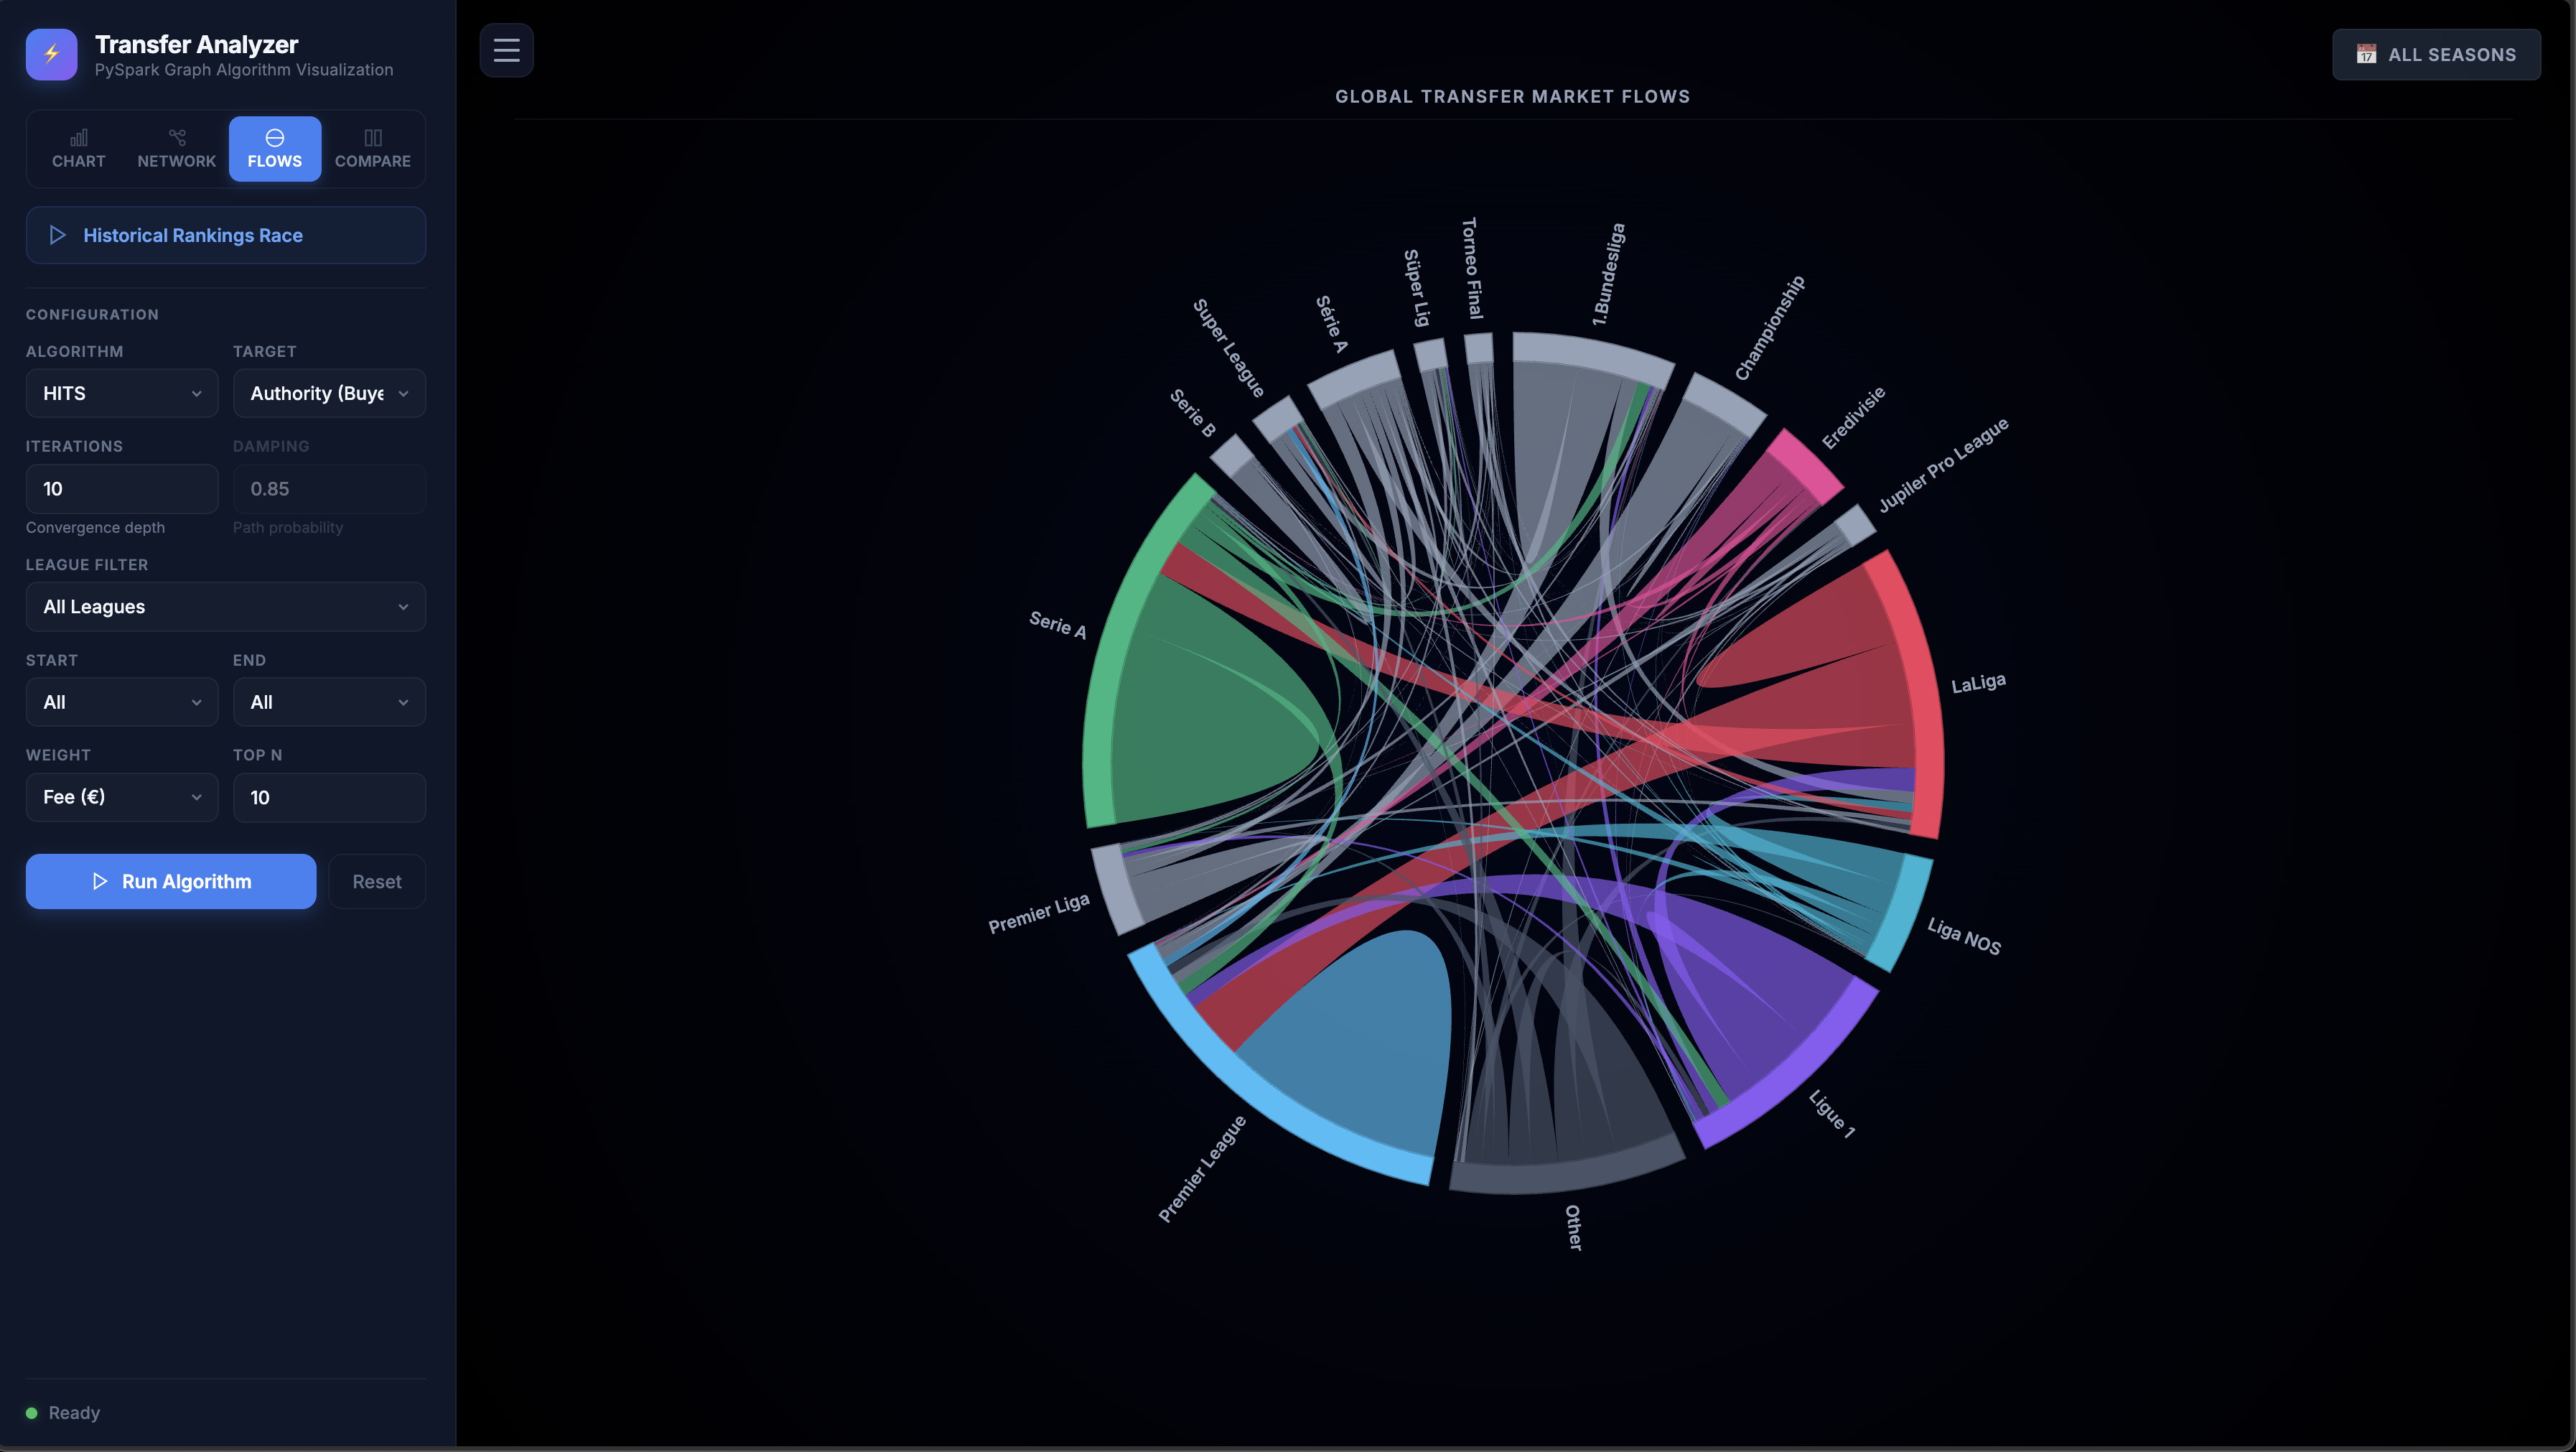
\includegraphics[width=1.0\textwidth]{Figures/ui_flow.png}
    \caption{League Flow View illustrating transfer volume between leagues.}
\end{figure}

\subsection{Compare Mode}
\label{subsec:results_compare}

The side-by-side compare mode is one of the most important contributions of the implemented system. It displays PageRank and HITS under identical filter conditions, allowing the user to inspect overlap and divergence directly.

This view supports the core research aim of the thesis: not simply to compute two algorithms independently, but to compare how they rank the same clubs on the same graph. Similar rankings suggest structural agreement, while different rankings indicate that the algorithms are emphasizing different notions of importance.

\begin{figure}[H]
    \centering
    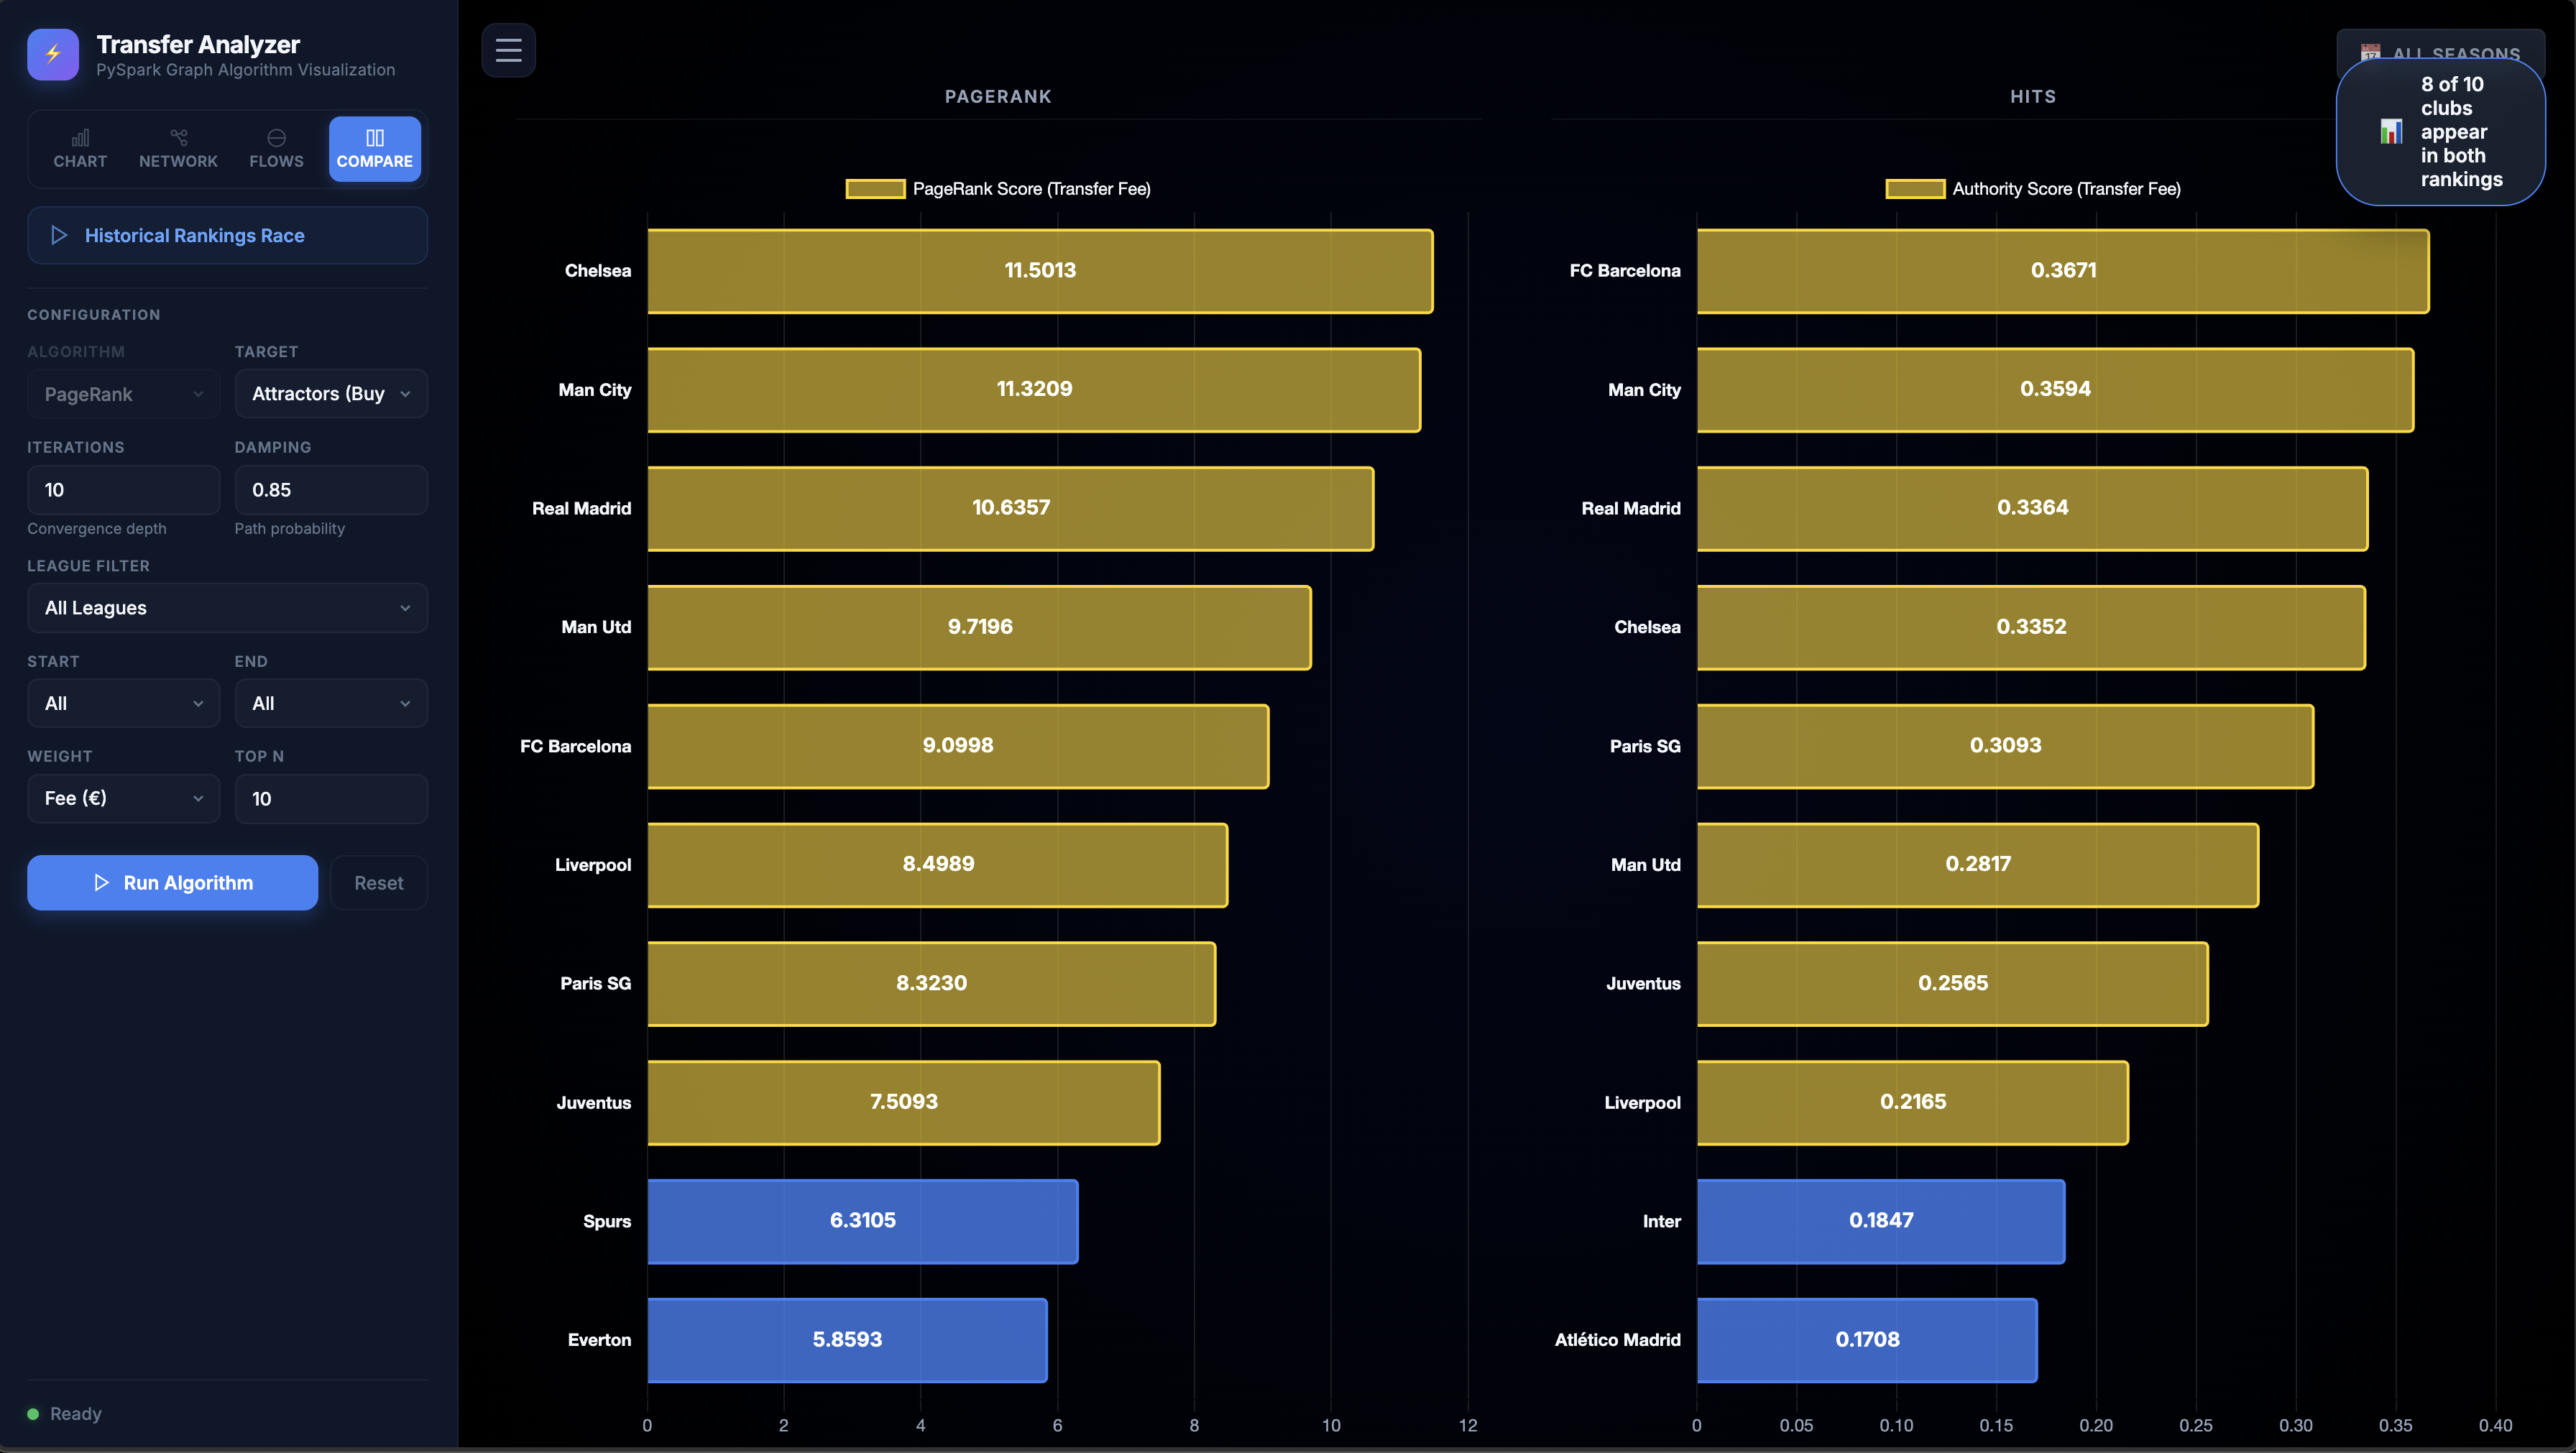
\includegraphics[width=1.0\textwidth]{Figures/ui_compare.png}
    \caption{Compare Mode displaying PageRank and HITS results side-by-side.}
    \label{fig:ui_compare}
\end{figure}

%=============================================================
\subsection{Historical Animated Bar Chart}
\label{subsec:results_historical}

The historical animated bar chart extends the analysis across time by showing how club rankings evolve season by season. Utilizing smooth D3.js transitions, this racing bar chart dynamically reorders clubs based on their computed scores for each season. Rather than presenting isolated static snapshots, this mode visualizes the dynamic rise, decline, and persistence of clubs in the transfer market.

This temporal mode is especially useful for identifying long-term patterns. Some clubs may remain consistently prominent across many seasons, indicating sustained market influence. Others may experience short-lived surges corresponding to specific financial periods, sporting projects, or transfer strategies. The animated view therefore transforms the results into a narrative of historical evolution rather than a single final ranking.

Furthermore, the implementation supports instantaneous switching between PageRank and HITS Authority algorithms during playback. Both models are pre-computed sequentially, allowing the user to pause the timeline at any specific year and toggle the algorithm. The visual interface immediately transitions the club bars to their new mathematical ranking for that exact season, providing a highly granular, frame-by-frame comparative analysis of algorithmic behavior.

\begin{figure}[H]
    \centering
    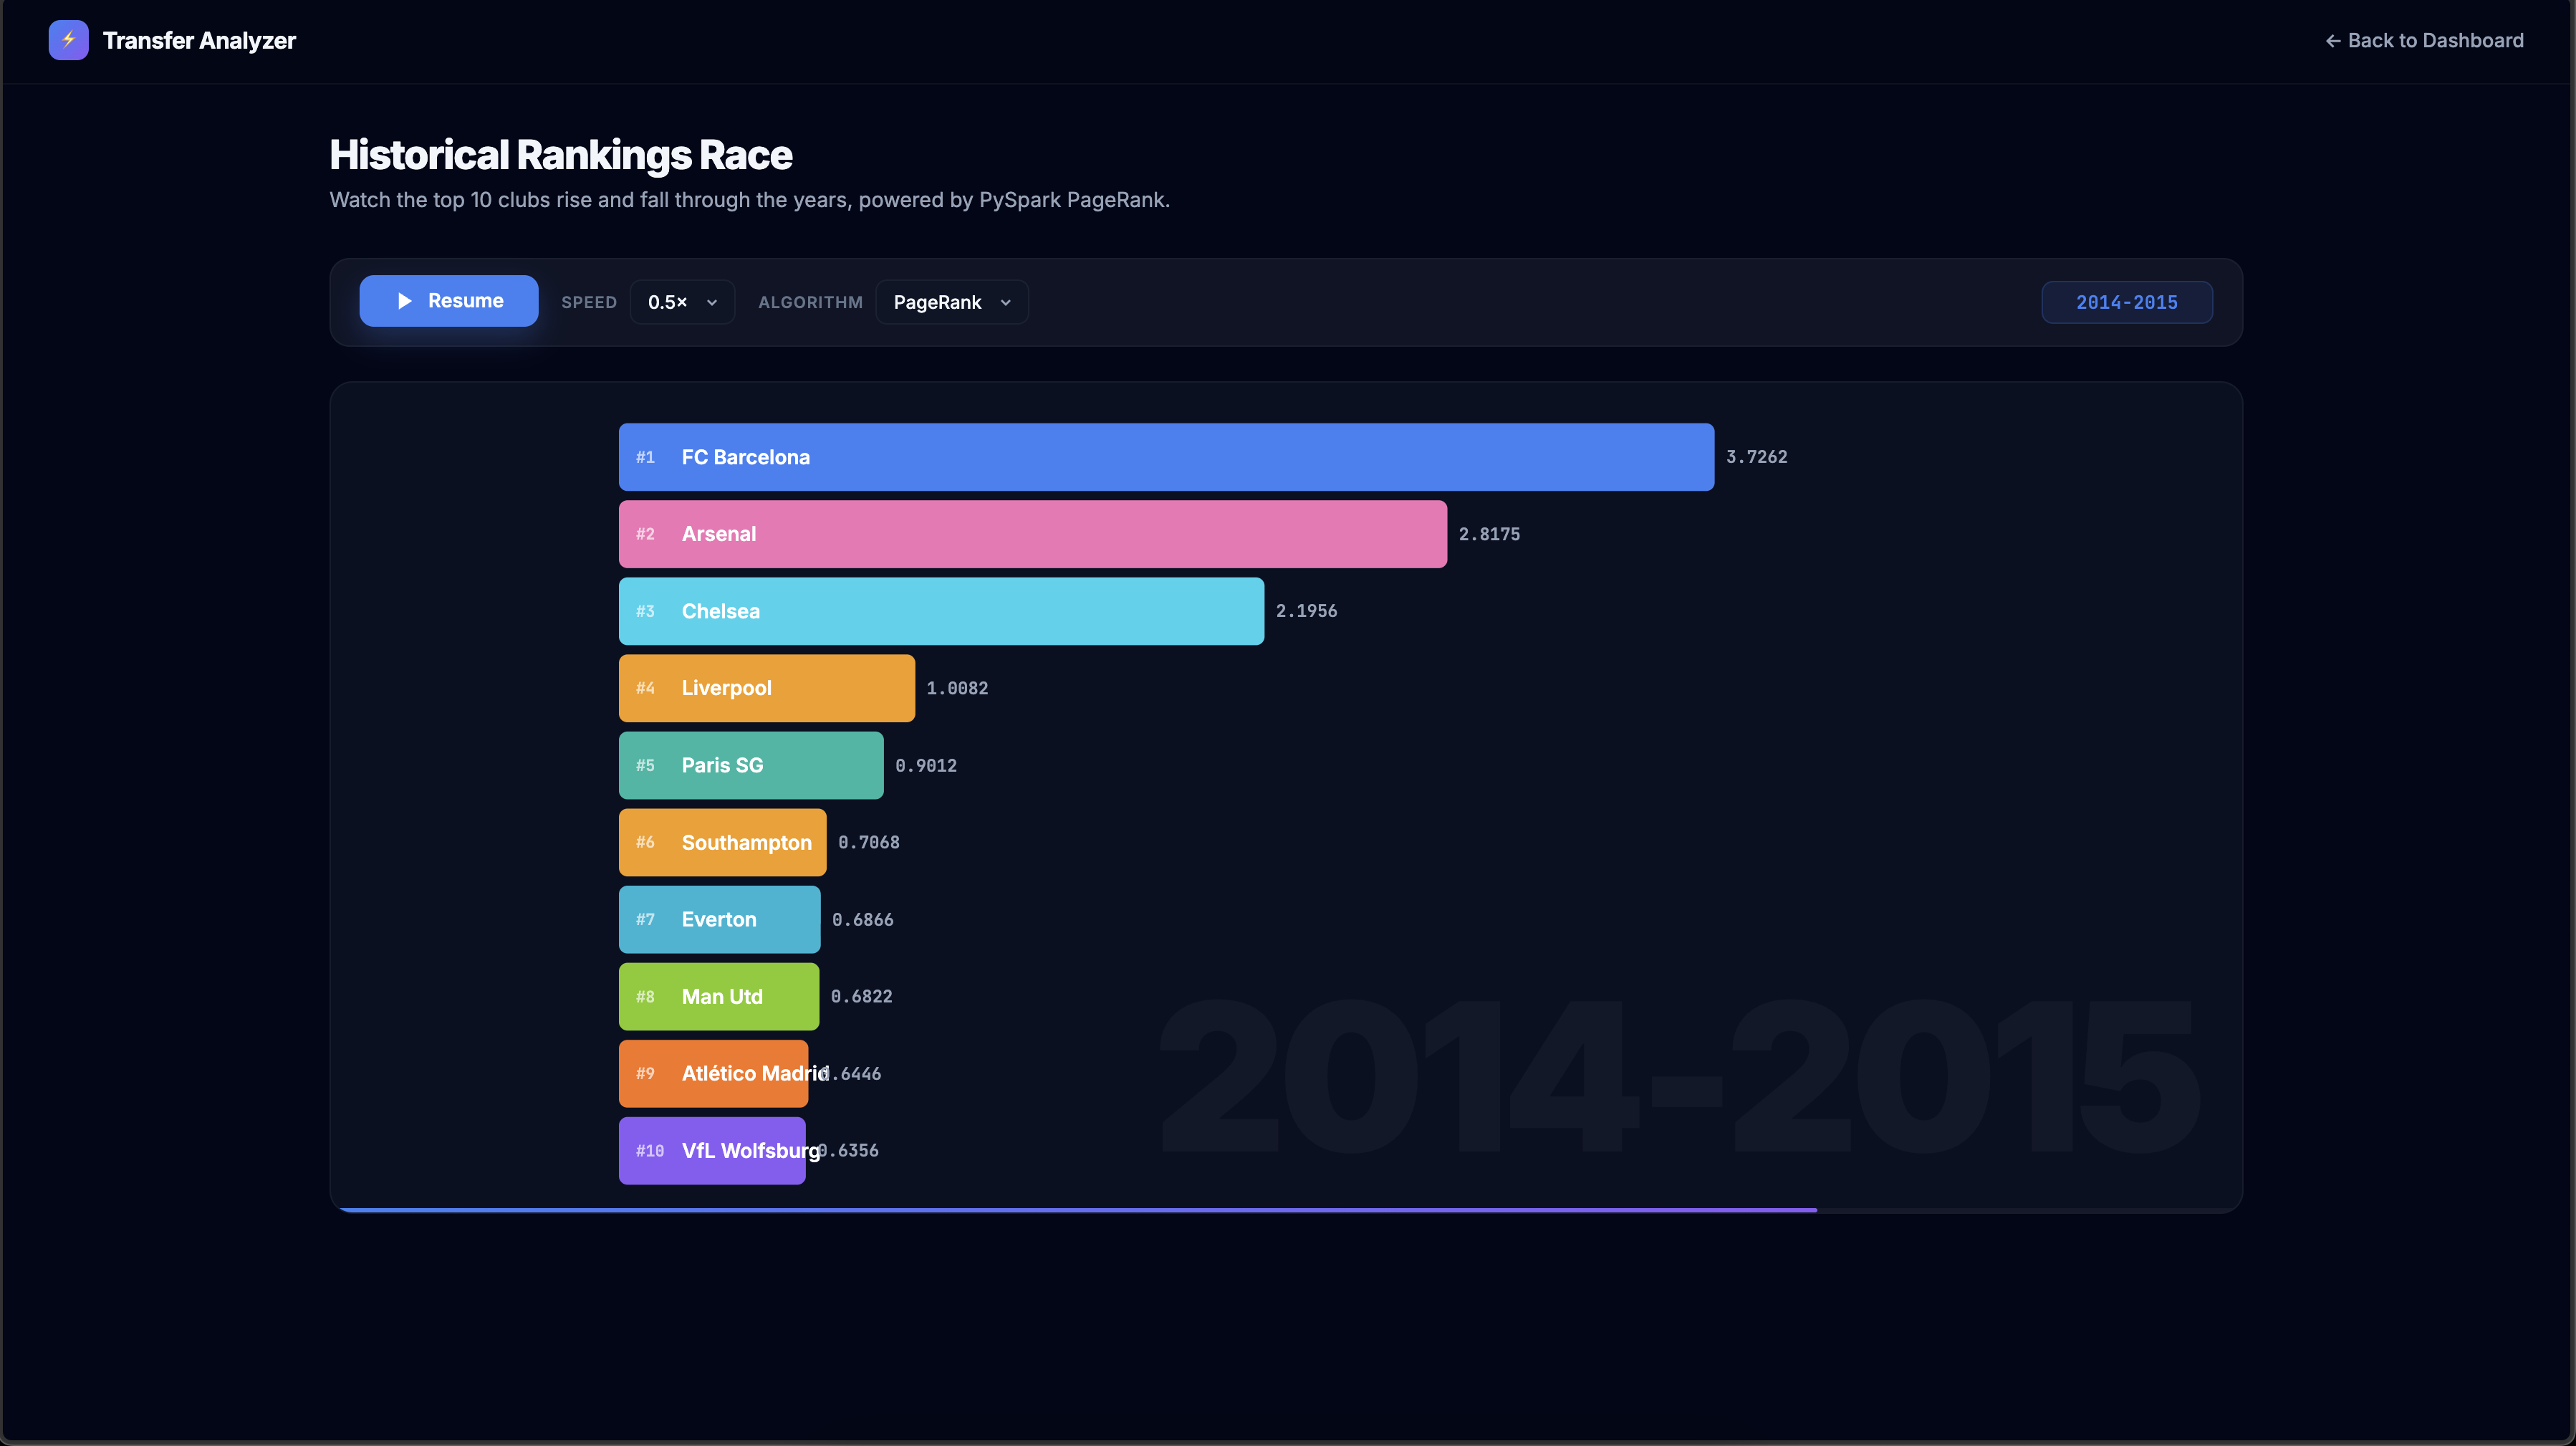
\includegraphics[width=1.0\textwidth]{Figures/ui_historical.png}
    \caption{Historical Animated Bar Chart tracking rankings across seasons.}
    \label{fig:ui_historical}
\end{figure}

\subsection{Transfer Details Panel}
\label{subsec:results_transfer_details}

To bridge the gap between macro-level graph algorithms and micro-level raw data verification, the \textit{Transfer Analyzer} includes an interactive transfer details popup. When a user clicks on any specific club's bar in the ranking chart, a panel opens displaying the exact incoming and outgoing transfers that constitute the club's score.

This feature is highly valuable from an analytical standpoint. It allows users to inspect whether a club's high PageRank or HITS score is the result of a few massive, high-value transfers or a large accumulation of smaller transfers. By exposing the underlying edges of the graph directly on demand, the system ensures transparency and reinforces the interpretability of the computed metrics.

\begin{figure}[H]
    \centering
    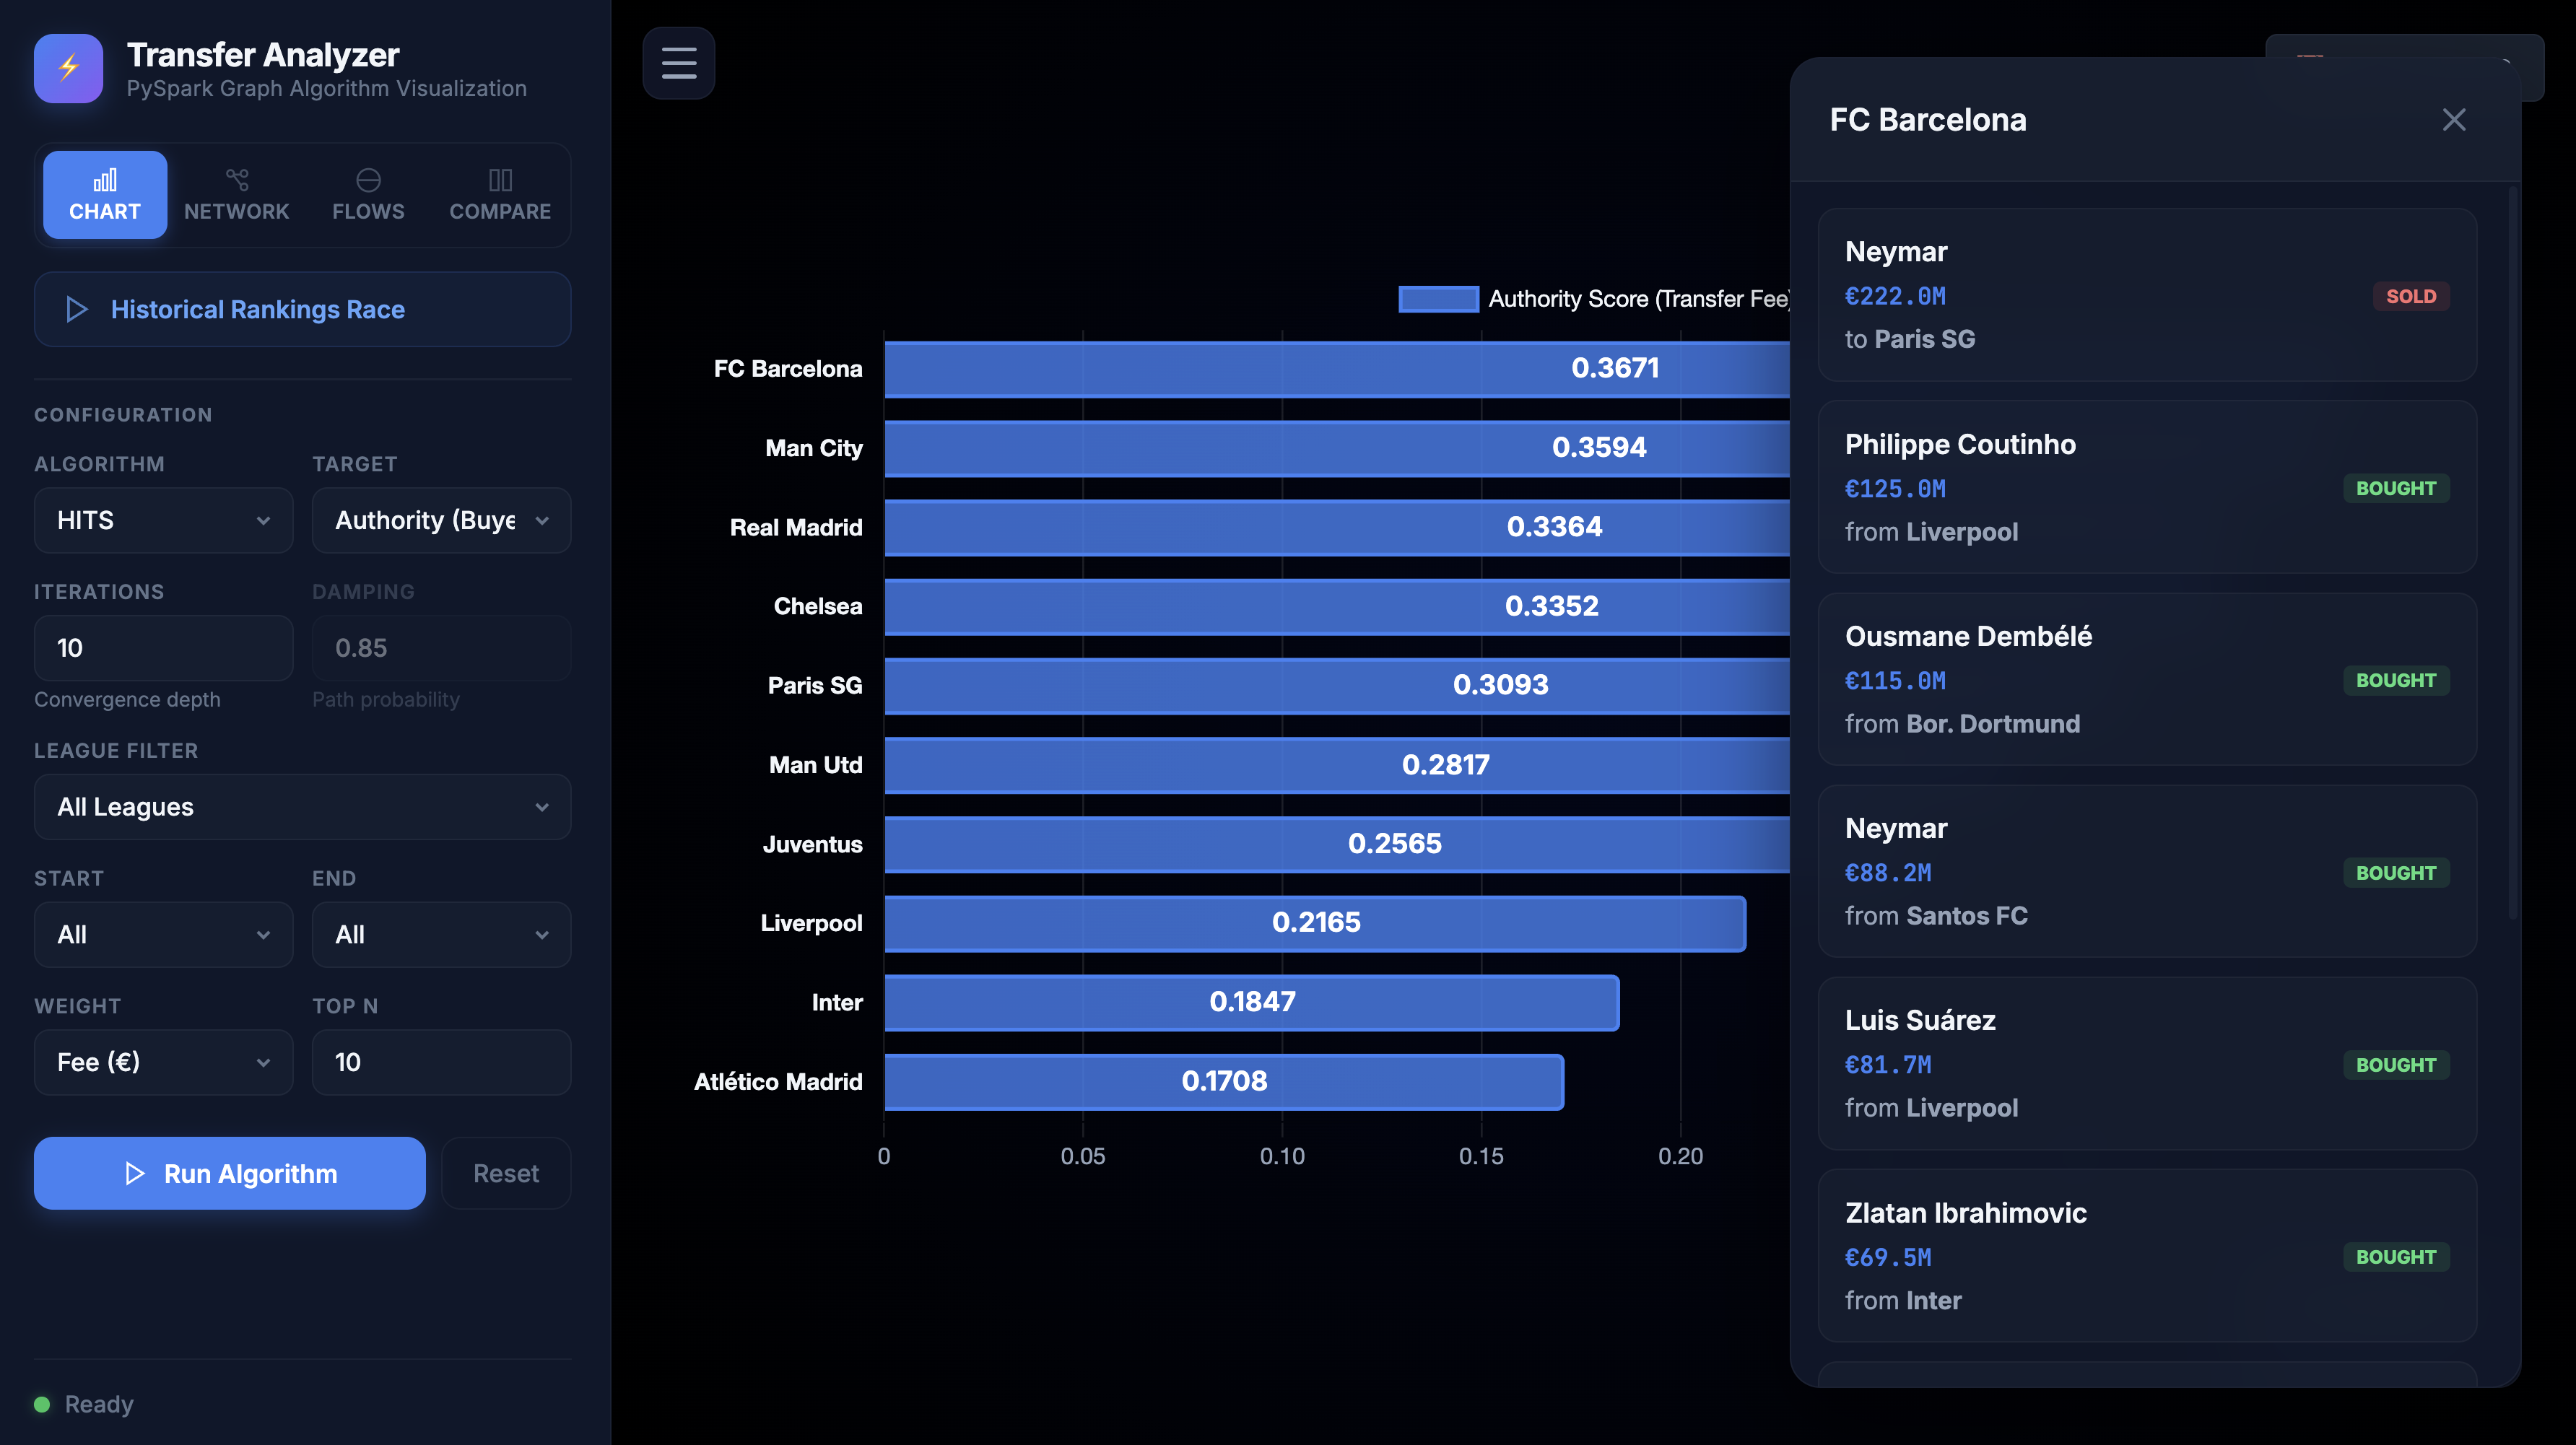
\includegraphics[width=1.0\textwidth]{Figures/ui_transfer_details.png}
    \caption{Transfer Details Panel displaying individual transfer records for a selected club.}
    \label{fig:ui_transfer_details}
\end{figure}

\subsection{Case Study: FC Barcelona Across the Years}
\label{subsec:results_barcelona_case}

To move beyond aggregate comparison and demonstrate the practical value of the developed system, this thesis also considers a concrete club-level case study. FC Barcelona is an appropriate example because it is one of the most visible clubs in the dataset and because its role in the transfer market changes substantially across years, making it well suited for longitudinal analysis.

Using the historical ranking logic of the implemented system, FC Barcelona was tracked season by season under the same algorithmic settings. The resulting pattern shows that the club is not uniformly dominant across the whole timeline; rather, its prominence rises strongly in some periods and declines sharply in others depending on the algorithm and weighting mode.

Under \textbf{fee-weighted PageRank}, FC Barcelona appeared in the top 10 in 6 out of the 19 analyzed seasons and entered the top 5 in 3 seasons. Its strongest period occurred in the late 2000s and mid-2010s. In particular, FC Barcelona ranked \textbf{2nd} in the 2008-2009 and 2009-2010 seasons.

\begin{figure}[htbp]
    \centering
    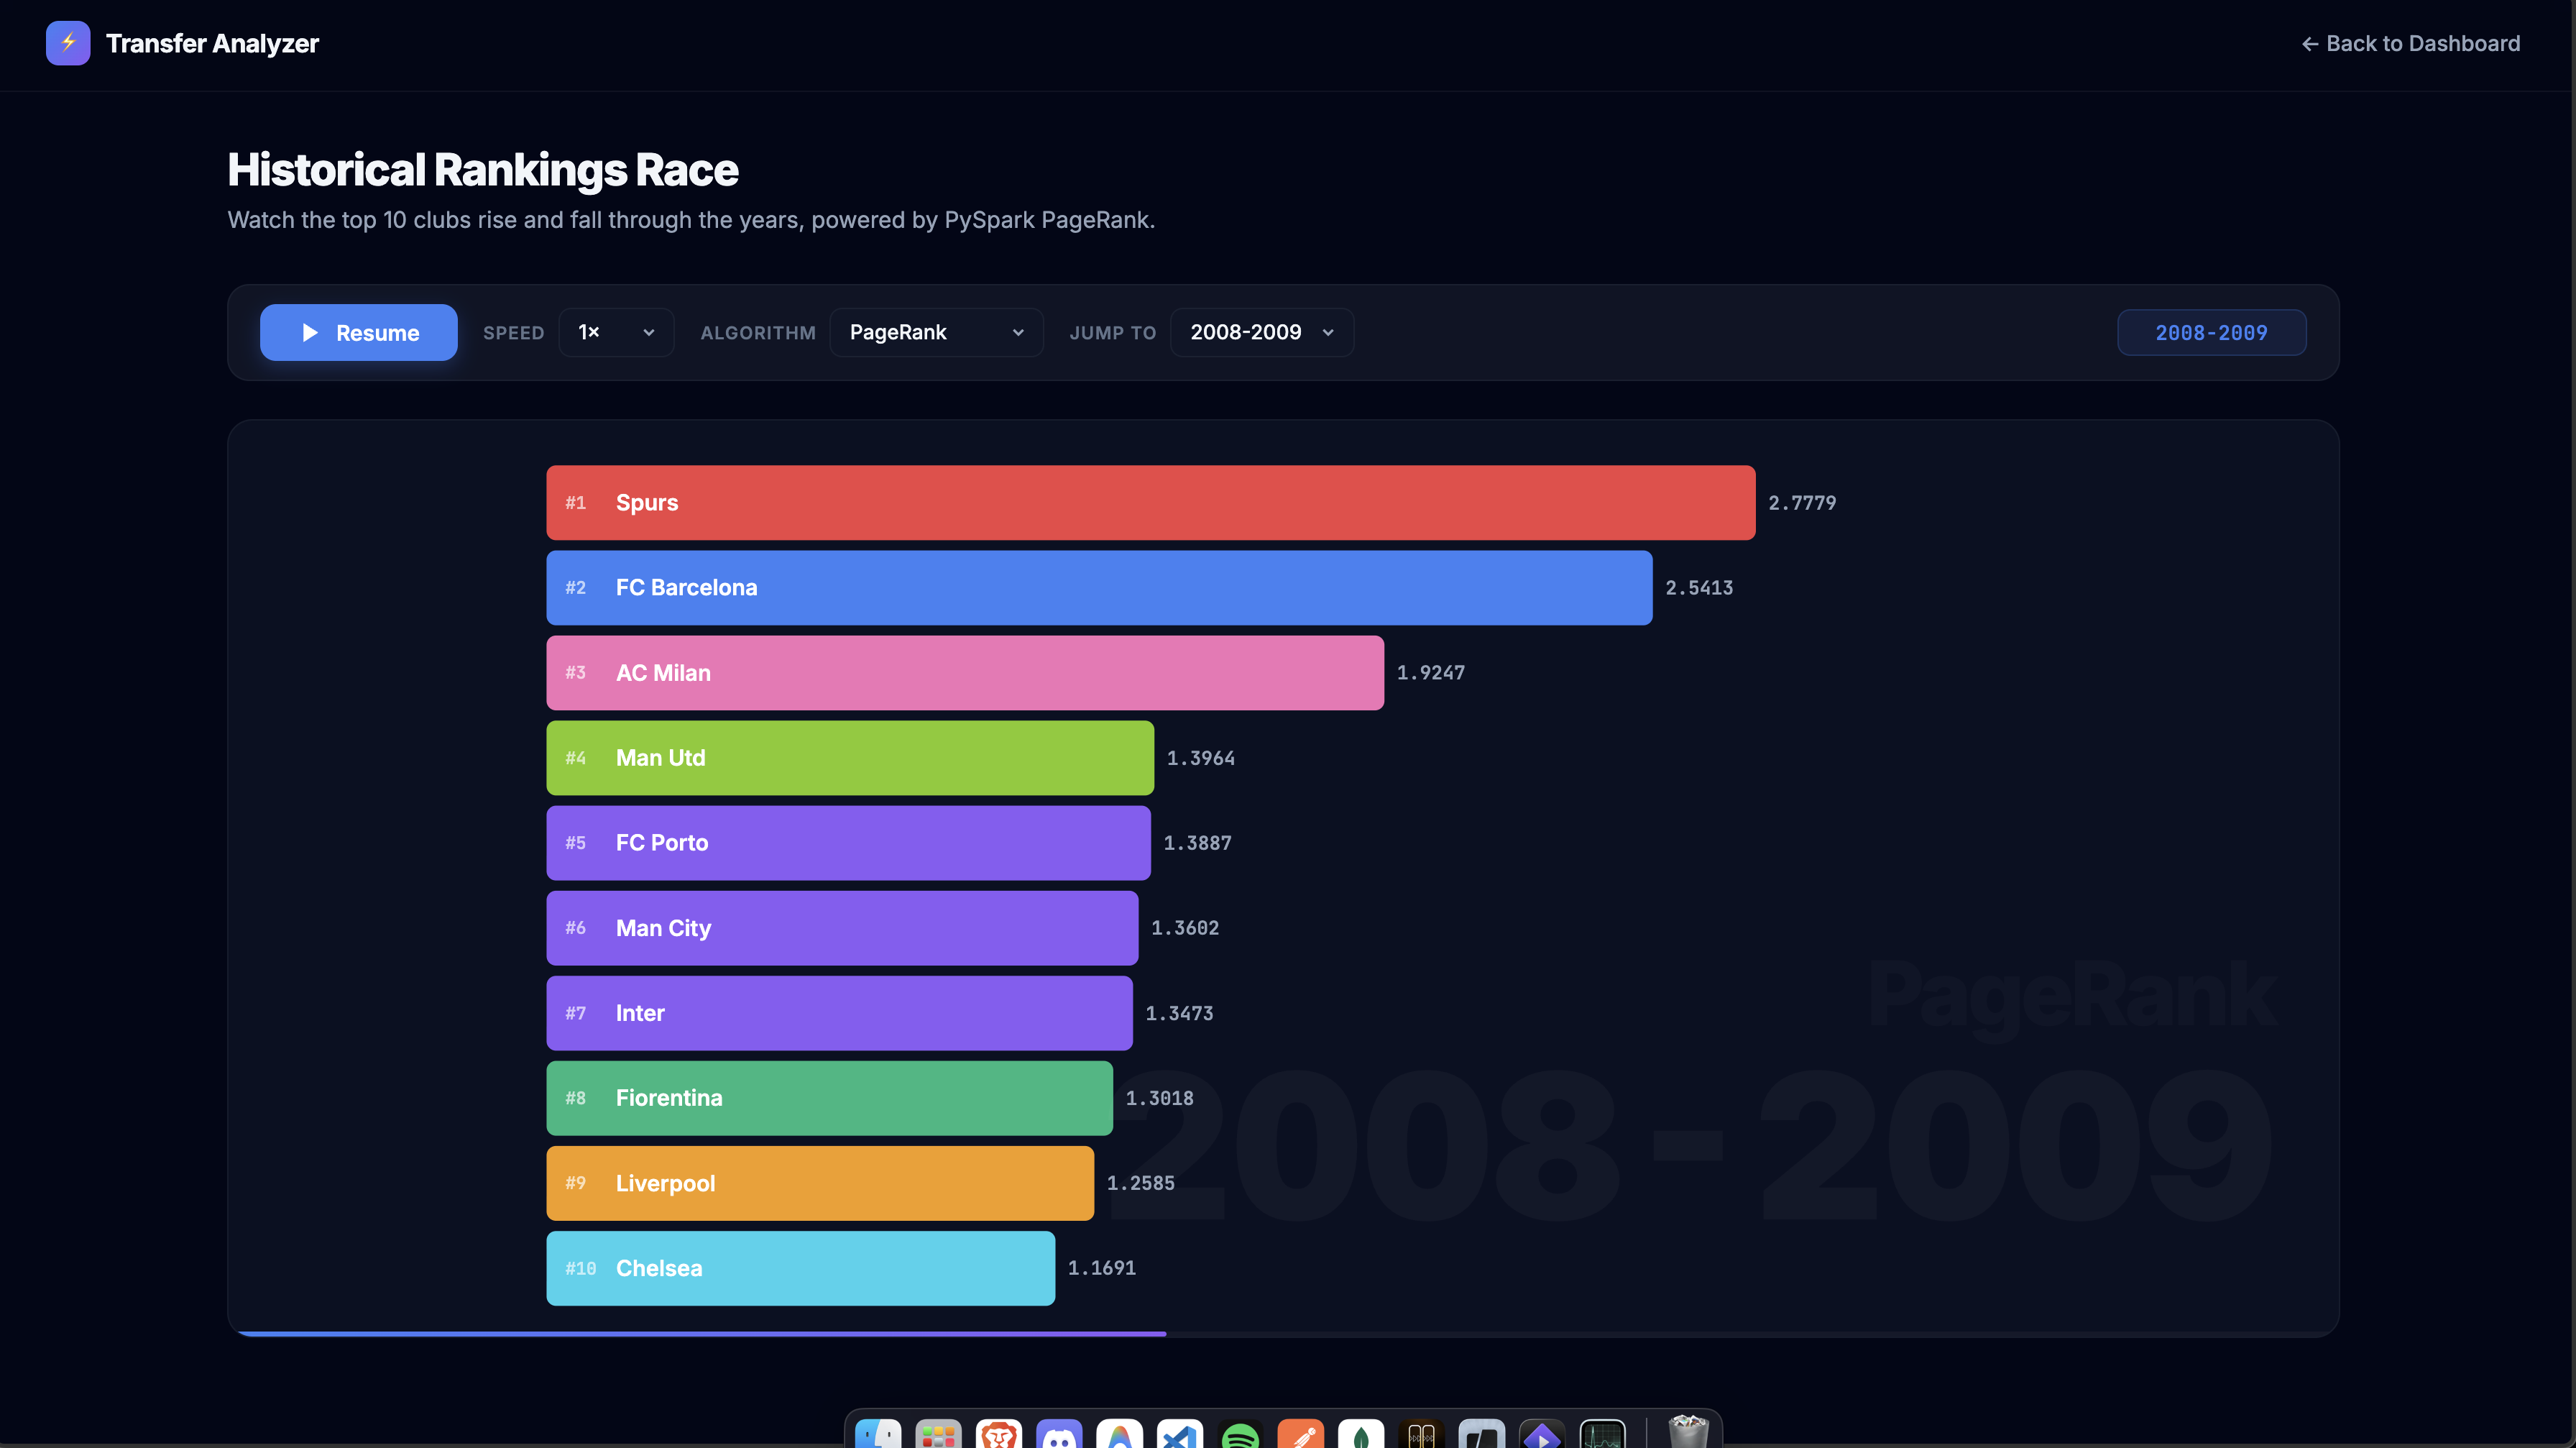
\includegraphics[width=1.0\textwidth]{Figures/barcelona_2009.png}
    \caption{FC Barcelona's strong position in the 2008-2009 season.}
    \label{fig:barcelona_2009}
\end{figure}

It then reached the absolute peak of its centrality by claiming \textbf{1st place} in the 2014-2015 season. 

\begin{figure}[htbp]
    \centering
    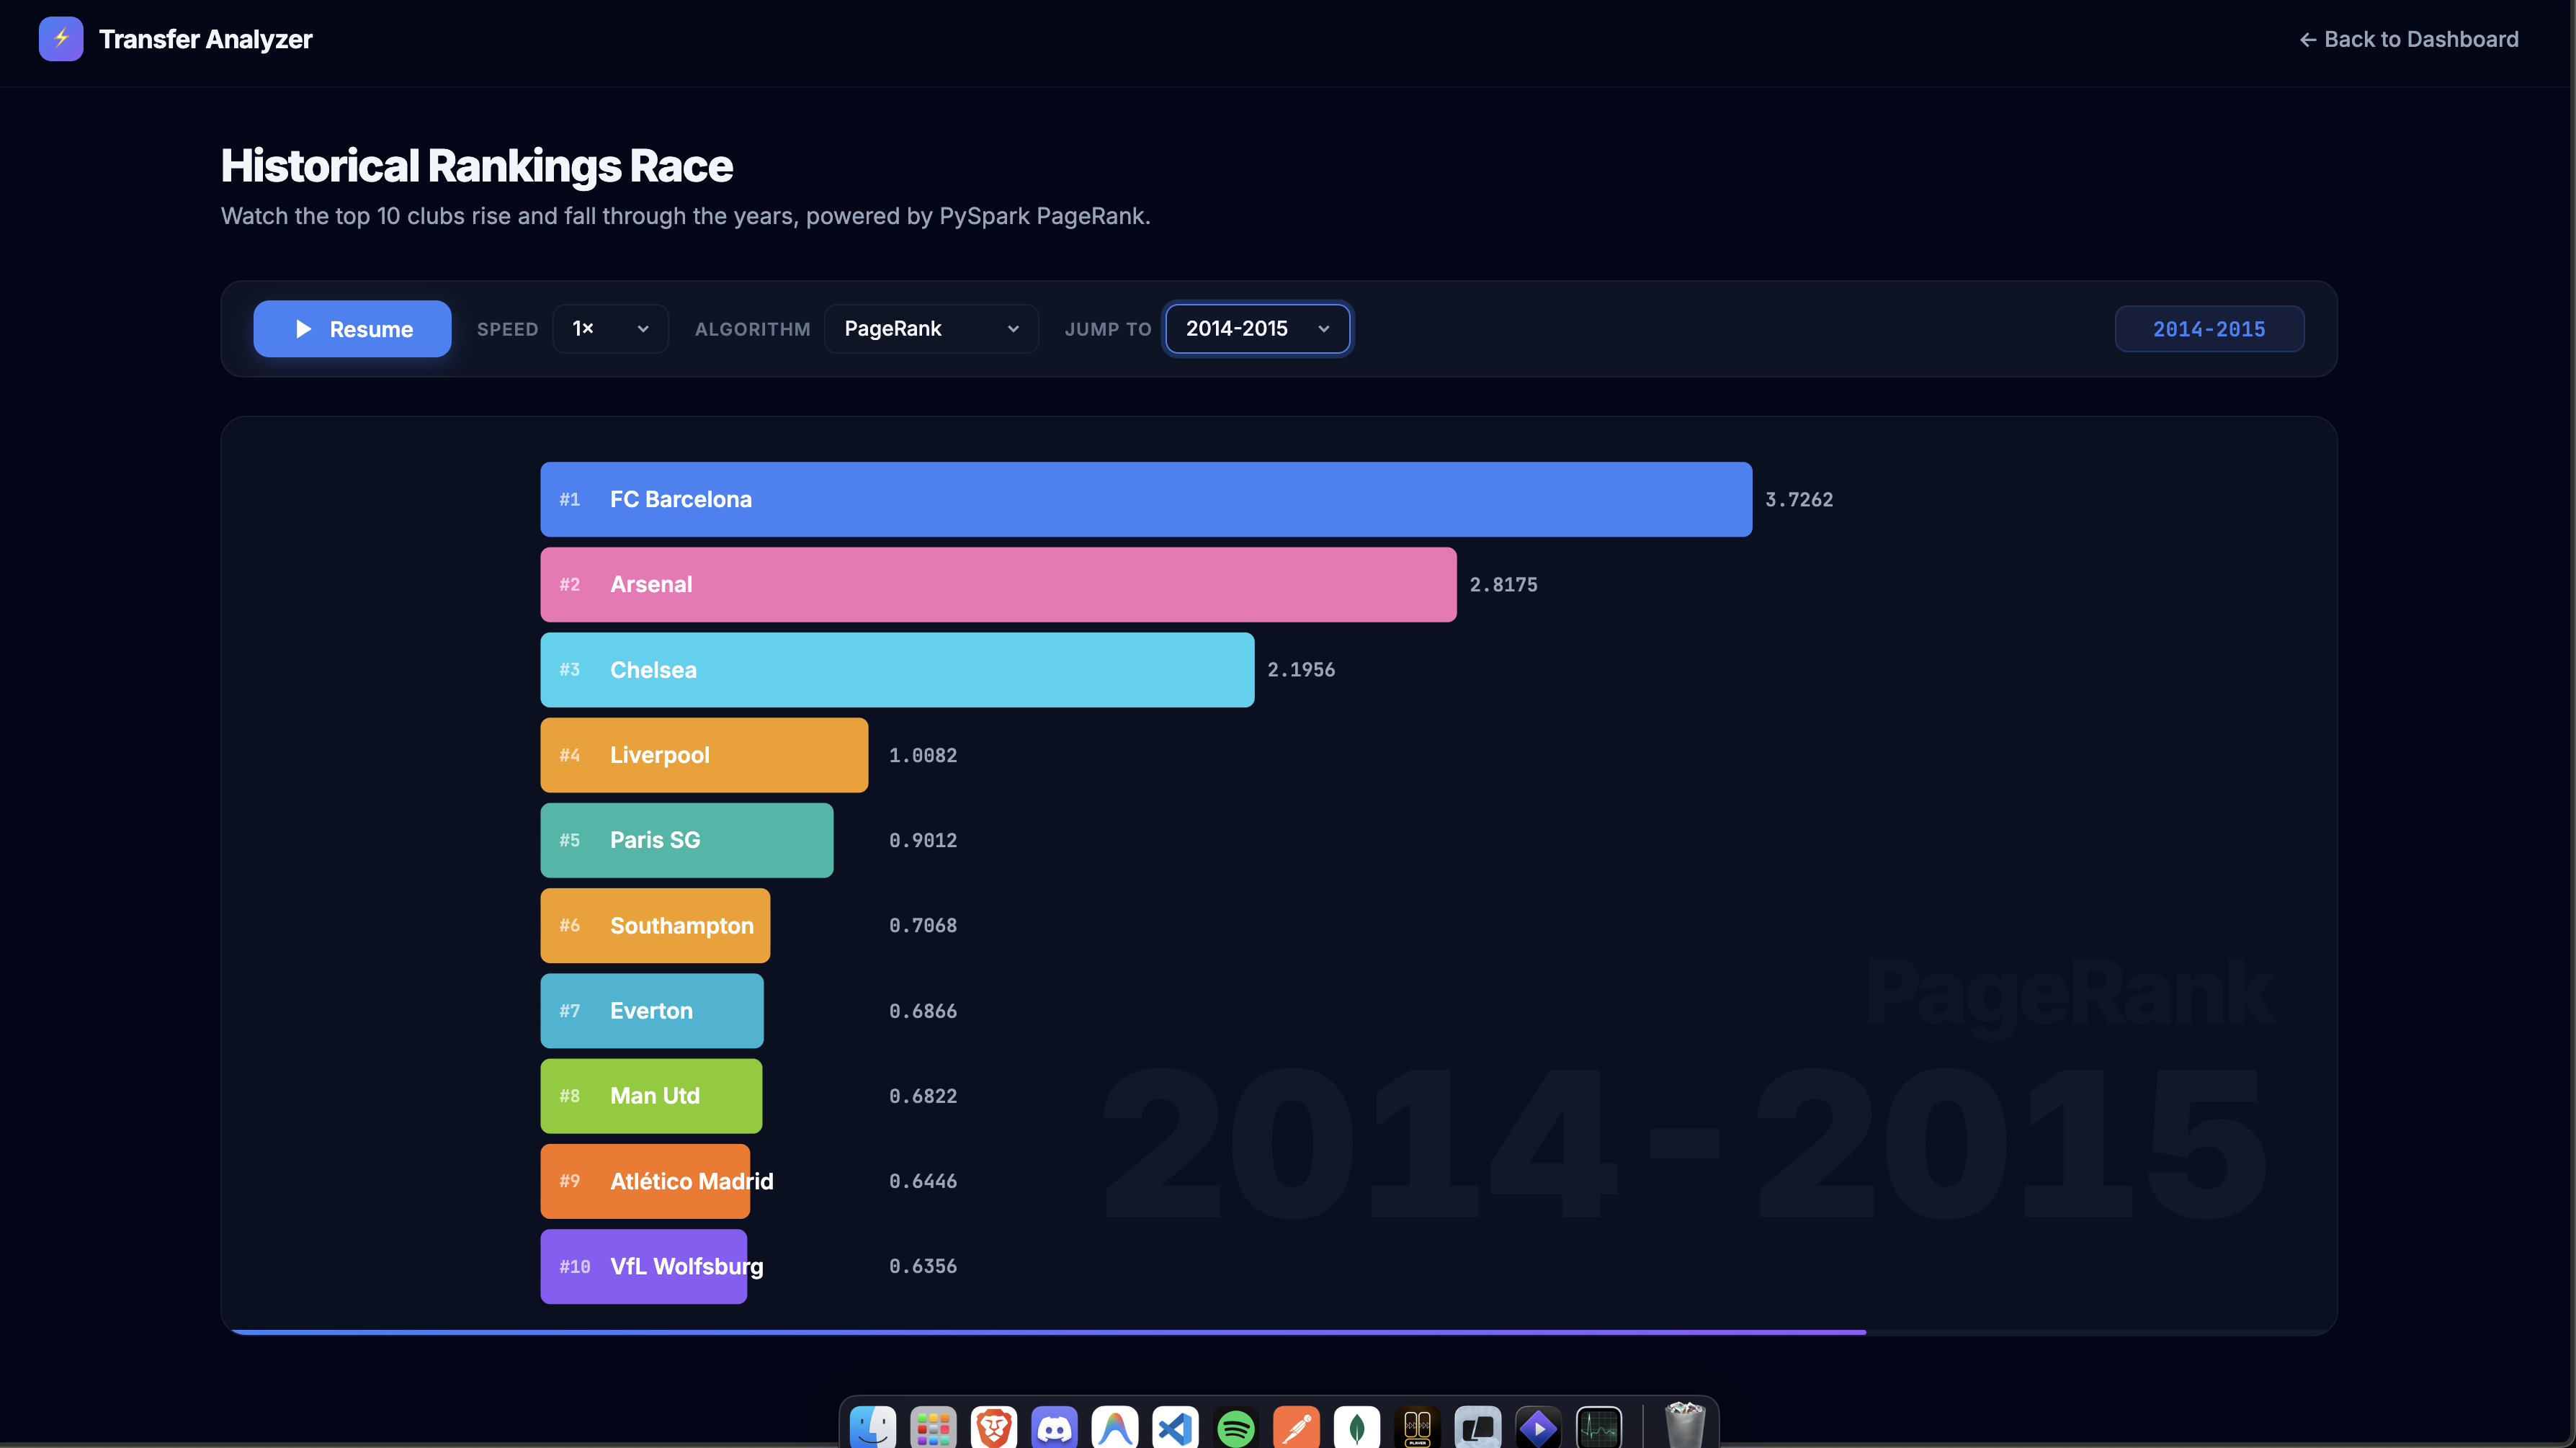
\includegraphics[width=1.0\textwidth]{Figures/barcelona_2014.png}
    \caption{FC Barcelona reaching 1st place in PageRank during the 2014-2015 season.}
    \label{fig:barcelona_2014}
\end{figure}

By contrast, it fell far outside the top ranks in several other seasons, including 2002-2003, 2013-2014, 2015-2016, and 2018-2019. This behavior indicates that FC Barcelona's global transfer-market centrality was highly concentrated in certain high-impact periods rather than being uniformly dominant throughout the entire dataset.

\begin{figure}[htbp]
    \centering
    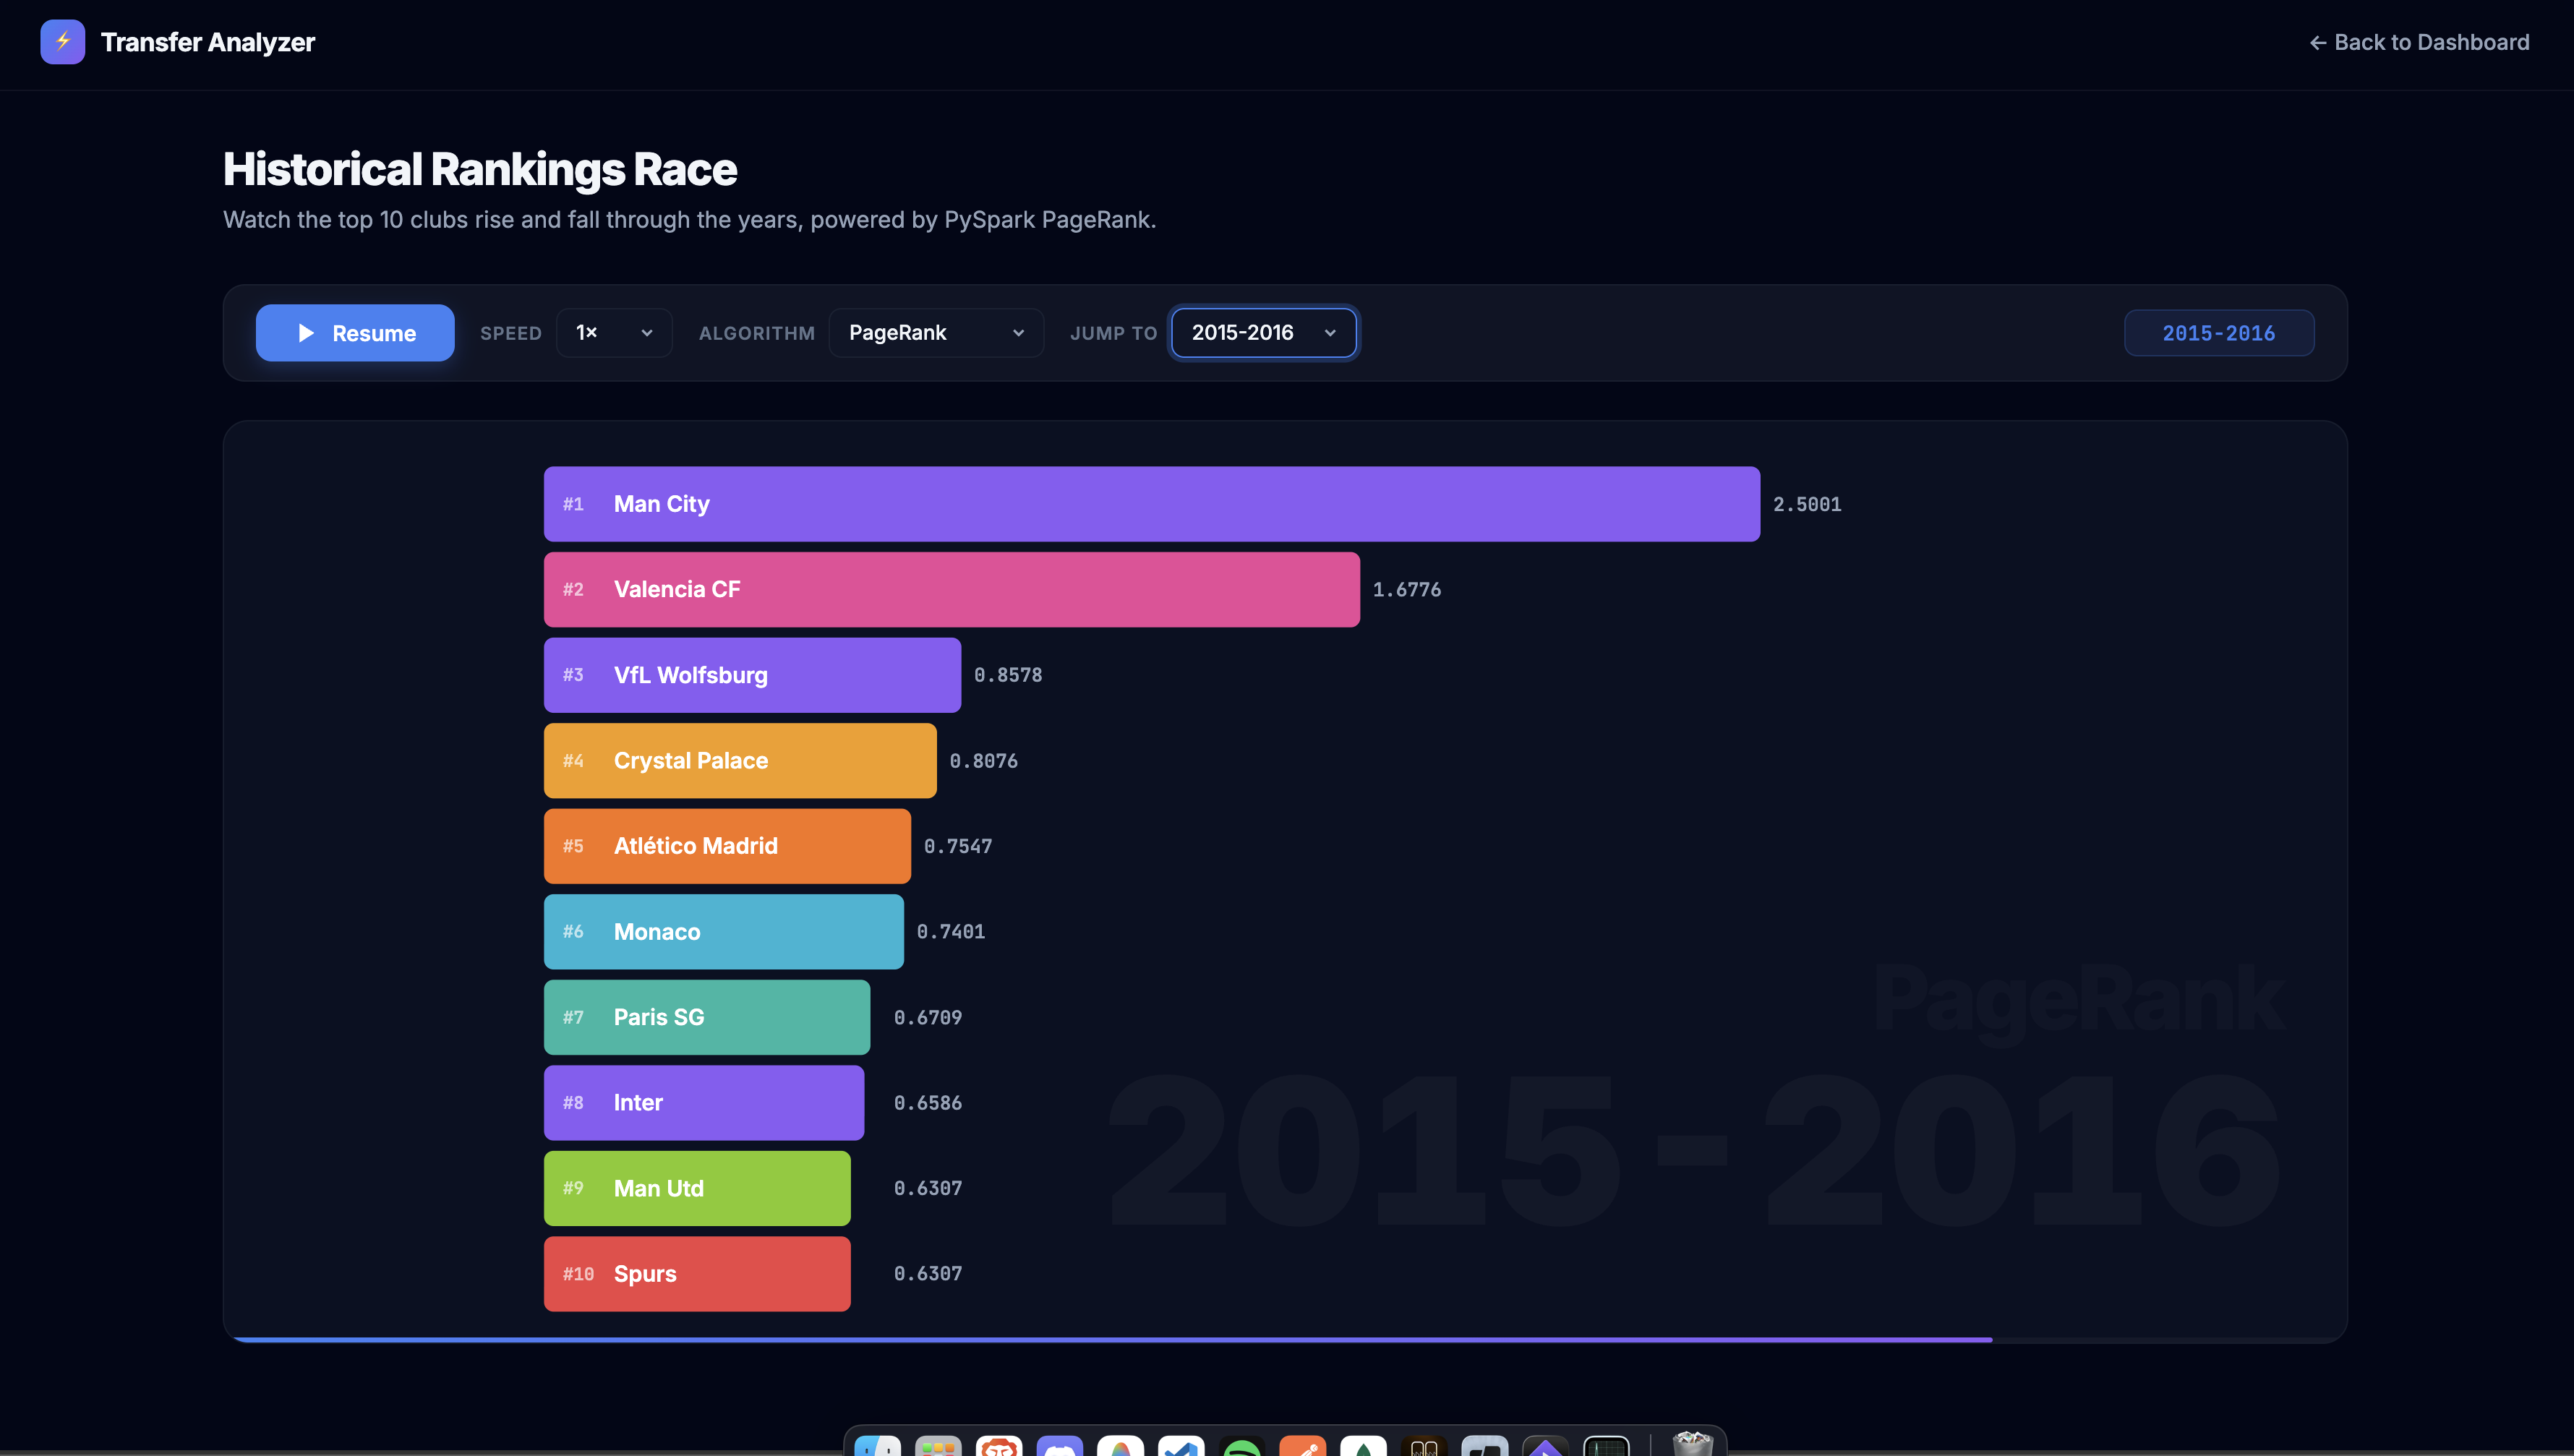
\includegraphics[width=1.0\textwidth]{Figures/barcelona_2015.png}
    \caption{FC Barcelona's ranking behavior in the 2015-2016 season.}
    \label{fig:barcelona_2015}
\end{figure}

Under \textbf{fee-weighted HITS authority}, the picture is different. FC Barcelona appeared in the top 10 in 9 seasons and in the top 5 in 7 seasons, which is more stable than its PageRank top-5 presence. It ranked \textbf{2nd} in 2000-2001, 2004-2005, 2010-2011, 2011-2012, and 2017-2018, and remained highly visible as an authority club in several other years even when its PageRank position was lower. This suggests that FC Barcelona repeatedly functioned as a structurally important \emph{destination} club, receiving players from well-connected supplier clubs, even in seasons where it was not globally dominant in PageRank terms.

\begin{figure}[htbp]
    \centering
    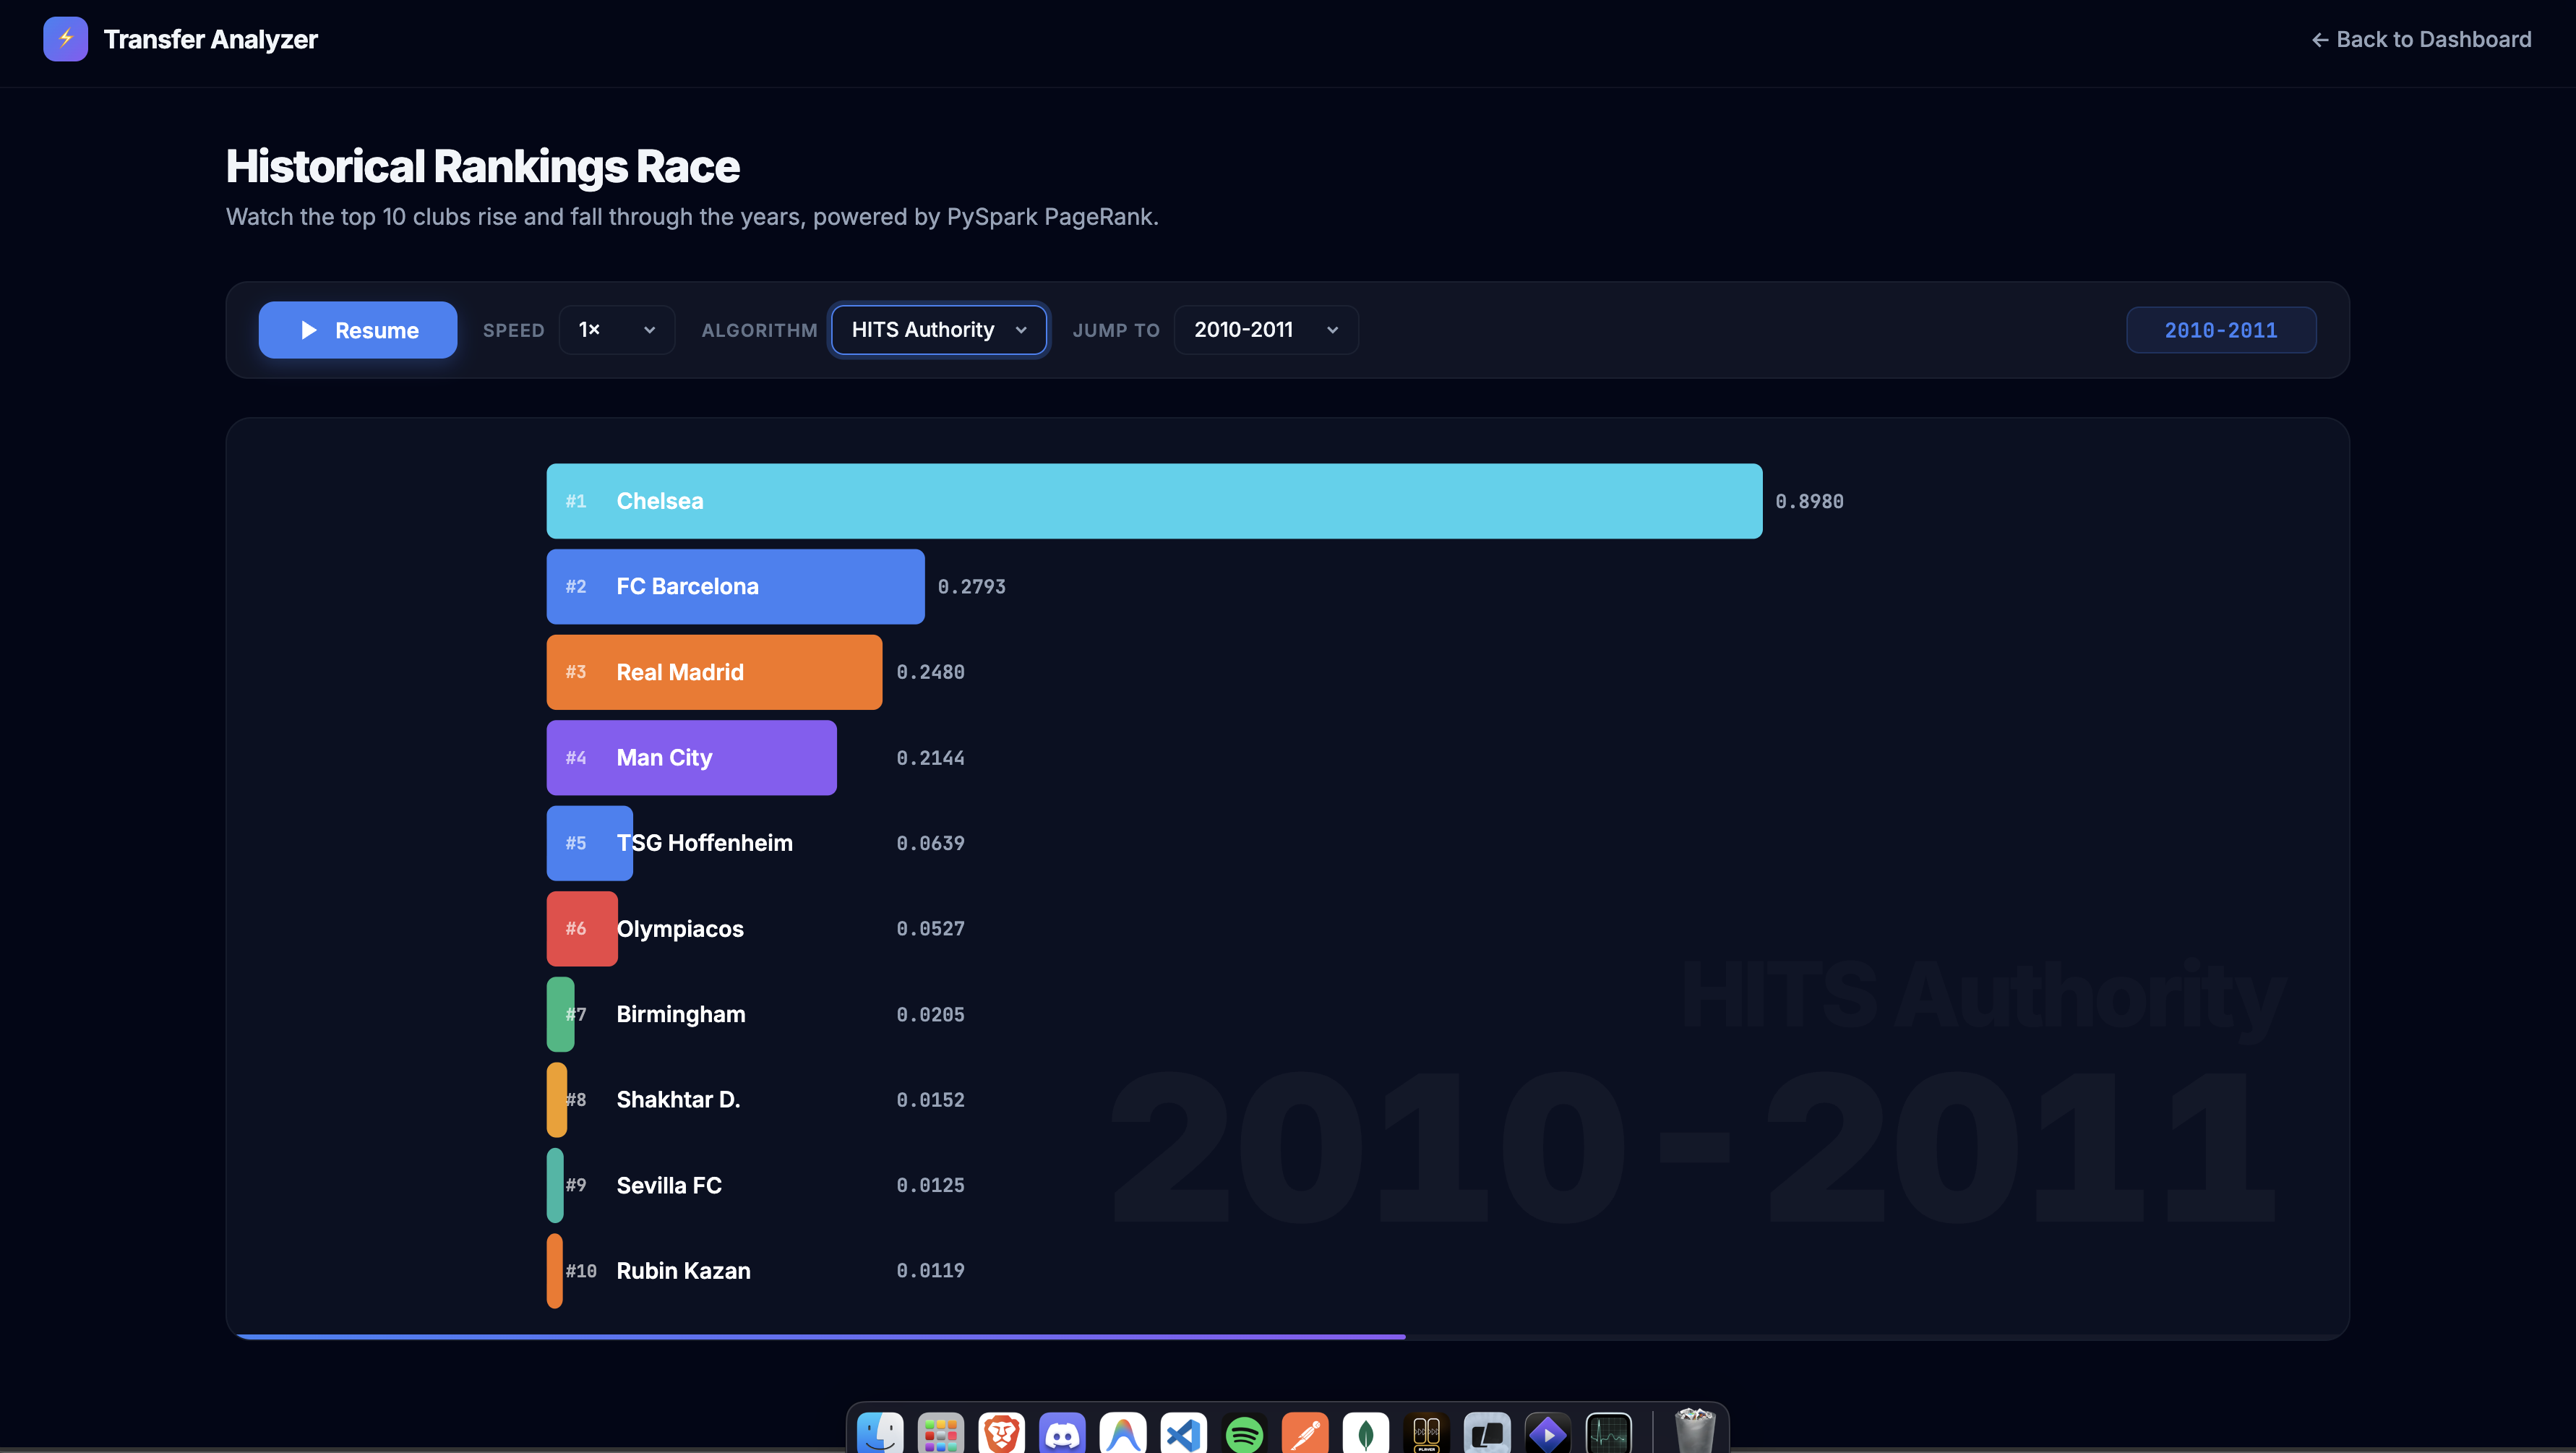
\includegraphics[width=1.0\textwidth]{Figures/barcelona_2010.png}
    \caption{FC Barcelona's ranking in the 2010-2011 season.}
    \label{fig:barcelona_2010}
\end{figure}

The contrast becomes even clearer when count-based weighting is considered. Under \textbf{count-weighted PageRank}, FC Barcelona reached the top 10 in only 4 seasons and the top 5 in only 2 seasons, with its best result again being \textbf{1st} in 2014-2015. Under \textbf{count-weighted HITS authority}, however, it still appeared in the top 10 in 8 seasons, including \textbf{2nd} place in 2000-2001 and 2009-2010, and strong positions in 2004-2005 and 2006-2007. This indicates that FC Barcelona's structural role is more consistently captured by authority-based analysis than by transaction-frequency-based global centrality.

Taken together, these results support an important substantive conclusion. FC Barcelona's importance in the transfer network is not explained simply by the number of transfers it performs. Instead, its prominence is more strongly associated with the \emph{quality and structural importance} of the clubs from which it acquires players and, in its strongest years, with its participation in financially significant transfer exchanges. In other words, FC Barcelona is better characterized as a repeatedly strong \textbf{authority} club and a periodically dominant \textbf{PageRank} club, rather than as a consistently high-volume transfer actor.

\begin{table}[H]
\centering
\resizebox{\textwidth}{!}{%
\begin{tabular}{|l|c|c|c|c|}
\hline
\textbf{Algorithm \& Weight} & \textbf{Total Top-10} & \textbf{Total Top-5} & \textbf{Best Rank} & \textbf{Best Year(s)} \\
\hline
PageRank (Fee) & 6 & 3 & 1st & 2014-2015 \\
HITS Authority (Fee) & 9 & 7 & 2nd & 2000-01, 2004-05, 2010-11, 2011-12, 2017-18 \\
PageRank (Count) & 4 & 2 & 1st & 2014-2015 \\
HITS Authority (Count) & 8 & 4 & 2nd & 2000-01, 2009-10 \\
\hline
\end{tabular}%
}
\caption{Summary of FC Barcelona's Rankings Across Seasons (Out of 19 Total Seasons)}
\label{tab:barcelona_case_study}
\end{table}

This case study illustrates the broader value of the thesis approach. If only one algorithm had been used, the interpretation of FC Barcelona's historical role would have been incomplete. PageRank highlights the years in which the club occupied a globally central position in the weighted transfer ecosystem, whereas HITS authority highlights the years in which it acted as a major destination for talent from structurally important suppliers. The season-by-season analysis therefore reinforces the thesis's central argument that transfer-market importance is dynamic, multi-dimensional, and dependent on the ranking method used.


%=============================================================
\section{Comparative Discussion of Findings}
\label{sec:results_discussion}

The most important result of the thesis is that PageRank and HITS do not simply provide duplicate rankings under different names. Instead, they illuminate different structural aspects of the same transfer network.

PageRank is more naturally interpreted as a measure of global transfer-market centrality. It identifies clubs that occupy influential positions in the overall directed flow of player movement. HITS, by contrast, provides a two-role decomposition that distinguishes destination power from supplier power. This distinction is particularly useful in football transfer analysis because the market contains clubs that mainly attract talent, clubs that mainly supply talent, and clubs that participate in both roles.

The weighting comparison further strengthens this conclusion. Fee-based analysis emphasizes economic influence, while count-based analysis emphasizes interaction frequency. League and season filters then show that these notions of influence are context dependent rather than universal. Together, these findings support the central claim of the thesis: the value of comparing PageRank and HITS lies not in choosing a single winner, but in understanding how each algorithm highlights a different dimension of network structure.


%=============================================================
\section{Chapter Summary}
\label{sec:results_summary}

This chapter presented the results framework for interpreting PageRank and HITS on the football transfer network. The analysis considered buyer and seller perspectives, fee-based and count-based weighting, league and season filtering, and multiple visualization modes including ranked charts, network graphs, league flows, compare mode, and historical animation.

Taken together, the results show that the football transfer market is not adequately described by a single notion of importance. Instead, different algorithmic and visual perspectives reveal different forms of influence, centrality, supply behavior, and temporal evolution. The next chapter concludes the thesis by summarizing the main contributions and outlining directions for future work.
